\documentclass{article}
\usepackage{enumerate}
\usepackage{enumitem}
\usepackage[utf8]{inputenc}
\usepackage{latexsym,amsfonts,amssymb,amsthm,amsmath}
\usepackage{graphicx}
\usepackage{caption}
\usepackage{subfigure}
\usepackage{float}
\usepackage{bbm}
\usepackage{tcolorbox}
\usepackage{indentfirst}
\usepackage[a4paper, margin=0.5in]{geometry}
\newcommand{\norm}[1]{\left\lVert#1\right\rVert}
\usepackage[colorlinks=true]{hyperref}
\pagenumbering{gobble}
\newcommand*{\re}{\mathbb{R}}
\newcommand*{\normal}{\mathcal{N}}

\title{COL778: Principles of Autonomous Systems\\Assignment 2}
\author{Harshit Goyal (2021MT10143)}
\date{March 2025}
\begin{document}
\maketitle
Please find the project repository \href{https://github.com/Harshit0143/COL778-Principles-of-Autonomous-System/tree/main/Assignment2}{here}.\\
\tableofcontents



\section{Tabular Q-Learning}
\subsection{Learning Policy}
\begin{figure}[H]
    \centering
    \begin{minipage}{0.49\linewidth}
        \centering
        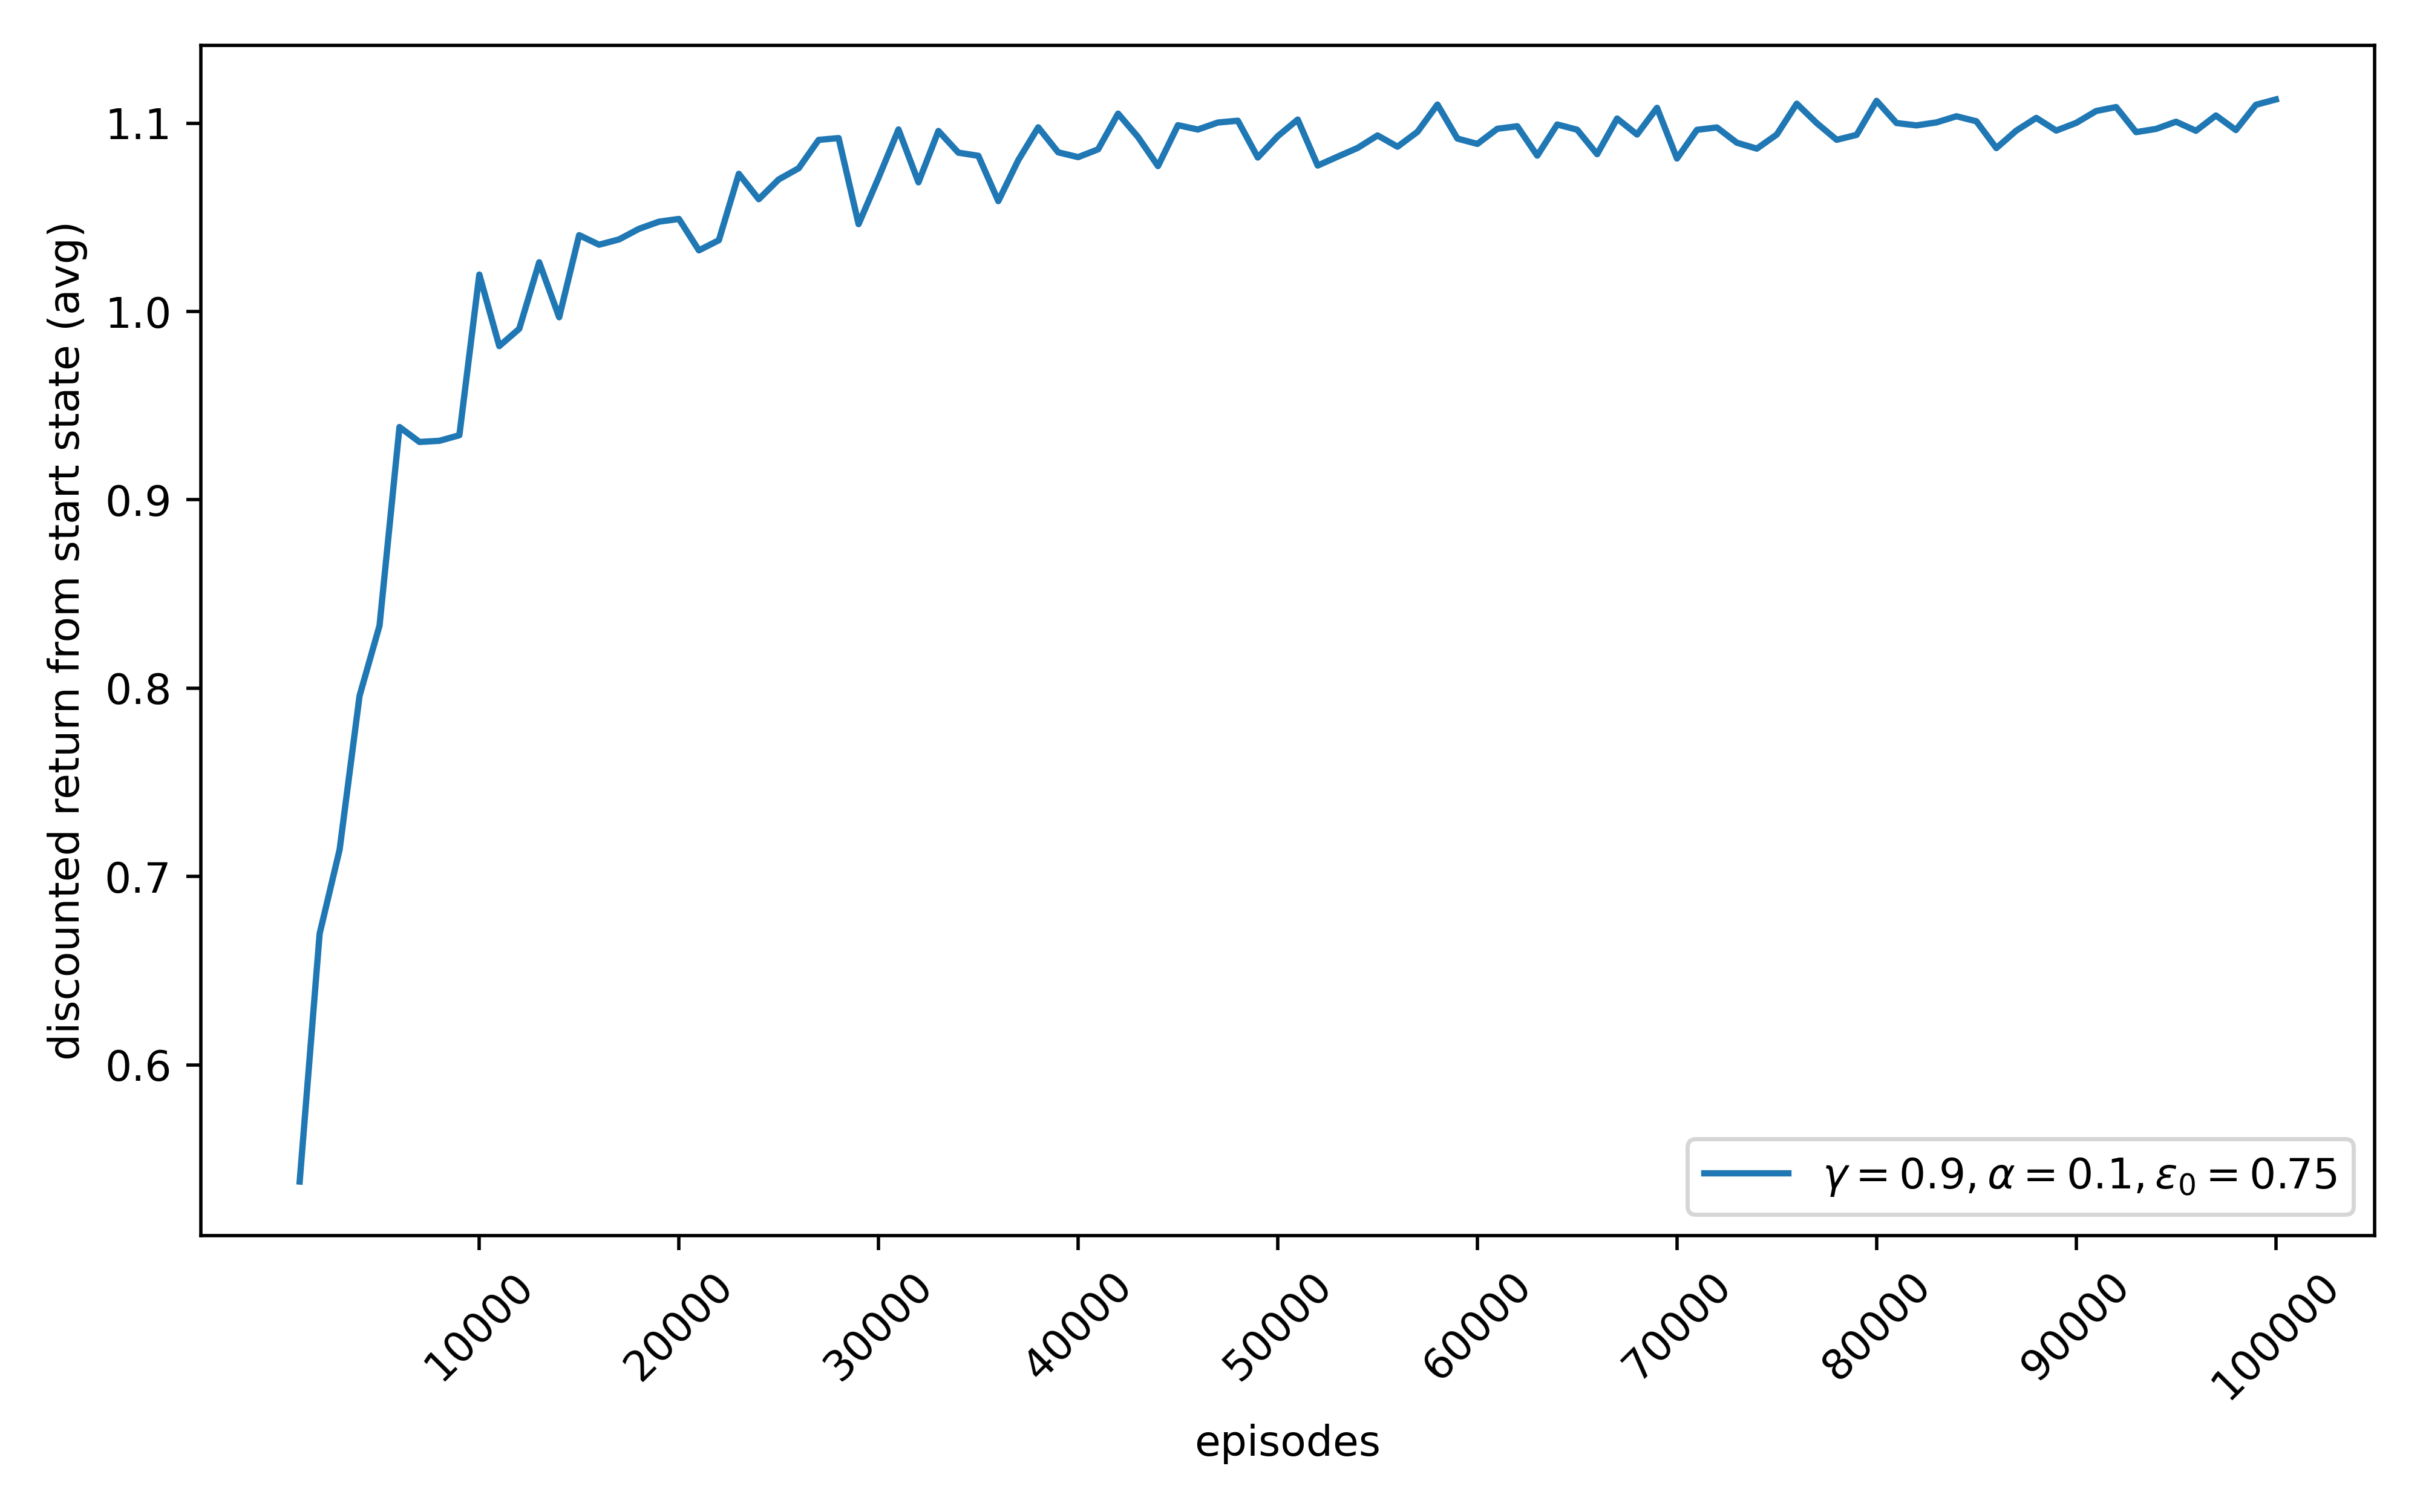
\includegraphics[width=\linewidth]{plots/part1-a-rewards.png}
        \caption{Discounted Return}
        
    \end{minipage}
    \hfill
    \begin{minipage}{0.49\linewidth}
        \centering
        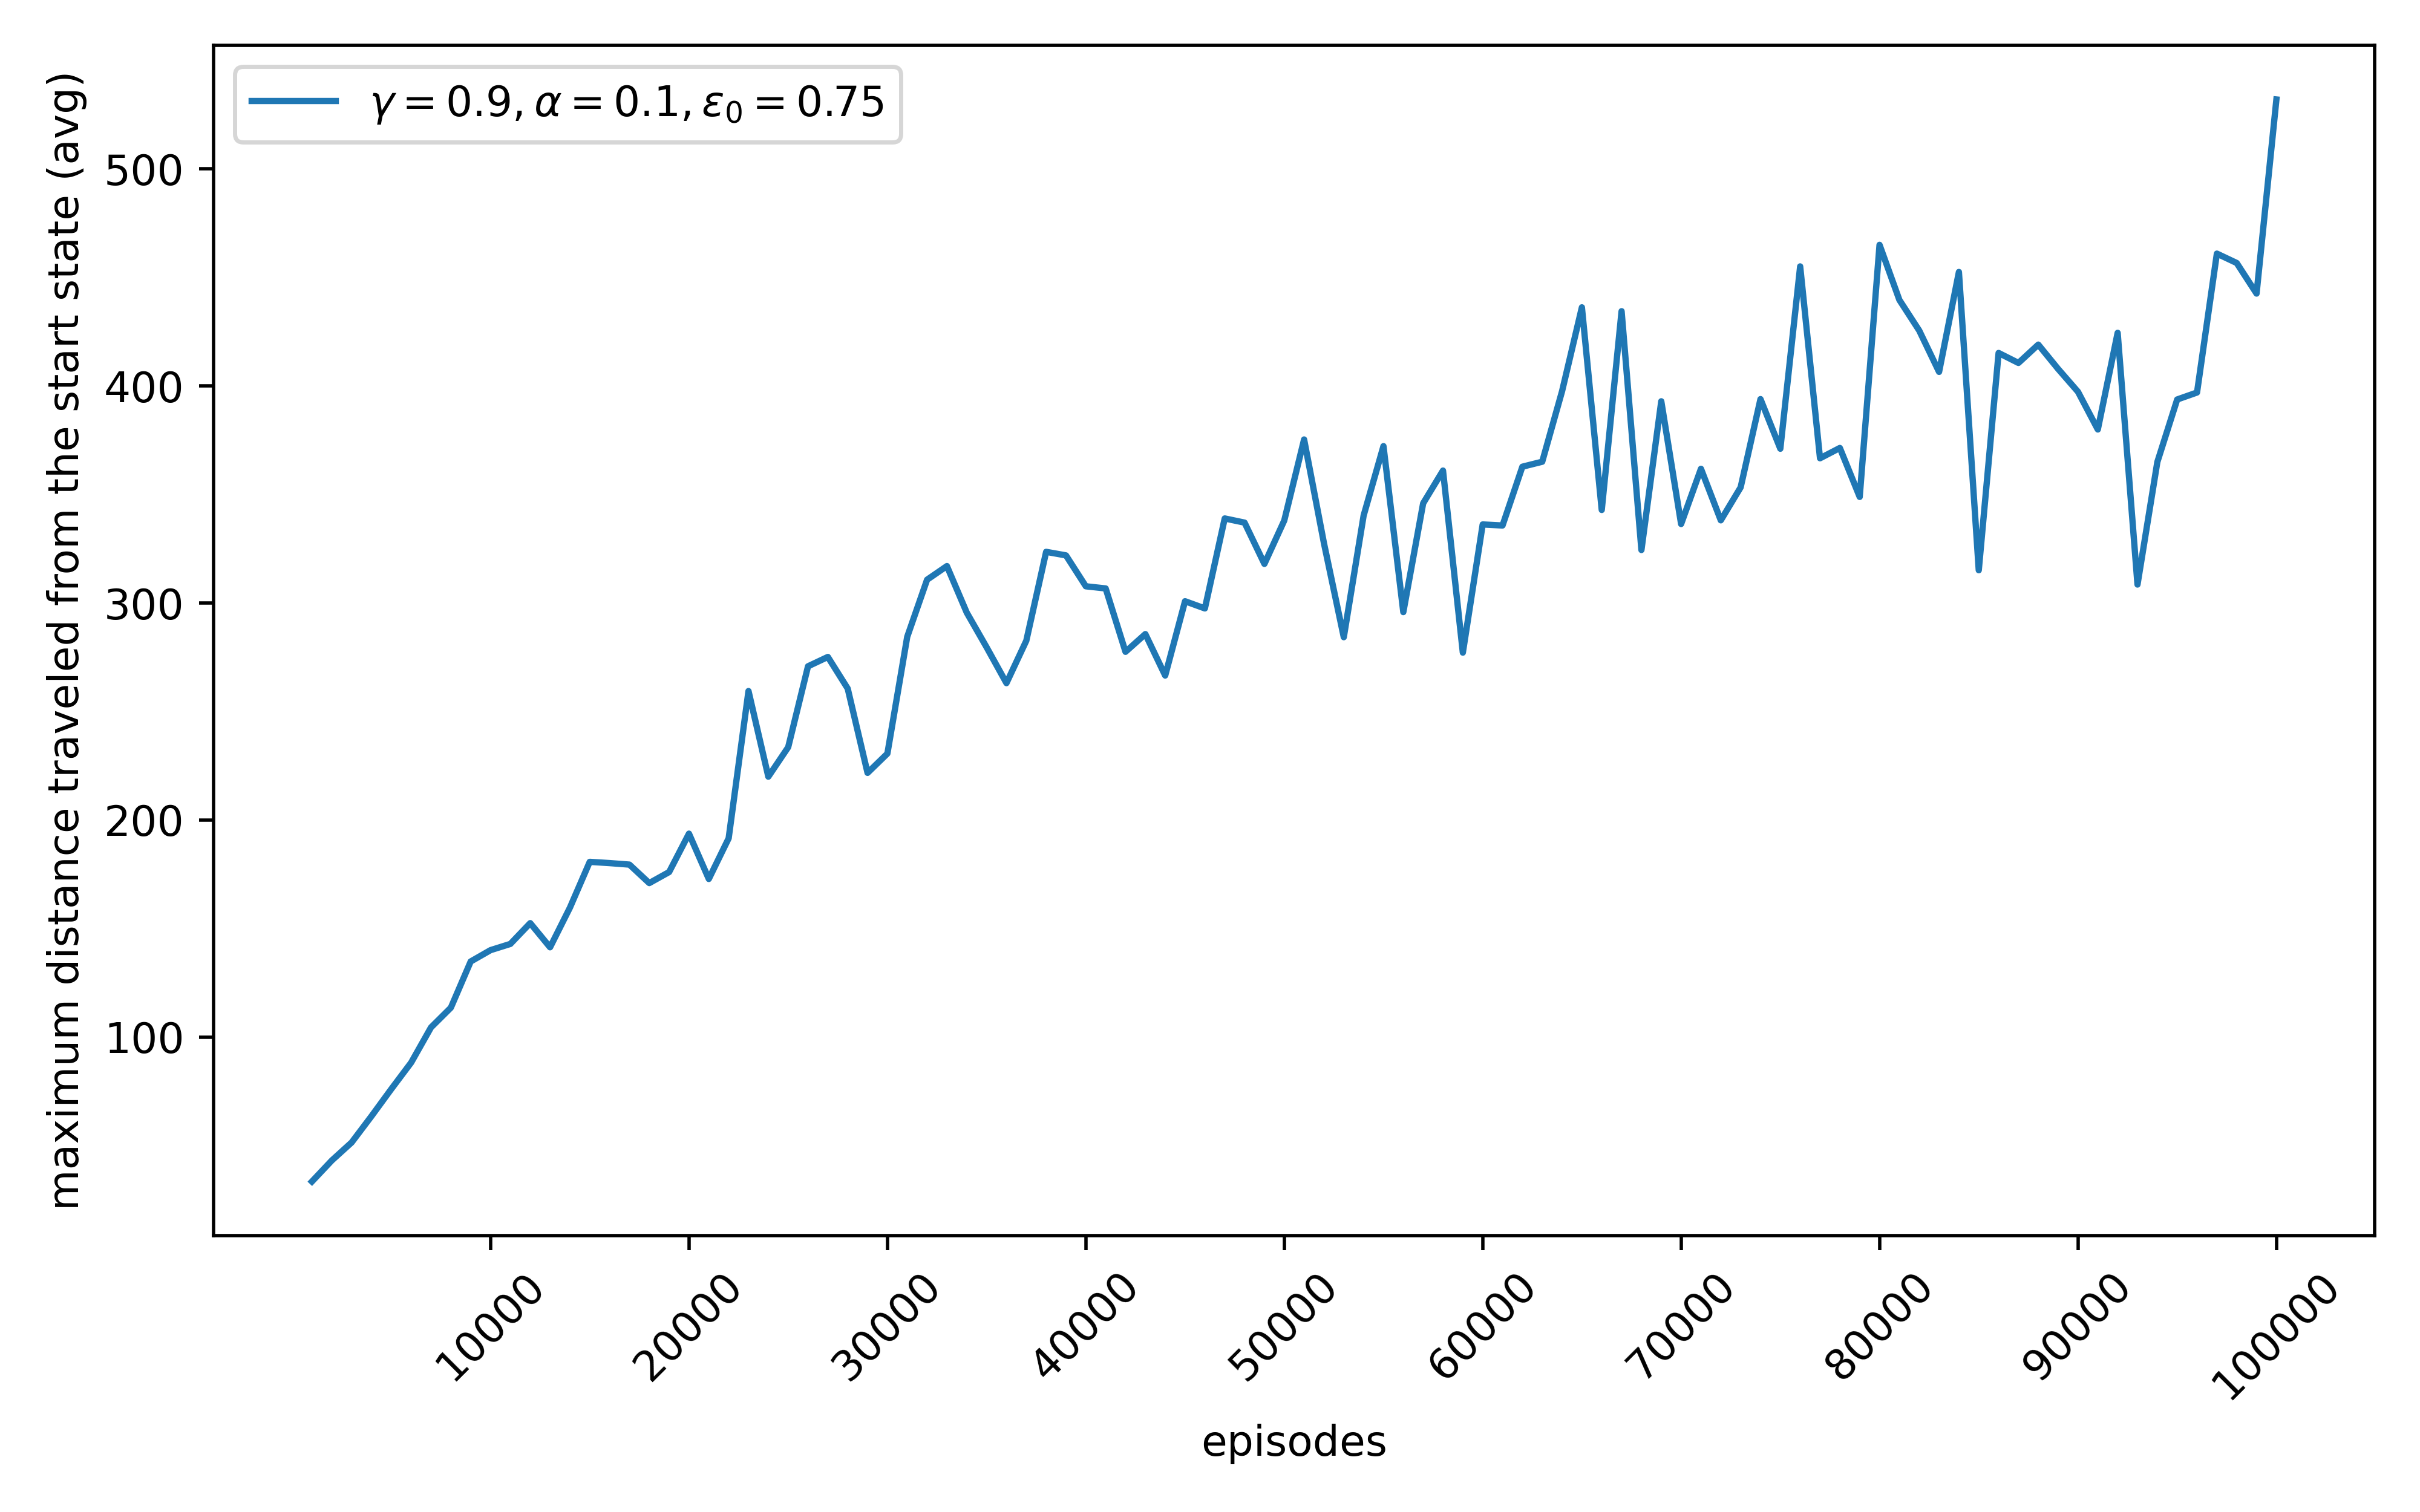
\includegraphics[width=\linewidth]{plots/part1-a-distances.png}
        \caption{Distance Traveled}
    \end{minipage}

    \vspace{1em}
    \begin{minipage}{\linewidth}
        \centering
        \begin{tabular}{lccc}
            \hline
            Episodes & Discounted Return & Average Distance \\
            \hline
            $50,000$ & $1.09$ & $338.00$ \\
            $98,000$ & $1.10$ & $456.64$ \\
            $99,000$ & $1.11$ & $442.55$ \\
            $100,000$ & $1.11$ & $531.98$ \\
            \hline
        \end{tabular}
        \caption{\texttt{Tabular} $\gamma = 0.9, \alpha = 0.1, \epsilon = 0.75$}
    \end{minipage}
     \label{fig:part1-a}
\end{figure}
\subsection{Lane Visualization}

\begin{enumerate}
\item See \autoref{fig:part1-a-lane-visualization}. \texttt{Black} to \texttt{white} represents increasing Q-value. Note that colors in two different visualizations are not to the same scale.
\item The agent assigns highest value to the lane where it can avoid collision for the longest time.
\item The agent also seems to value a lane based on value if lane(s) adjacent to it. 
\end{enumerate}

\begin{figure}[H]
    \centering
    \begin{minipage}[t]{0.48\textwidth}
        \centering
        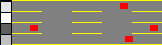
\includegraphics[width=\linewidth]{plots/part1-a-lane_visualization_00_step_0240.png}
    \end{minipage}
    \hfill
    \begin{minipage}[t]{0.48\textwidth}
        \centering
        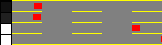
\includegraphics[width=\linewidth]{plots/part1-a-lane_visualization_00_step_0260.png}
    \end{minipage}
    
    \vspace{2mm}
    
    \begin{minipage}[t]{0.48\textwidth}
        \centering
        
\includegraphics[width=\linewidth]{plots/part1-a-lane_visualization_01_step_0340.png}
    \end{minipage}
    \hfill
    \begin{minipage}[t]{0.48\textwidth}
        \centering
        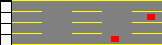
\includegraphics[width=\linewidth]{plots/part1-a-lane_visualization_01_step_0600.png}
    \end{minipage}
    \caption{Lane visualization for Tabular Q-agent}
    \label{fig:part1-a-lane-visualization}
\end{figure}

\subsection{Speed Visualization}
\begin{enumerate}
\item Note that \texttt{speed = 4} is always black due to the environment.
\item See \autoref{fig:part1-a-speed-visualization}. The agent prefers higher speed when the obstacle is farther away.
\end{enumerate}

\begin{figure}[H]
    \centering
    \begin{minipage}{0.48\textwidth}
        \centering
        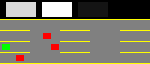
\includegraphics[width=\linewidth]{plots/part1-a-speed_visualization_00_step_0120.png}
    \end{minipage}
    \hfill
    \begin{minipage}{0.48\textwidth}
        \centering
        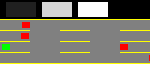
\includegraphics[width=\linewidth]{plots/part1-a-speed_visualization_00_step_0260.png}
    \end{minipage}
    \caption{Speed visualization for Tabular Q-agent}
    \label{fig:part1-a-speed-visualization}
\end{figure}





\subsection{Varying $\gamma$}
\begin{figure}[H]
    \centering
    \begin{minipage}{0.49\linewidth}
        \centering
        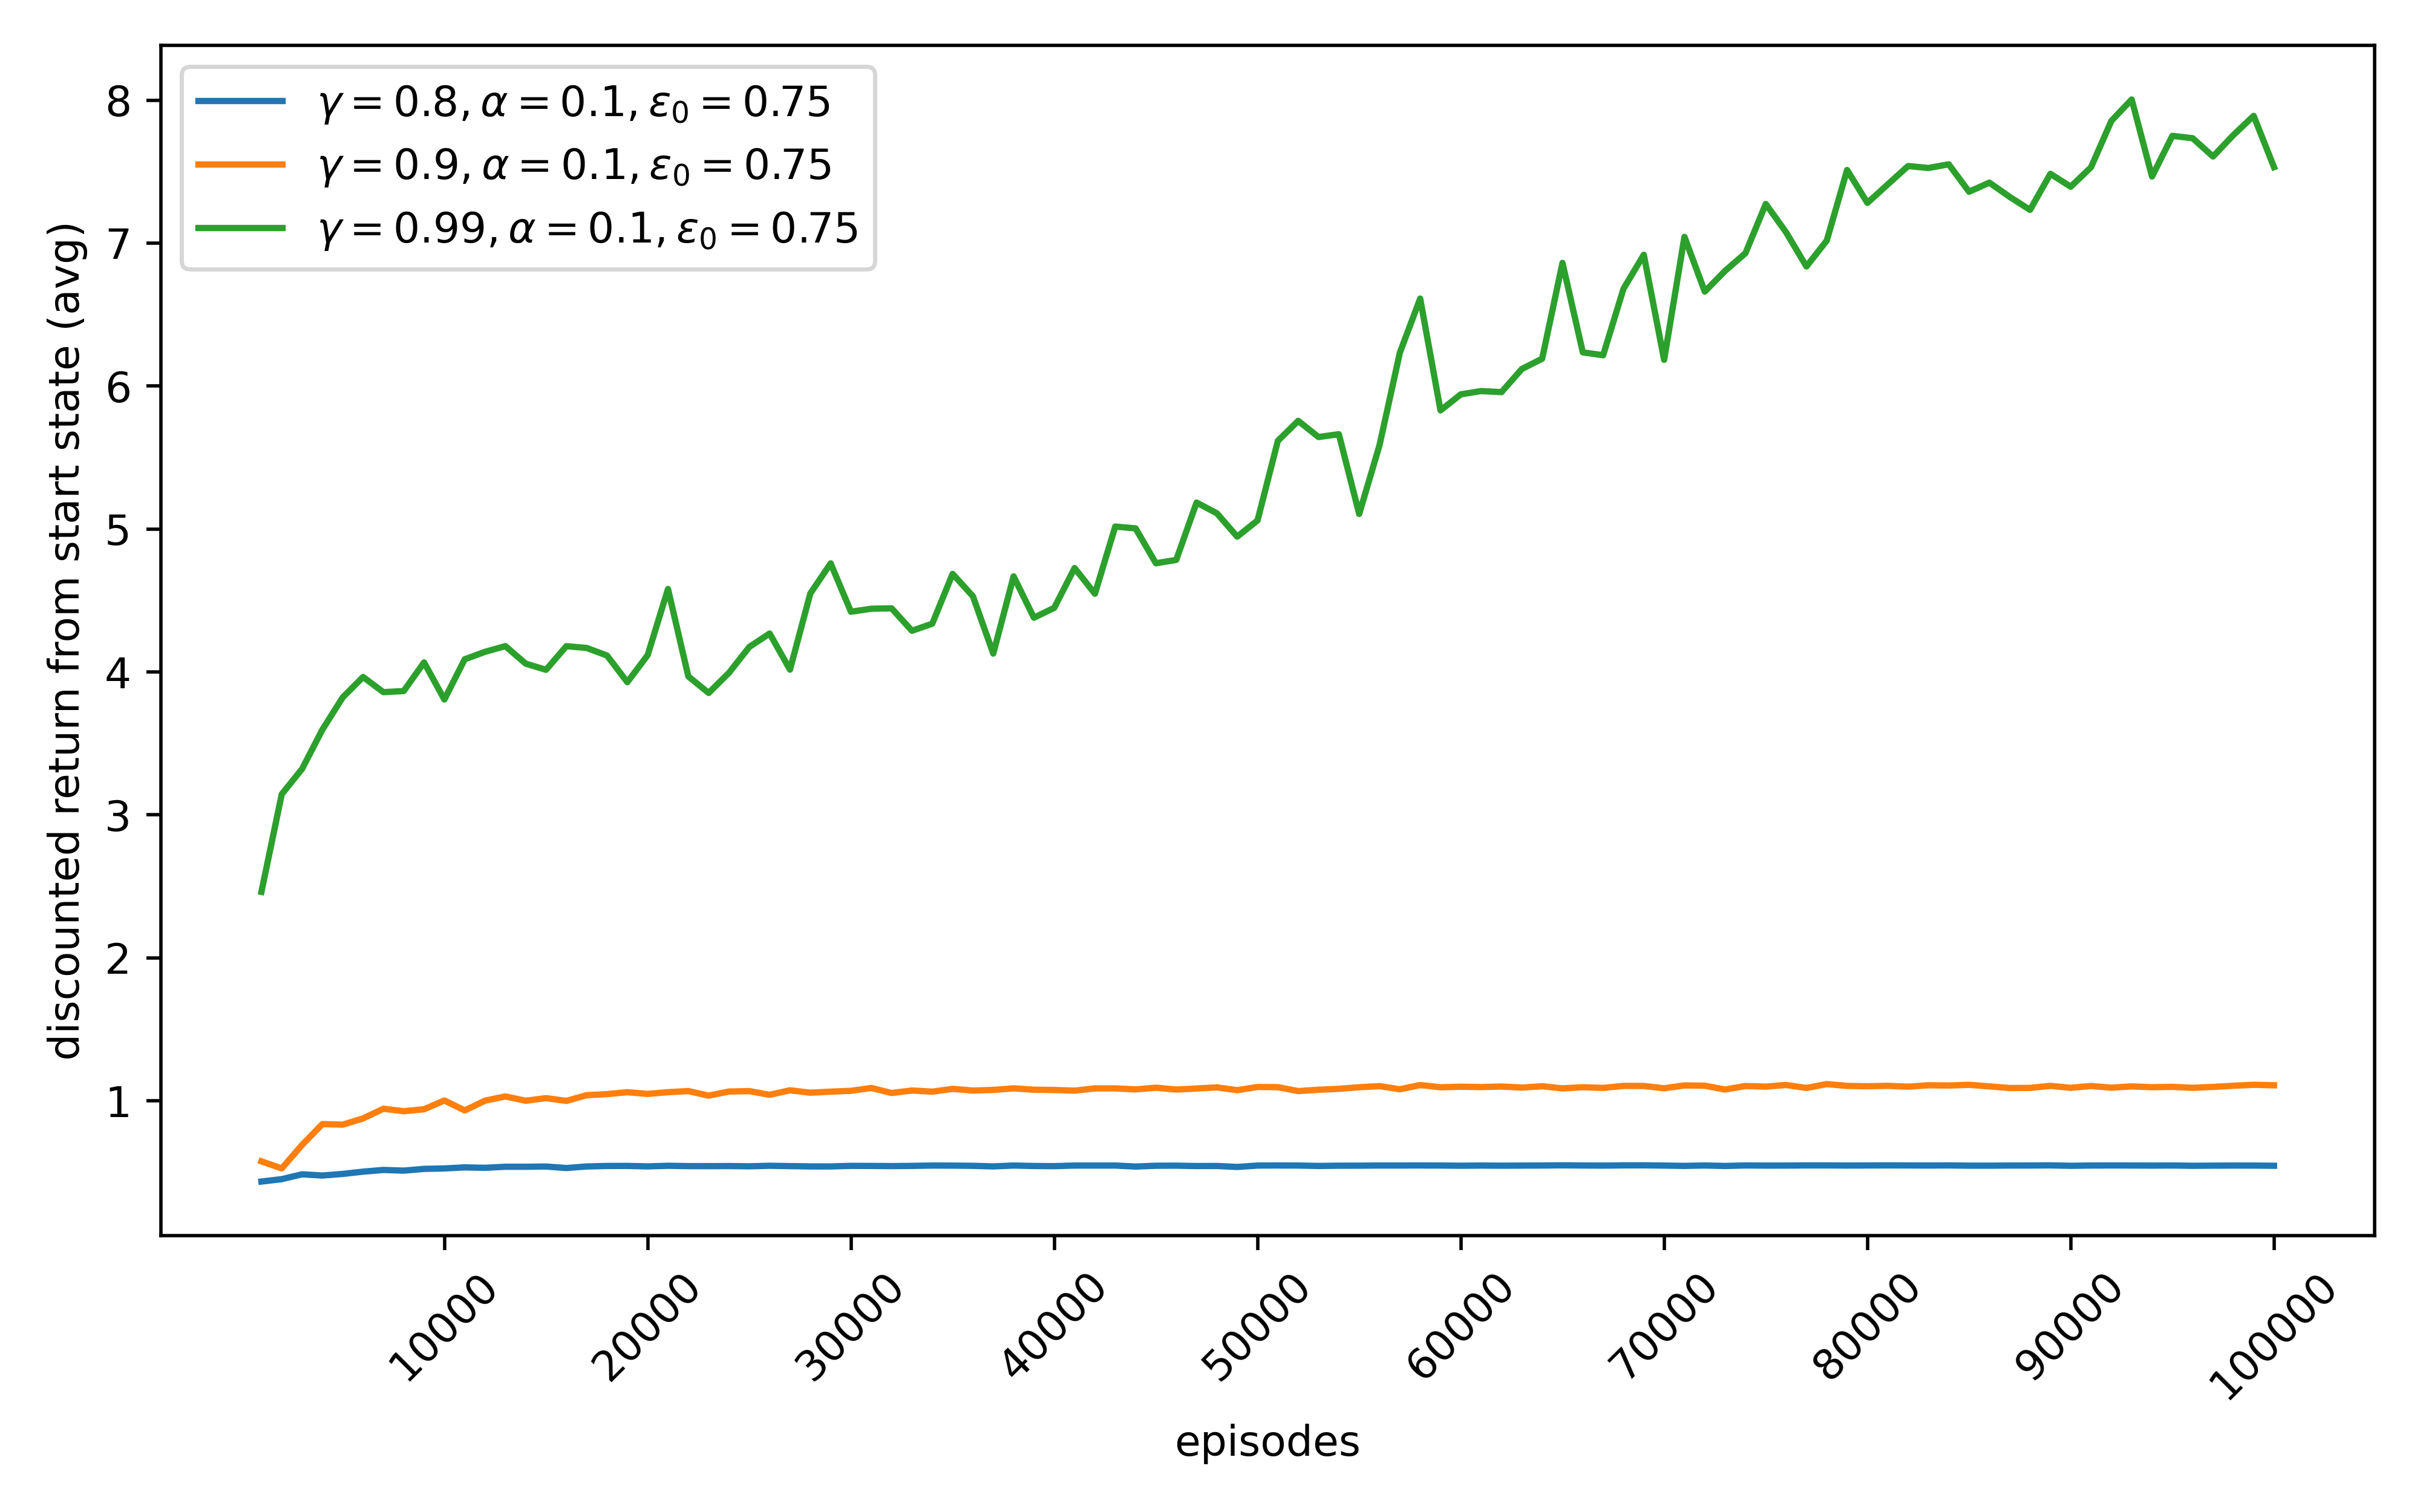
\includegraphics[width=\linewidth]{plots/part1-b-rewards.png}
        \caption{Discounted Return}
    \end{minipage}
    \hfill
    \begin{minipage}{0.49\linewidth}
        \centering
        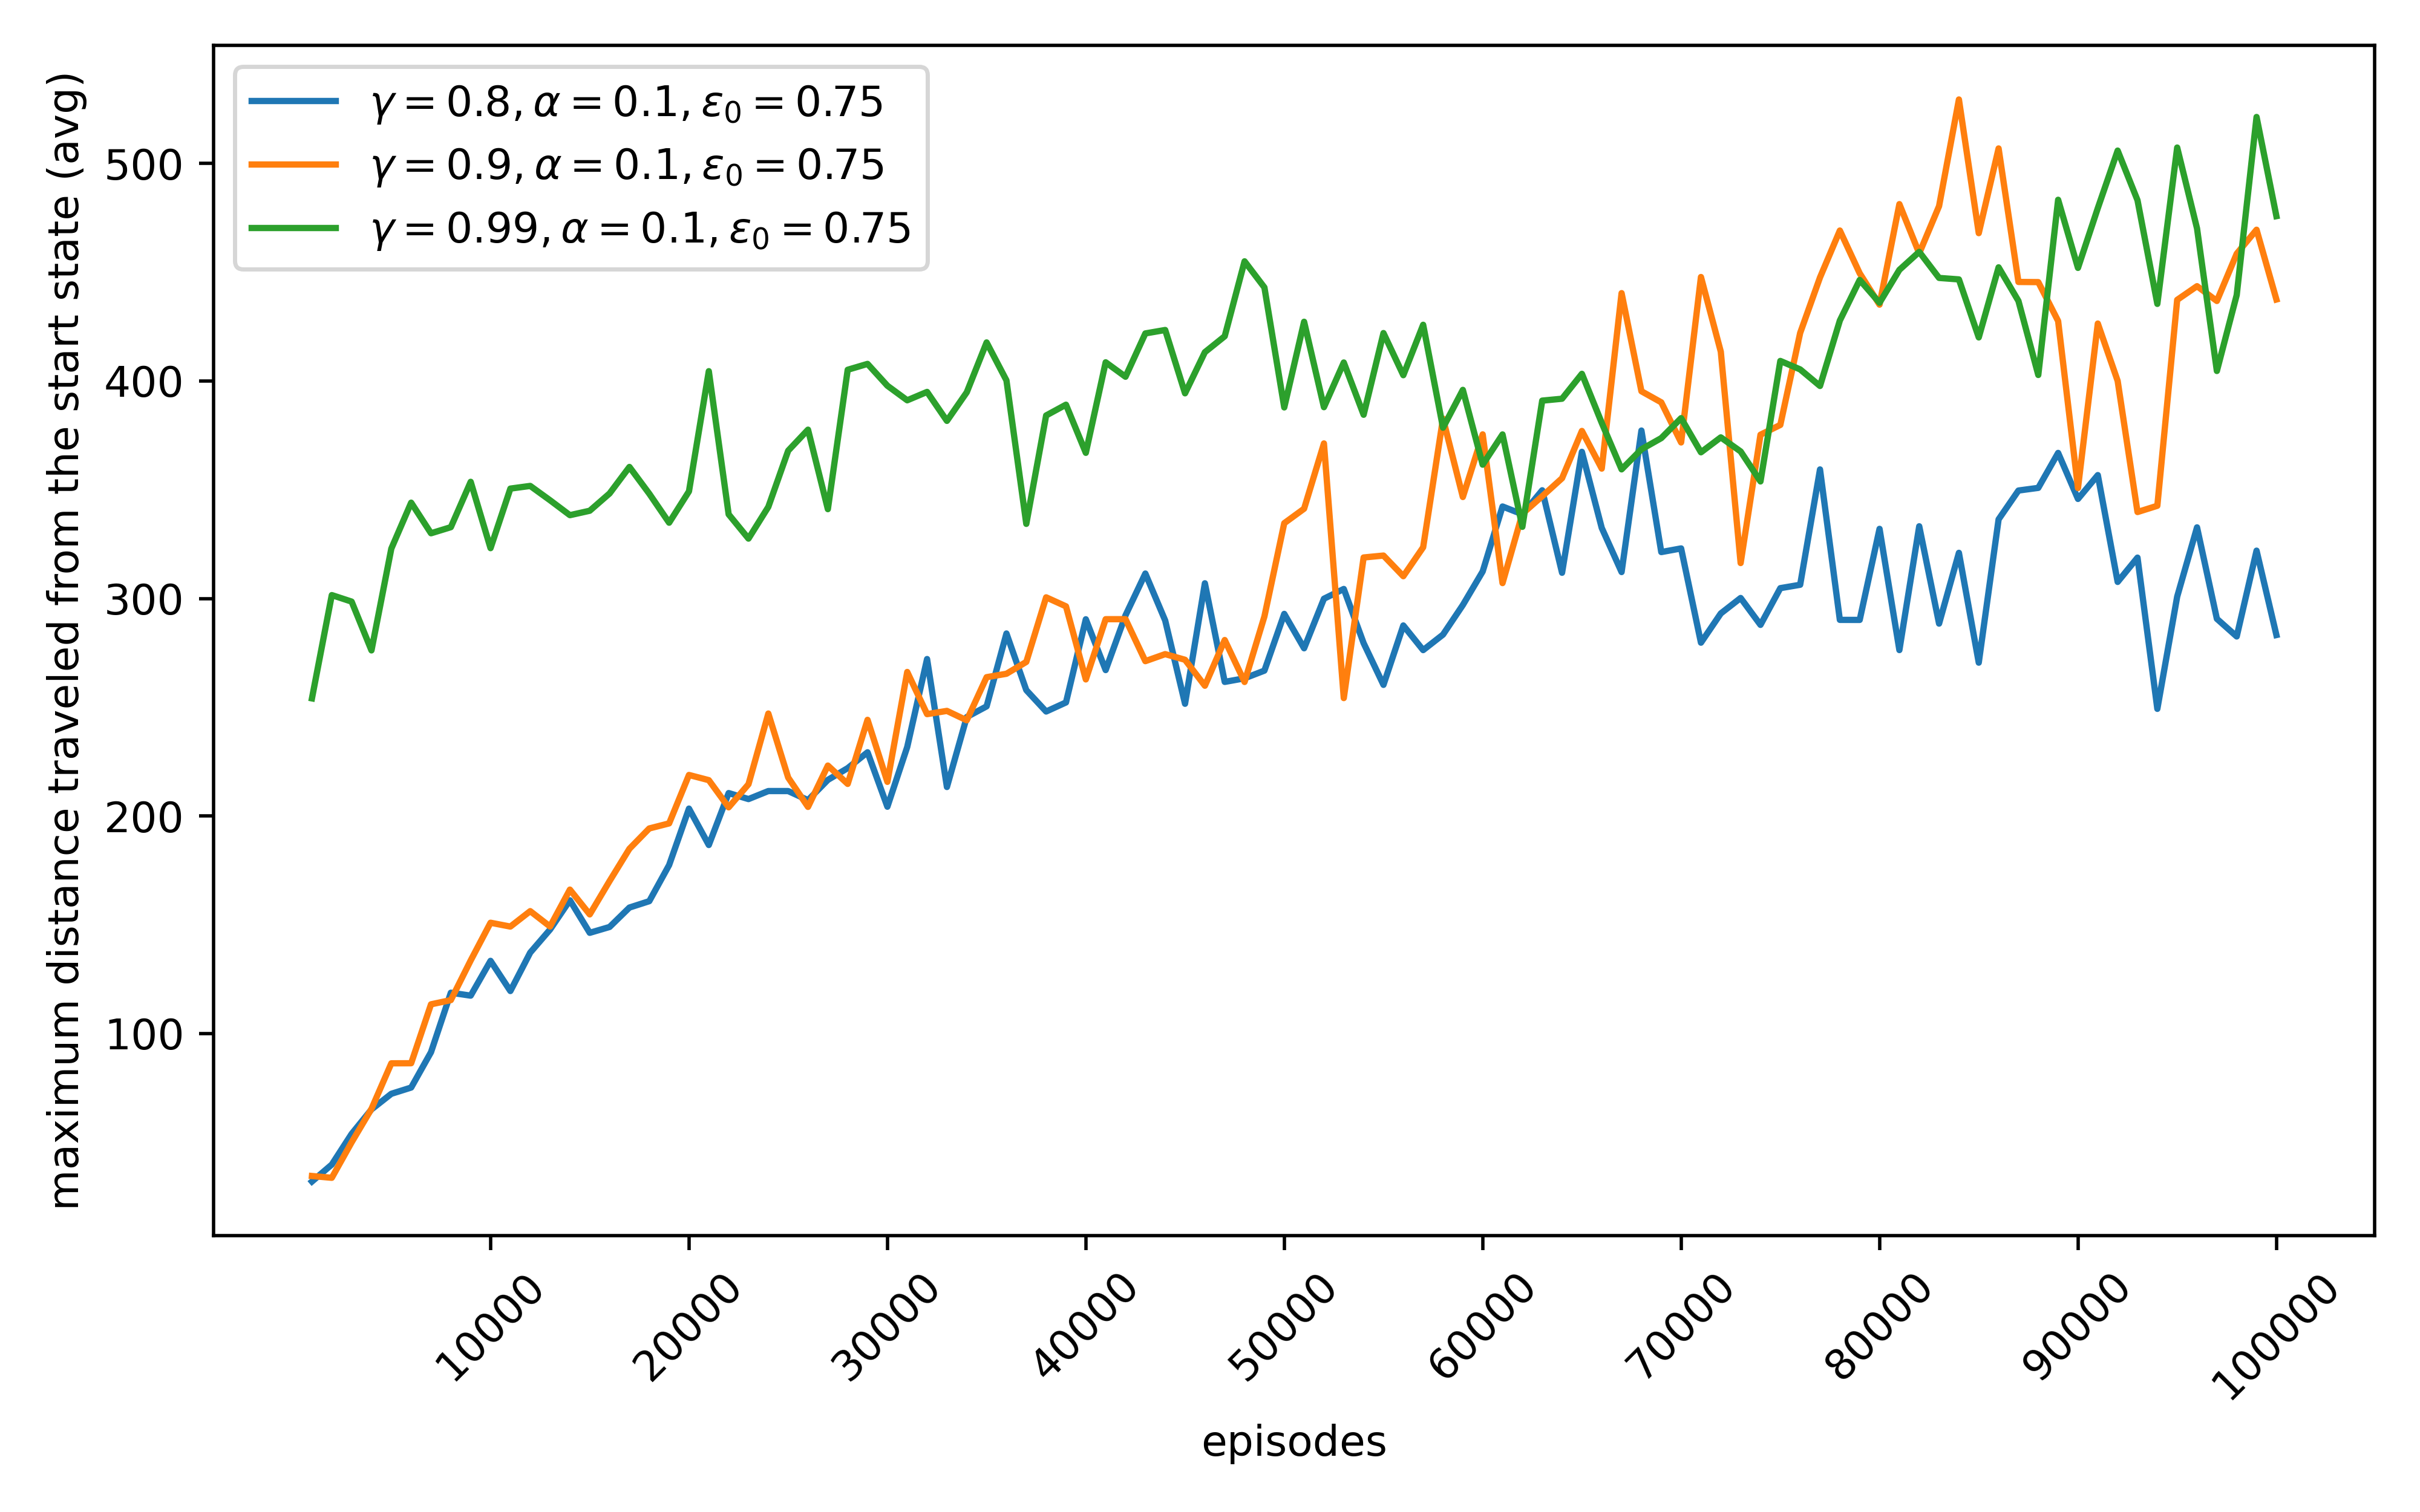
\includegraphics[width=\linewidth]{plots/part1-b-distances.png}
        \caption{Distance Traveled}
    \end{minipage}

    \vspace{1em}
    \begin{minipage}{\linewidth}
        \centering
        \begin{tabular}{lccc}
            \hline
            $\gamma$ & Discounted Return & Average Distance \\
            \hline
            $0.80$ & $0.55$ & $283.21$ \\
            $0.90$ & $1.11$ & $437.49$ \\
            $0.99$ & $7.53$ & $475.81$ \\
            \hline
        \end{tabular}
        \caption{\texttt{Tabular} $100,000$ iterations, $\alpha = 0.1, \epsilon = 0.75$}
    \end{minipage}
     \label{fig:part1-b}
\end{figure}
Increase in the discount factor tends to lead to a significant increase in the discounted returns, (as upper bound on discounted returns is $\frac{0.12}{1 - \gamma}$)  and a general increase in the average distance traveled. The reason is discussed in \nameref{sec:reward-goal}.




\subsection{Varying $\alpha$}

\begin{figure}[H]
    \centering
    \begin{minipage}{0.49\linewidth}
        \centering
        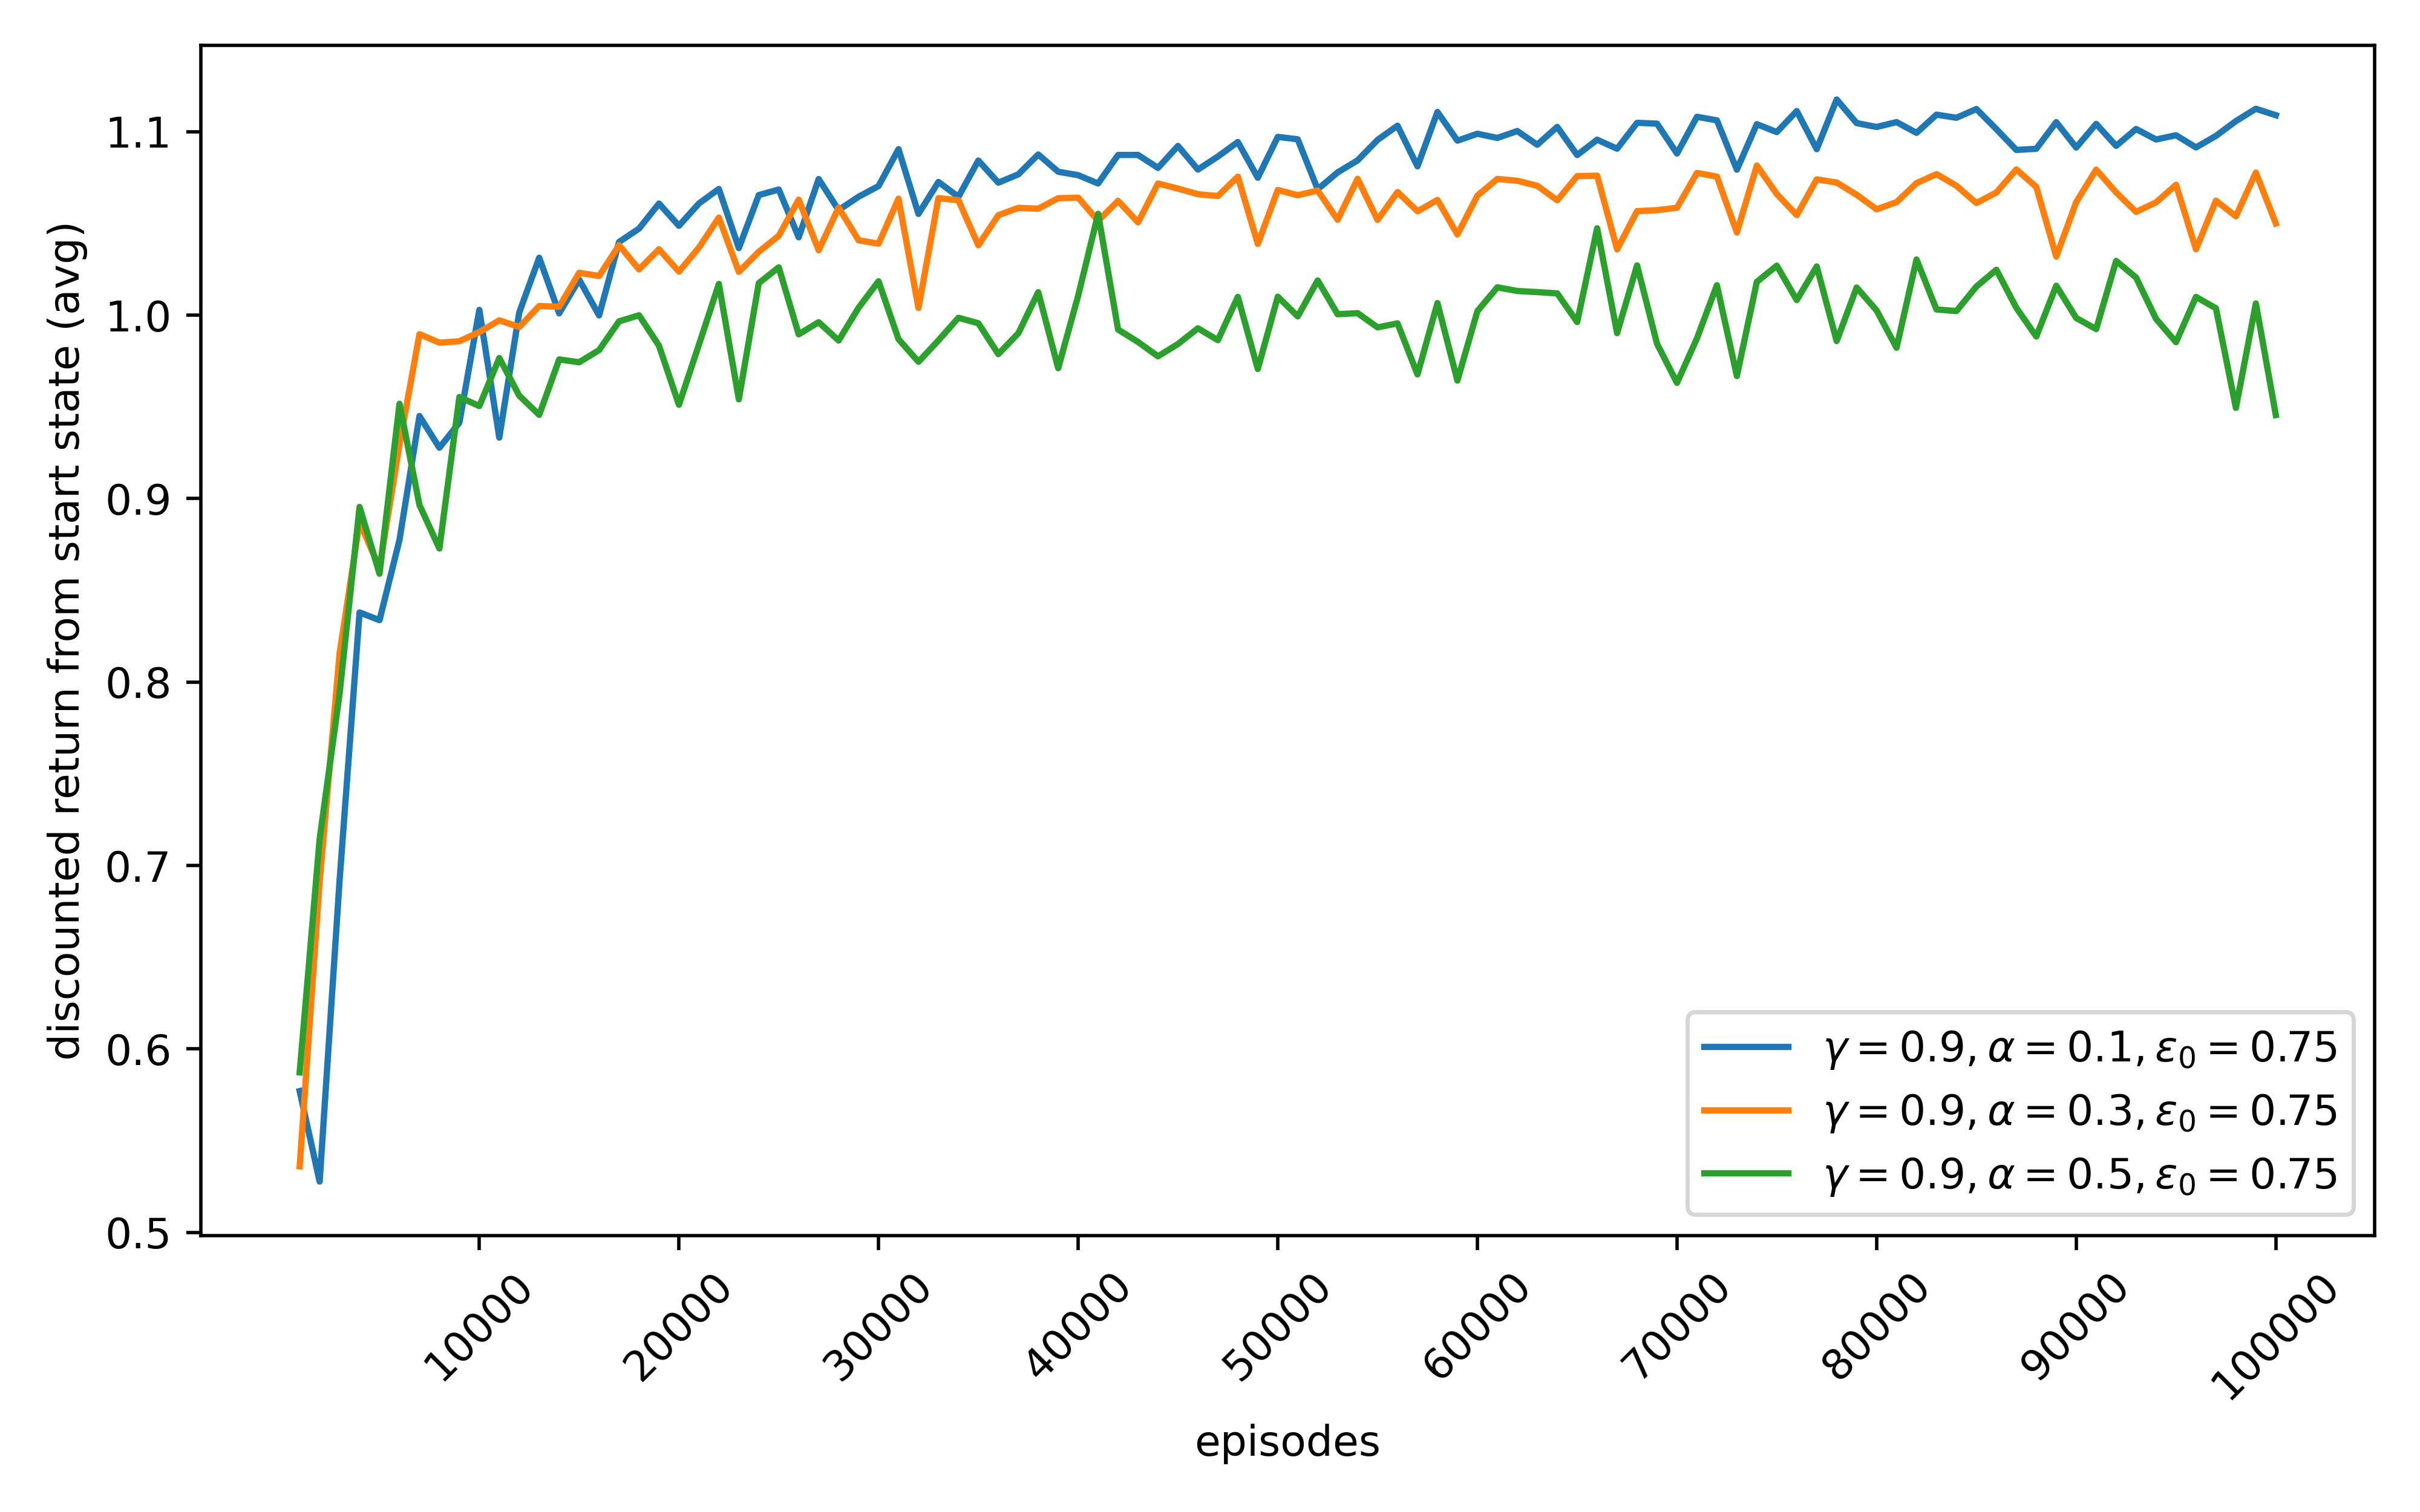
\includegraphics[width=\linewidth]{plots/part1-c-rewards.png}
        \caption{Discounted Return}
    \end{minipage}
    \hfill
    \begin{minipage}{0.49\linewidth}
        \centering
        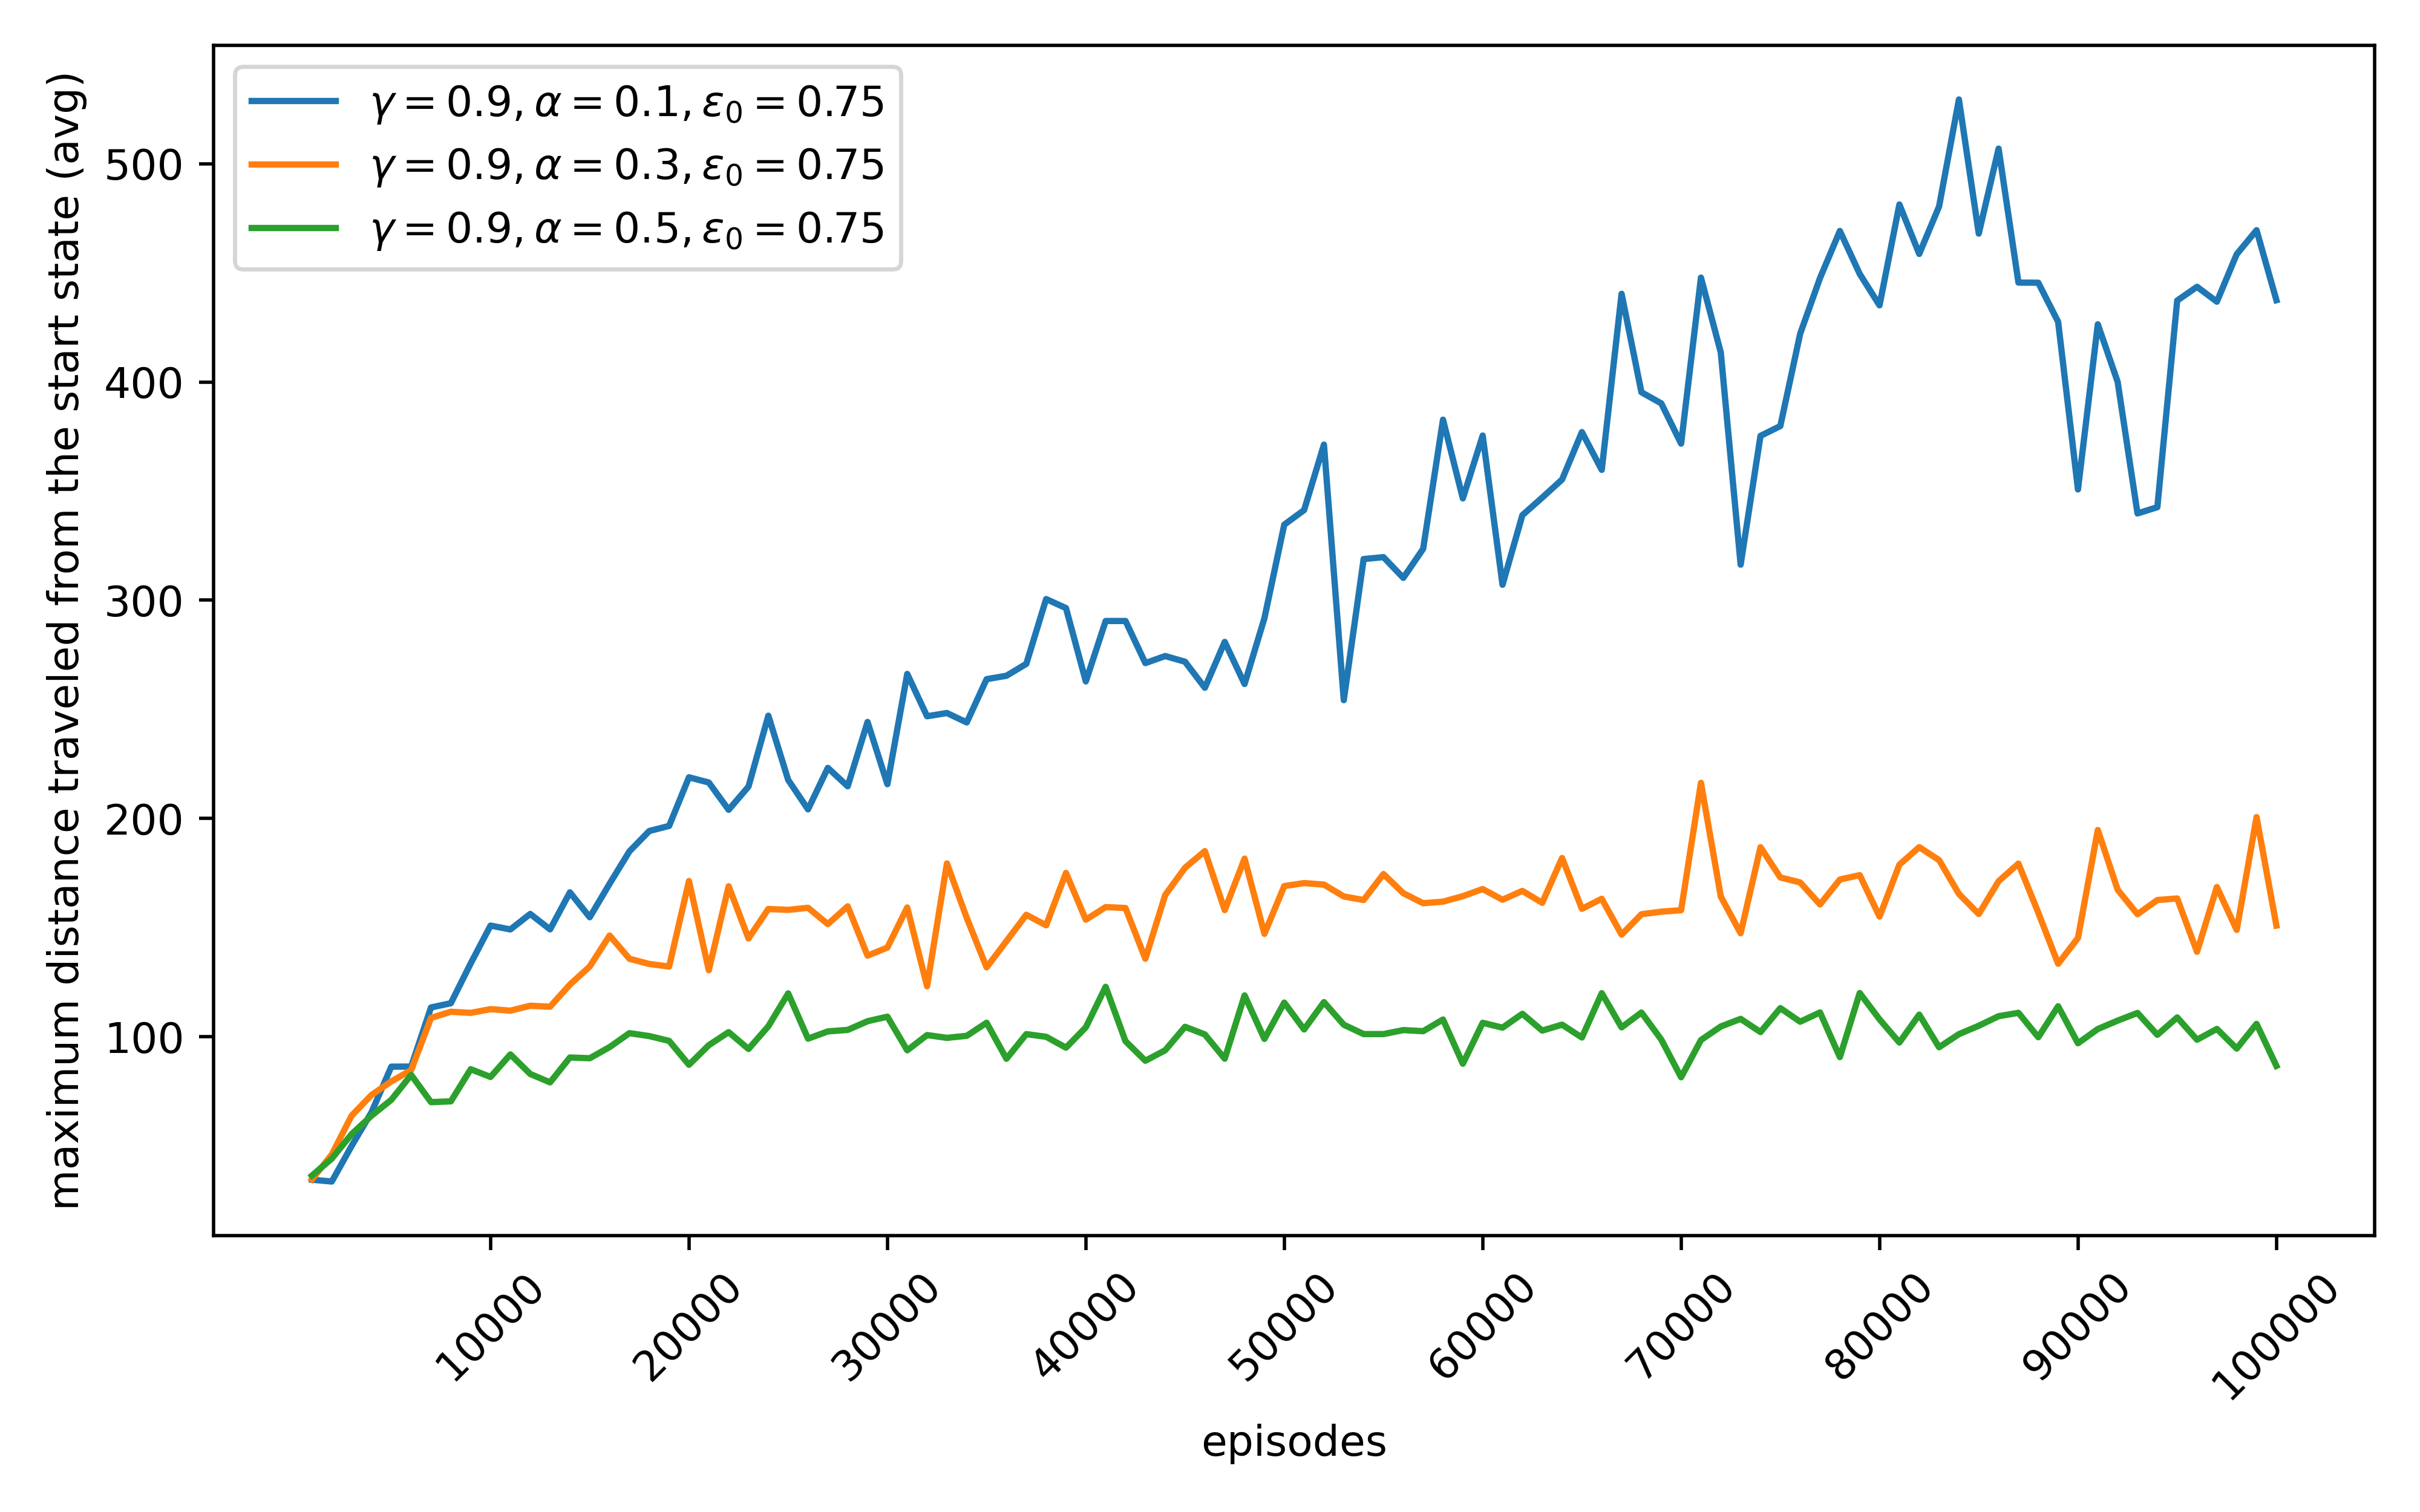
\includegraphics[width=\linewidth]{plots/part1-c-distances.png}
        \caption{Distance Traveled}
    \end{minipage}

    \vspace{1em}
    \begin{minipage}{\linewidth}
    \centering
    \begin{tabular}{lccc}
        \hline
     $\alpha$ & Discounted Return & Average Distance \\
        \hline
    $0.1$ & $1.11$ & $437.49$ \\
    $0.3$ & $1.05$ & $150.90$ \\
    $0.5$ & $0.95$ & $86.61$ \\
        \hline
    \end{tabular}
    \caption{\texttt{Tabular} $100,000$ iterations, $\gamma = 0.9, \epsilon = 0.75$} 
    \end{minipage}
     \label{fig:part1-c}
\end{figure}
In \texttt{Tabular} training, an update is made after every action. The batch size is $1$. Higher $\alpha$ means bigger updates leading to unstable training, and agent being biased towards later updates. Very briefly, during the initial few thousand episodes, higher $\alpha$ does better. Later, "forgetting" starts.


\subsection{Scheduling $\epsilon$}
\begin{figure}[H]
    \centering
    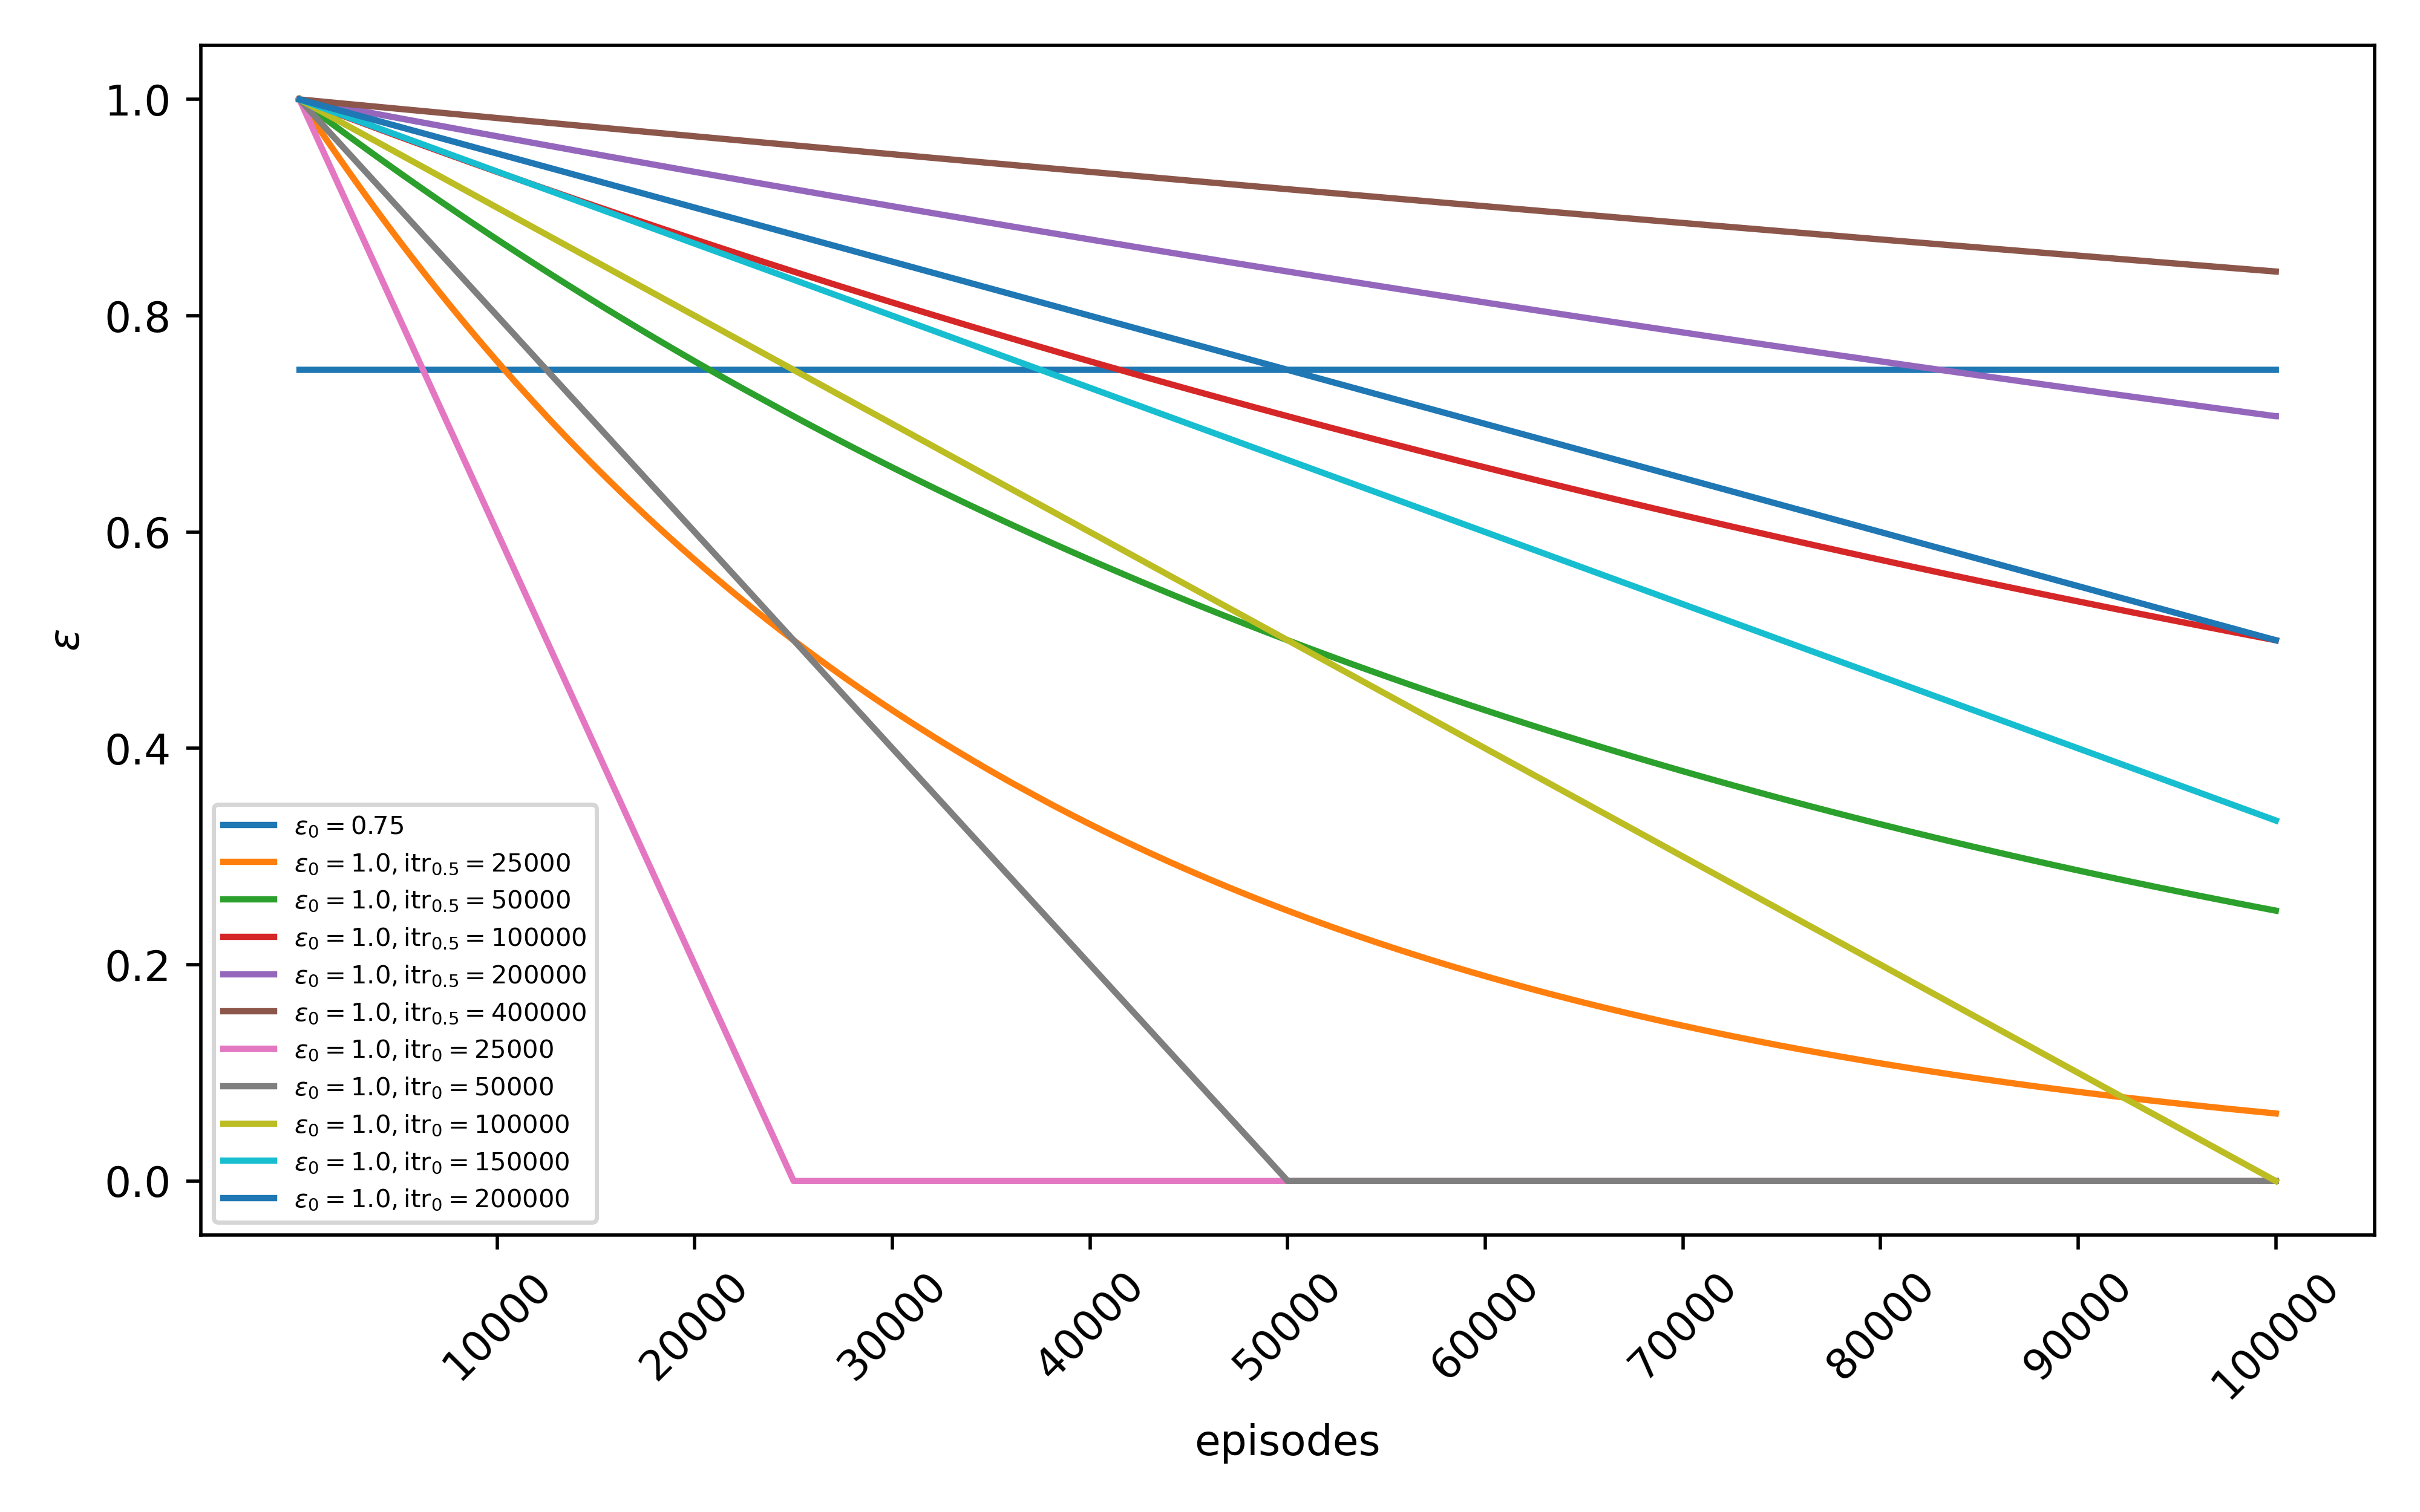
\includegraphics[width=0.5\linewidth]{plots/part1-d-epsilons.png}
    \caption{$\epsilon$ while training}
    \label{fig:part1-d-epsilons}
\end{figure}
\begin{figure}[H]
    \centering
    % First Row - Plots
    \begin{minipage}{0.32\linewidth}
        \centering
        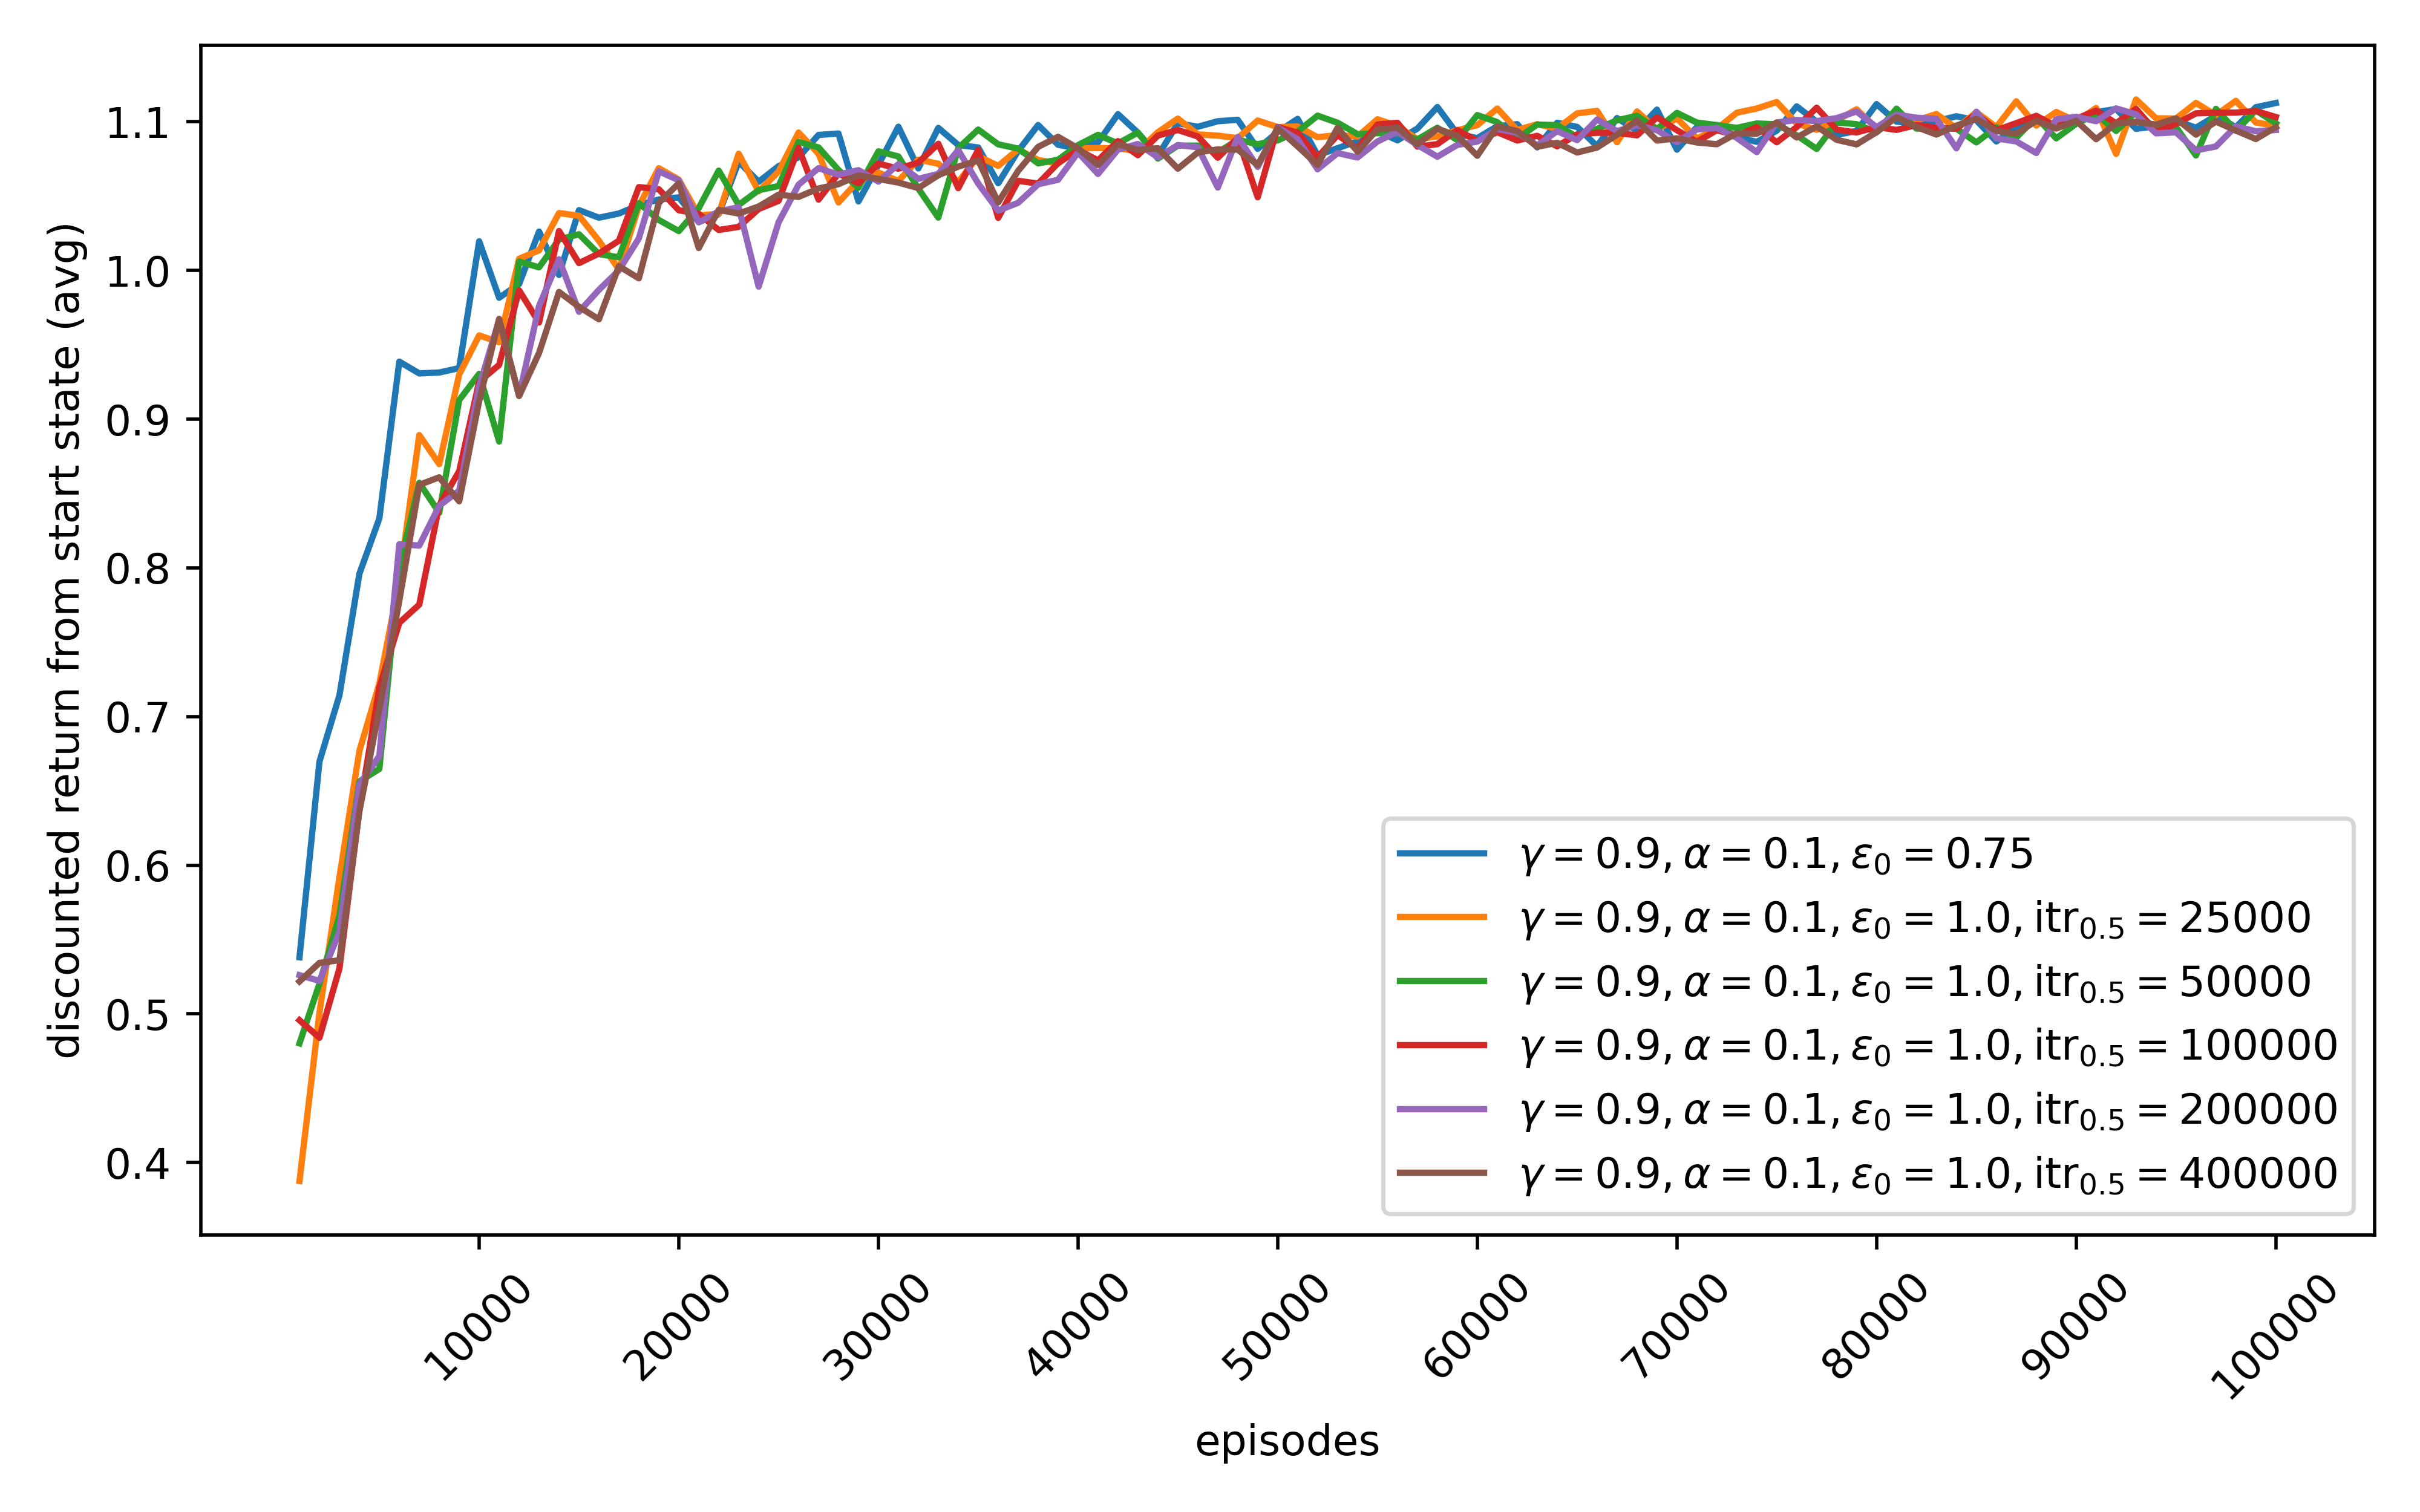
\includegraphics[width=\linewidth]{plots/part1-d.exponential-rewards.png}
        \caption{Discounted Return}
    \end{minipage}
    \hfill
    \begin{minipage}{0.32\linewidth}
        \centering
        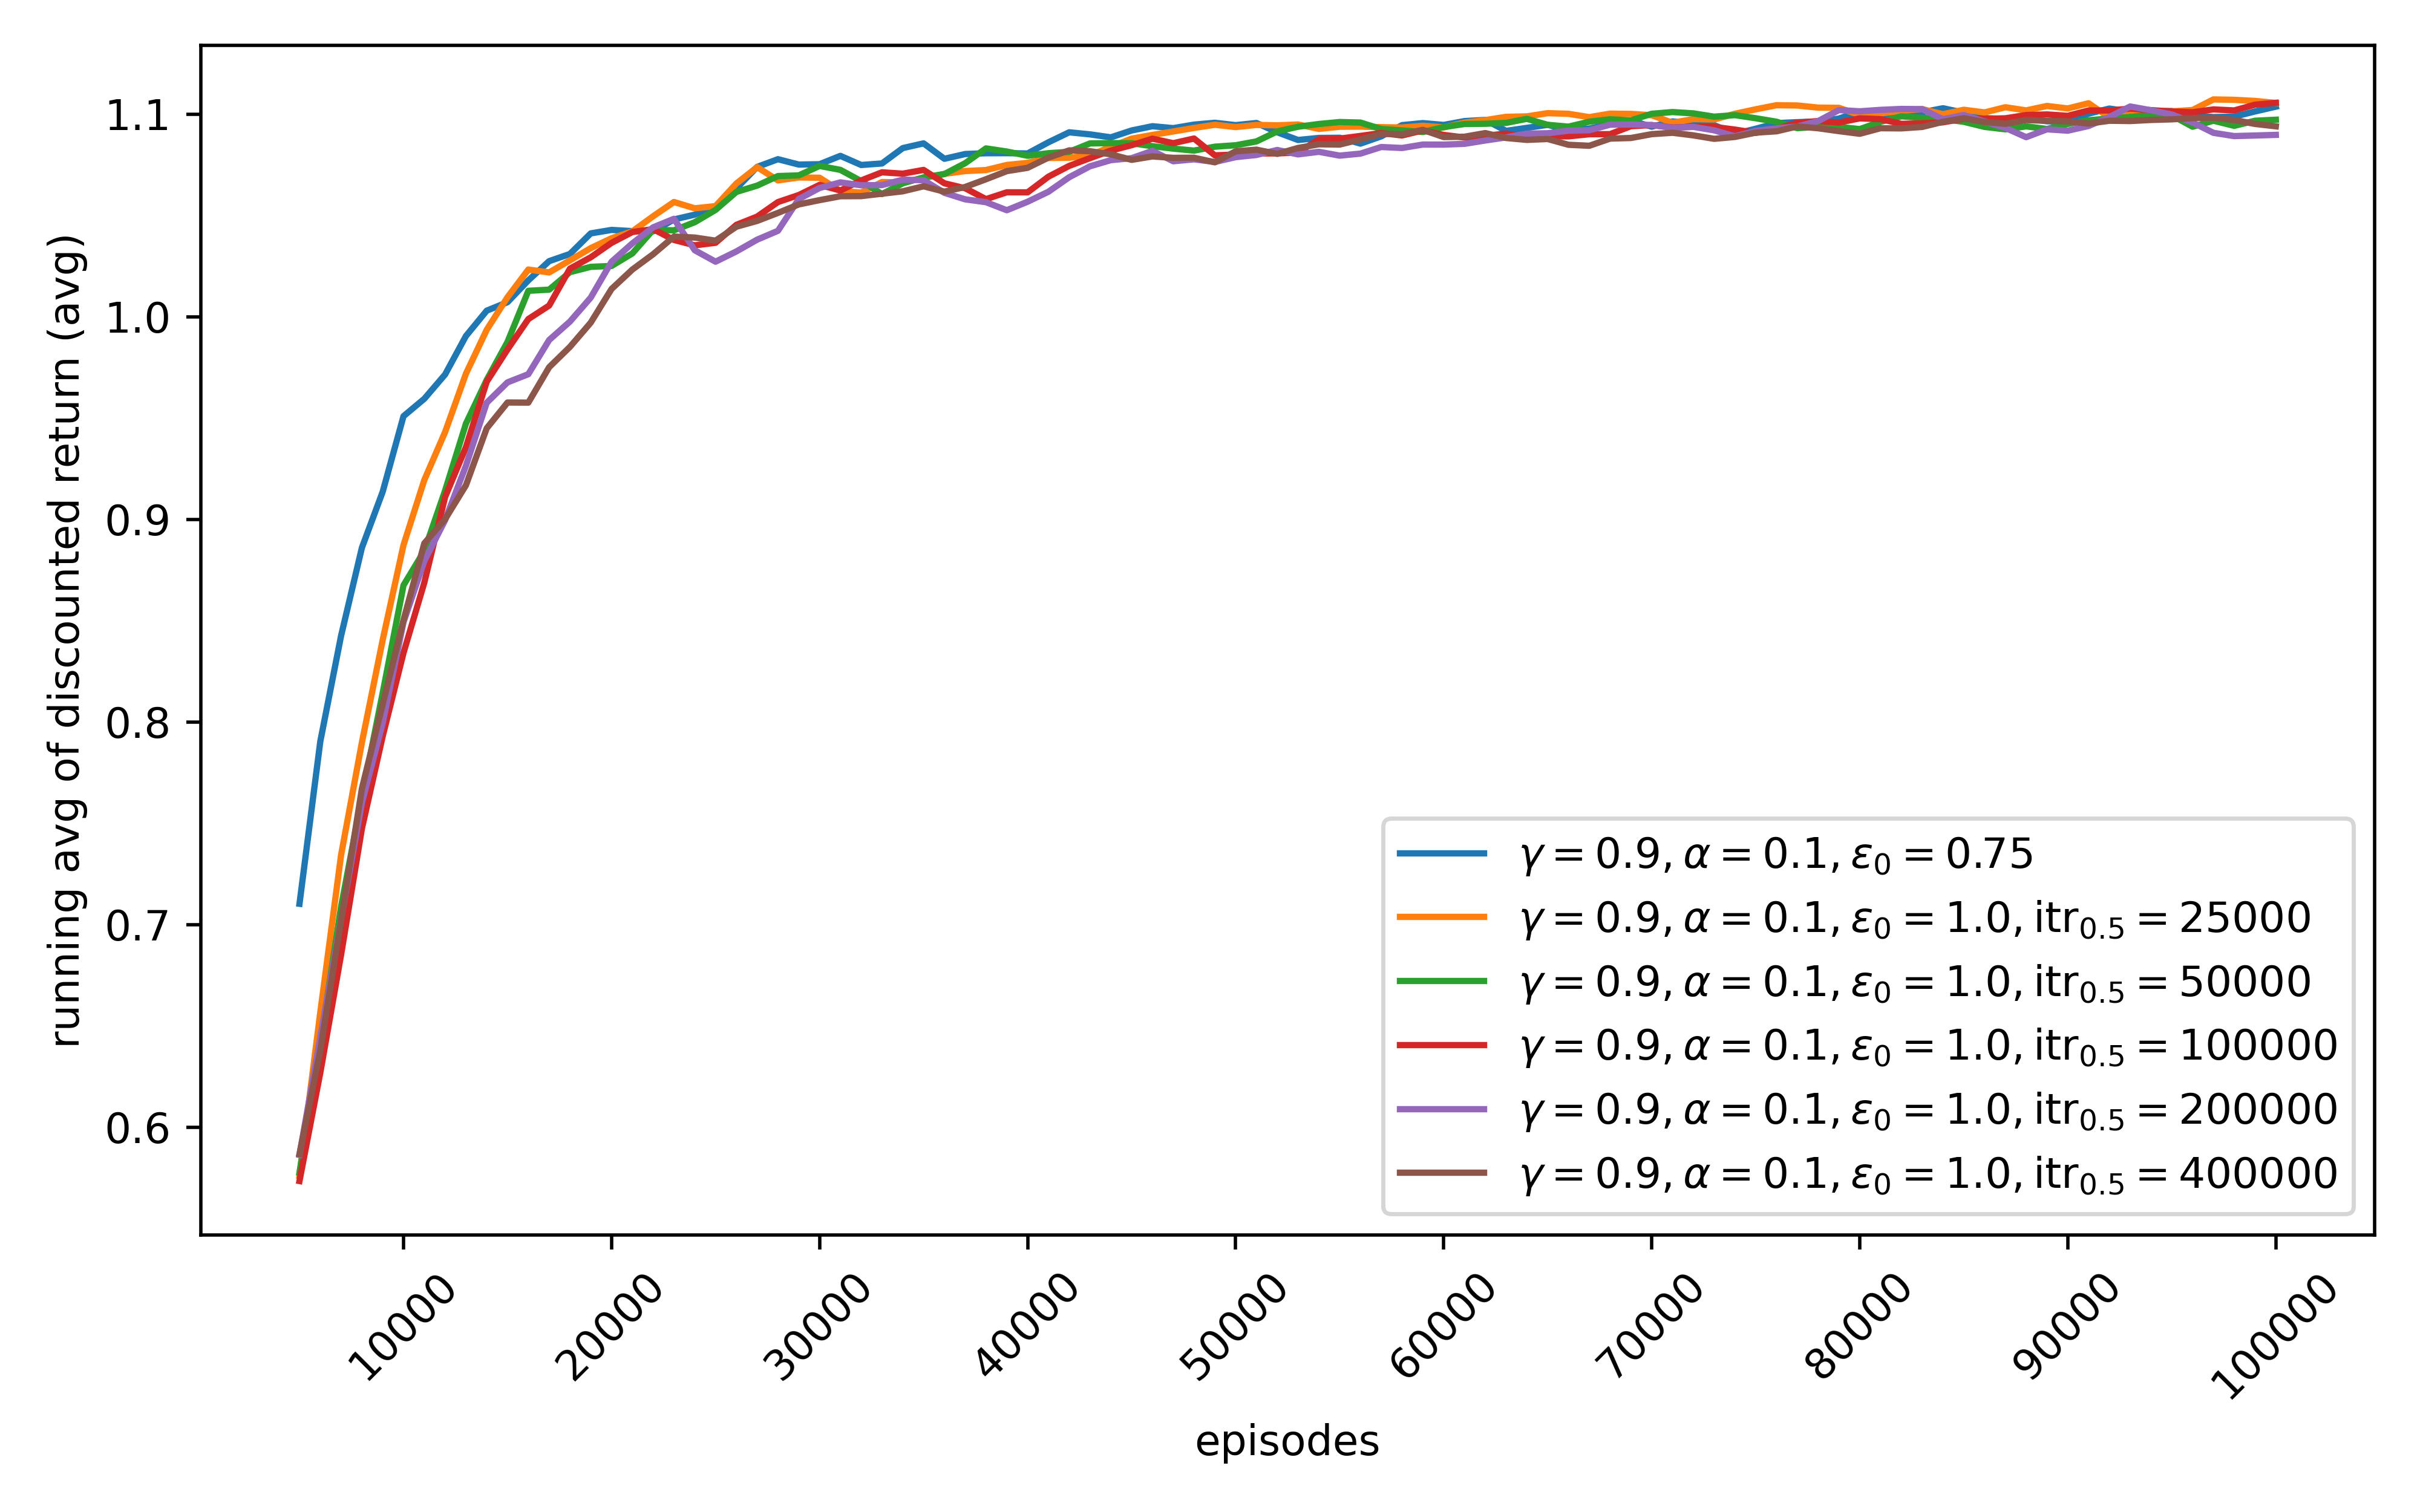
\includegraphics[width=\linewidth]{plots/part1-d.exponential-running_returns.png}
        \caption{Running Average of Discounted Return}
    \end{minipage}
    \hfill
    \begin{minipage}{0.32\linewidth}
        \centering
        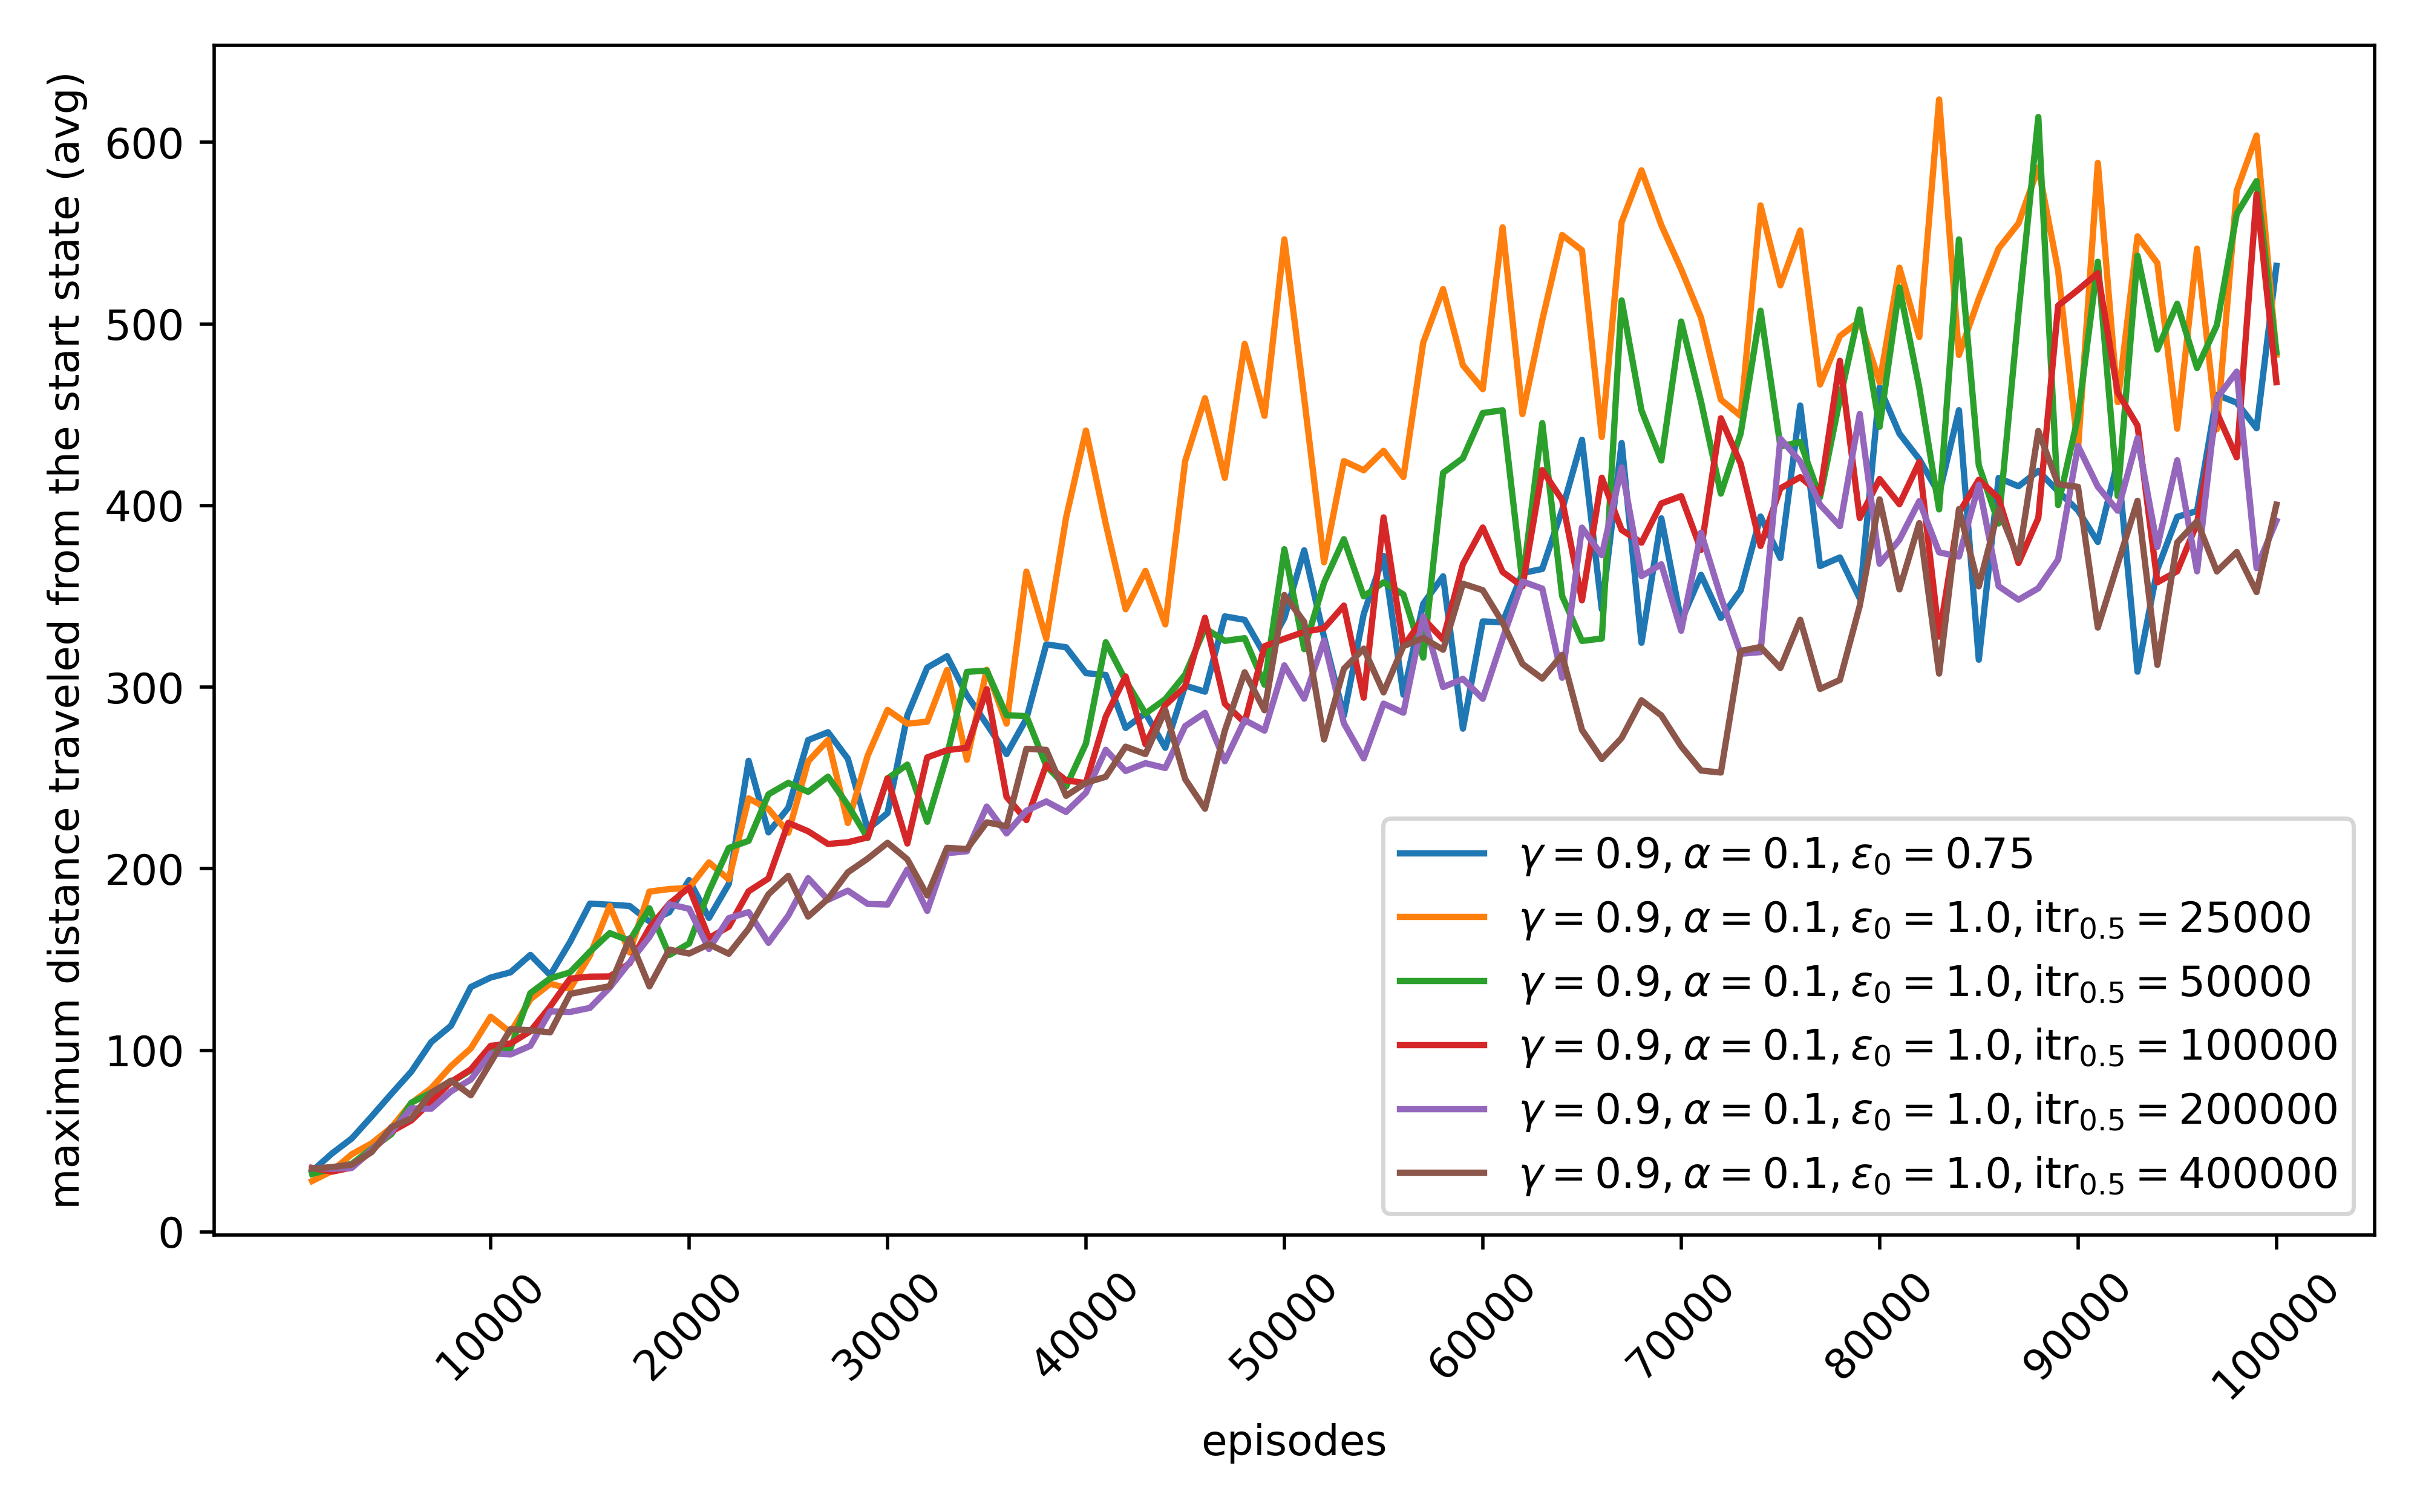
\includegraphics[width=\linewidth]{plots/part1-d.exponential-distances.png}
        \caption{Distance Traveled}
    \end{minipage}

    \vspace{0.5em}

    % Second Row - Plots
    \begin{minipage}{0.32\linewidth}
        \centering
        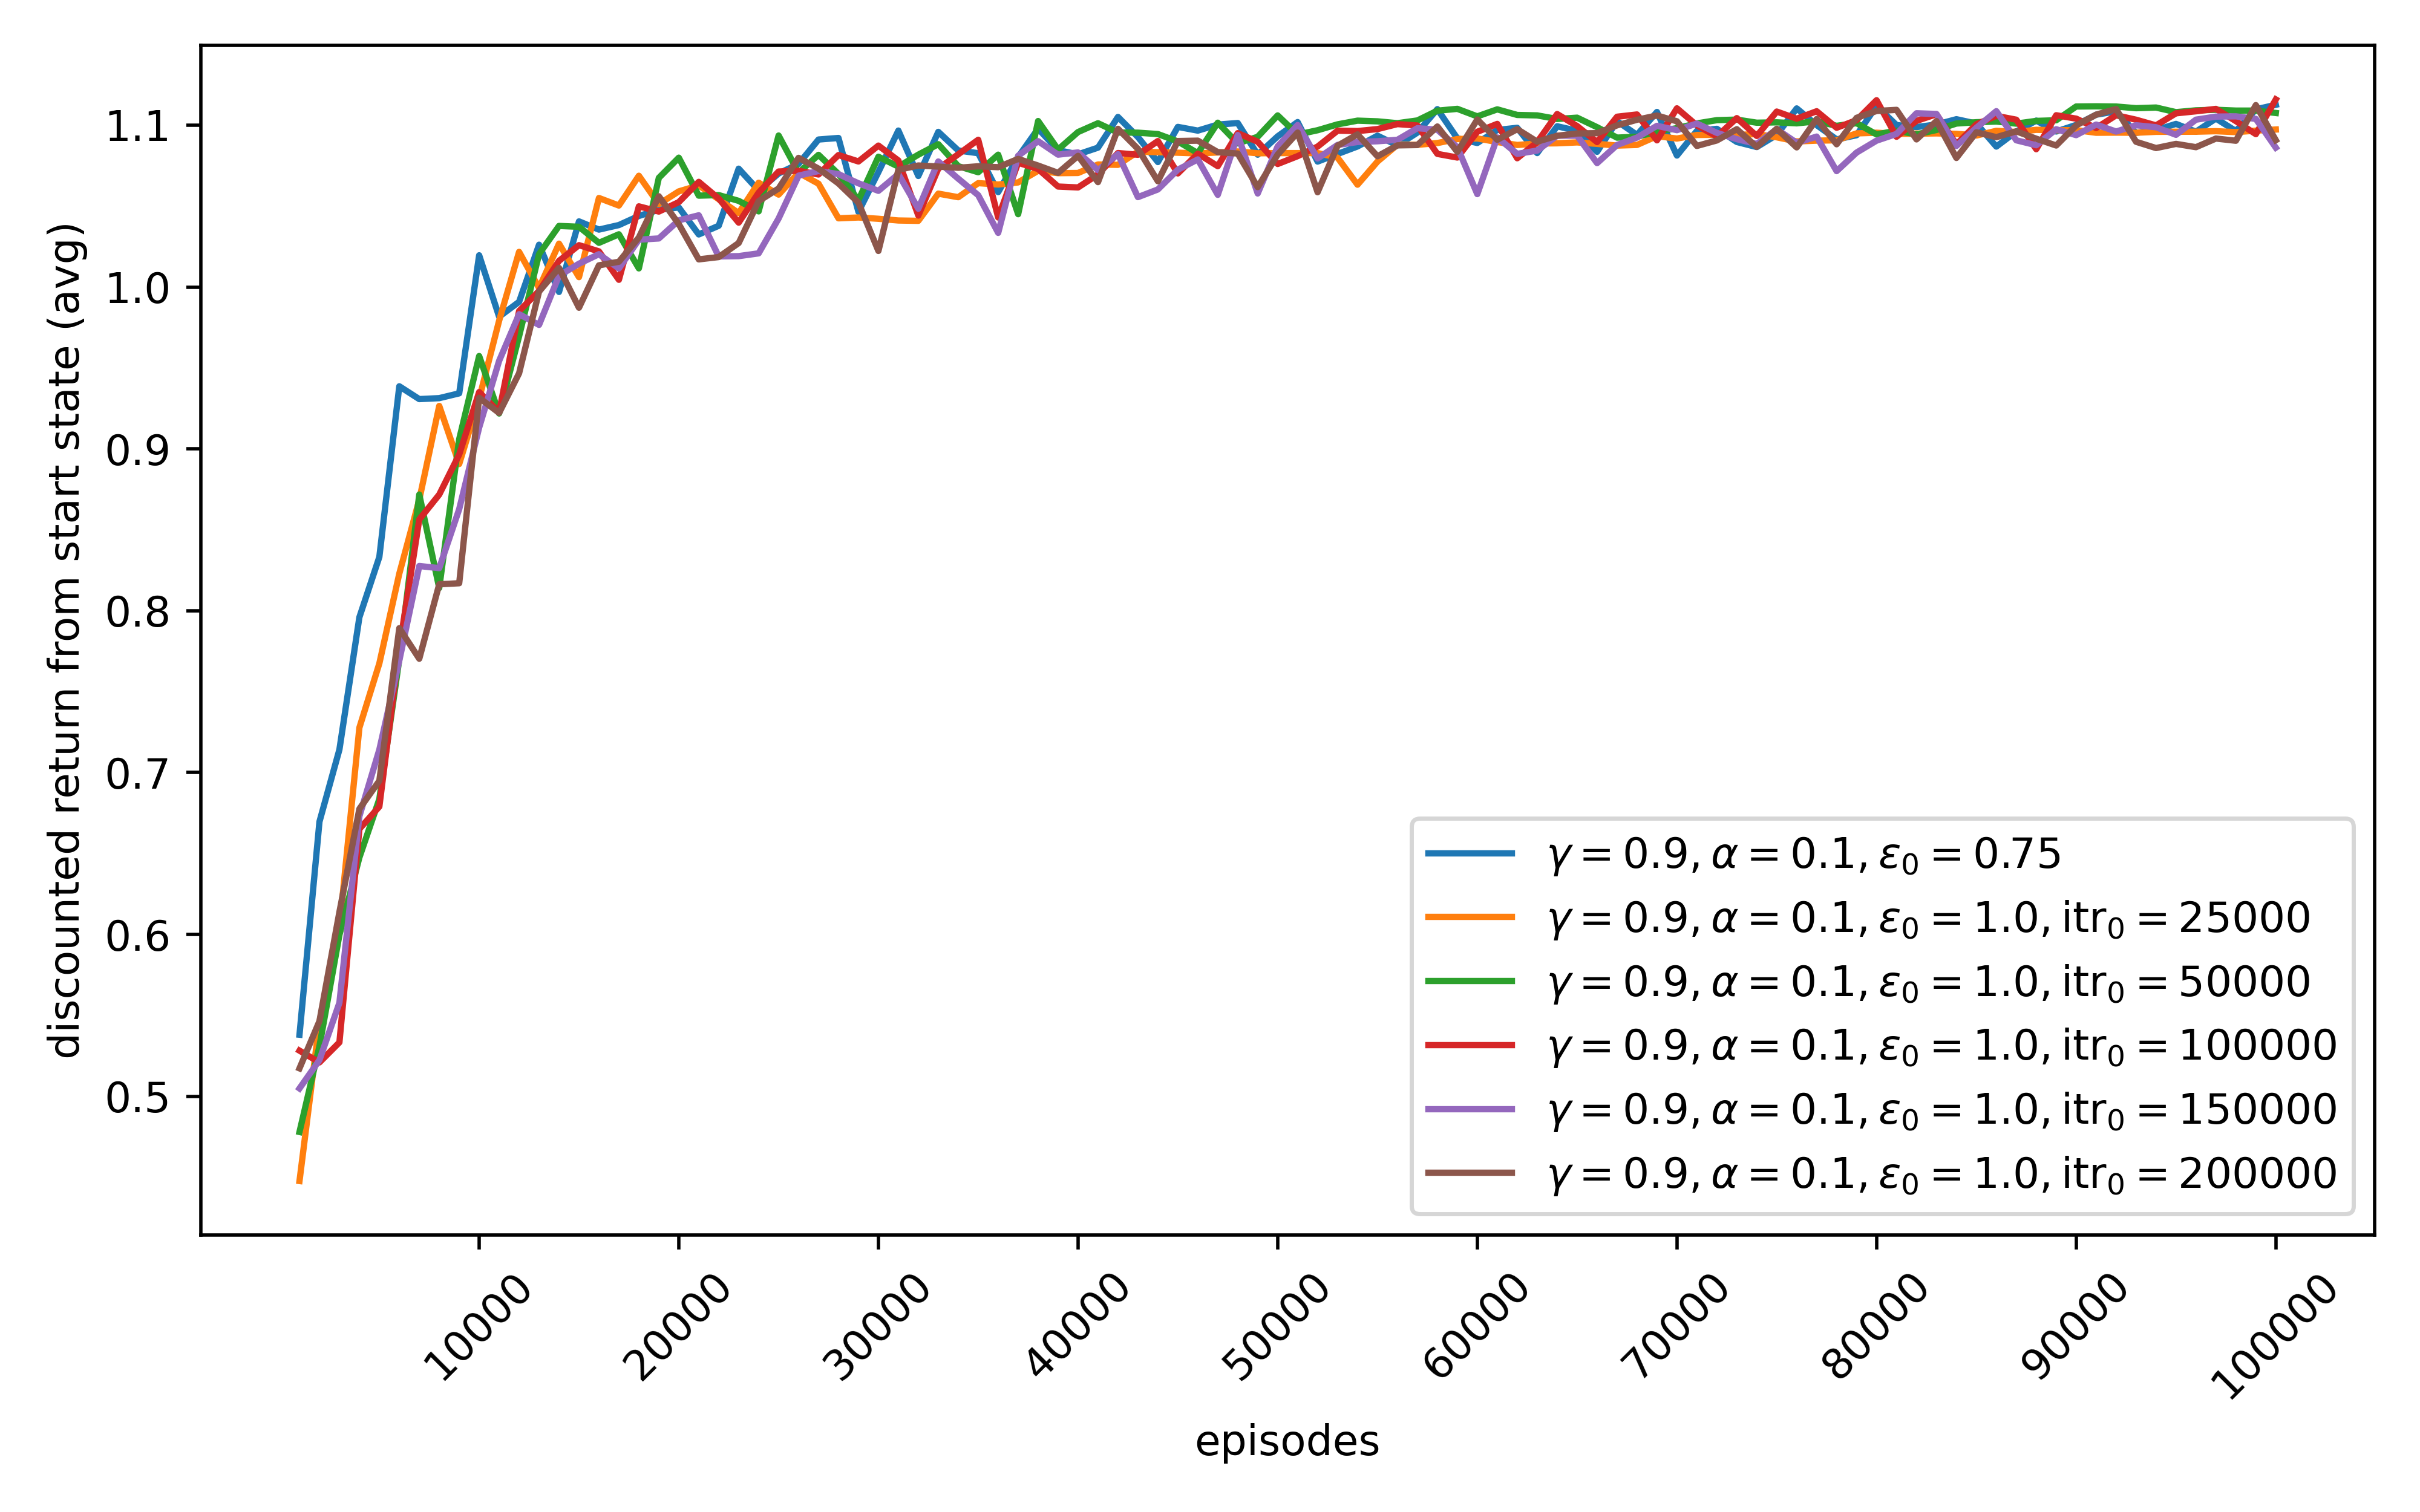
\includegraphics[width=\linewidth]{plots/part1-d.linear-rewards.png}
        \caption{Discounted Return}
    \end{minipage}
    \hfill
    \begin{minipage}{0.32\linewidth}
        \centering
        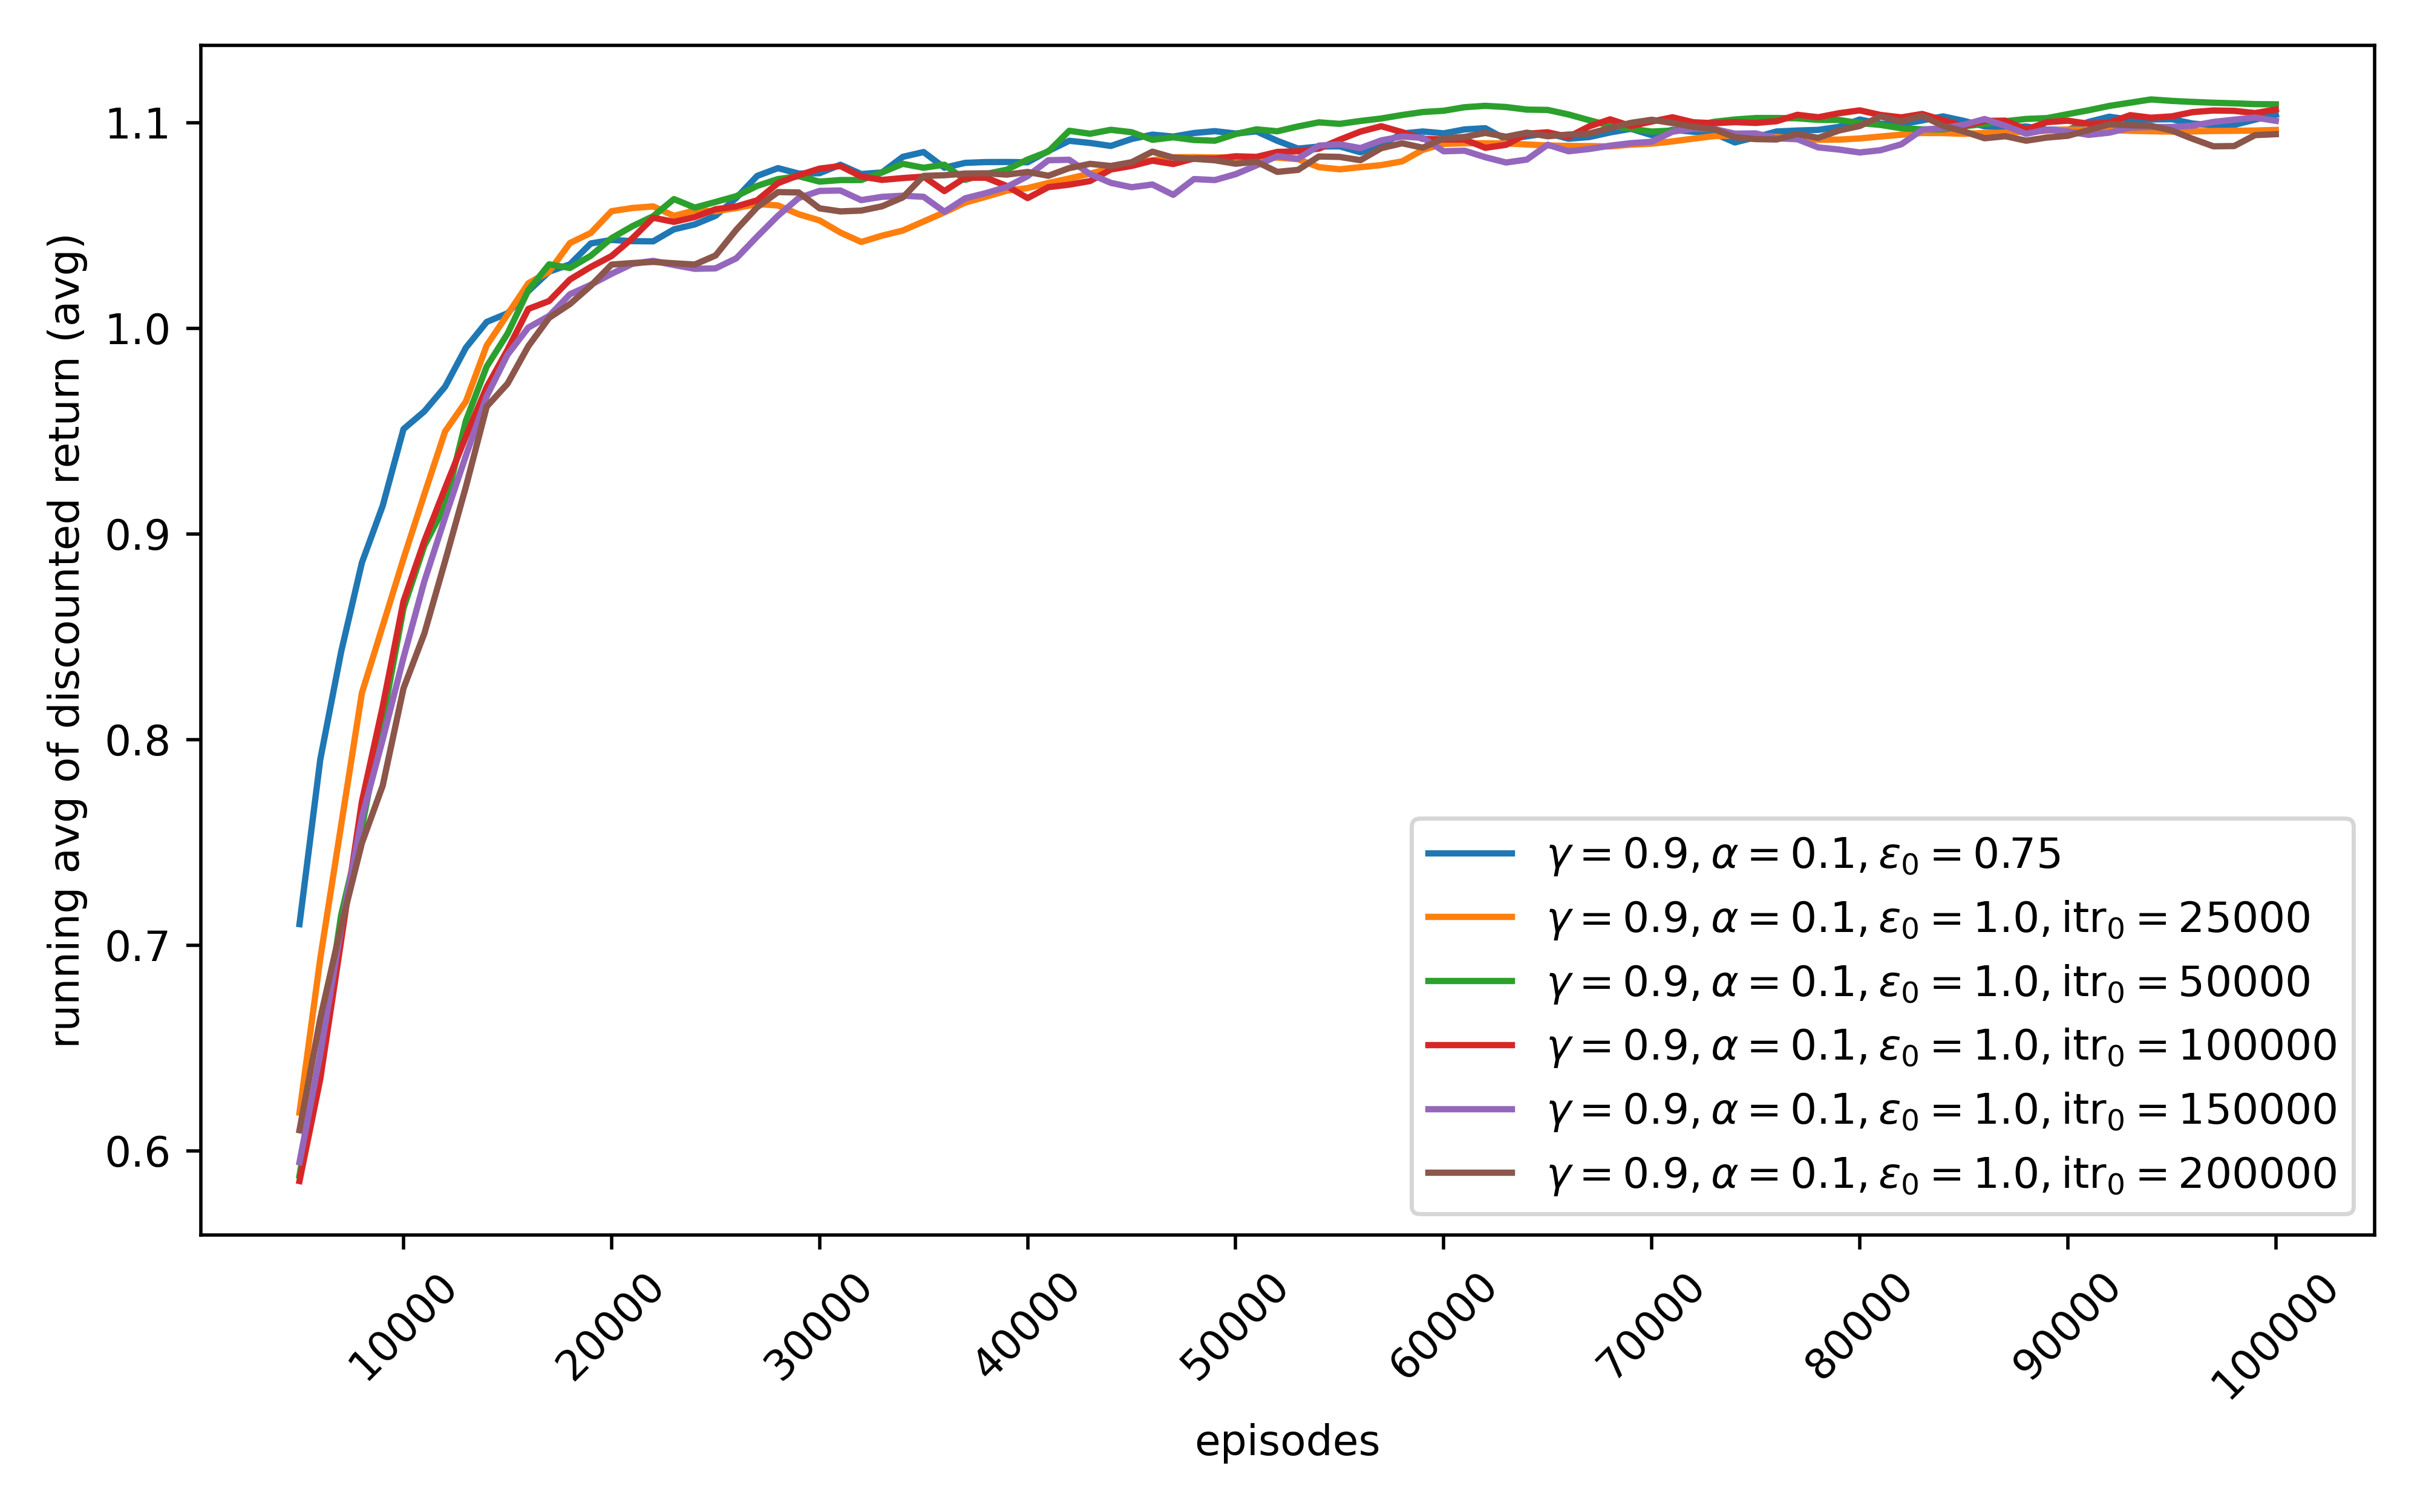
\includegraphics[width=\linewidth]{plots/part1-d.linear-running_returns.png}
        \caption{Running Average of Discounted Return}
    \end{minipage}
    \hfill
    \begin{minipage}{0.32\linewidth}
        \centering
        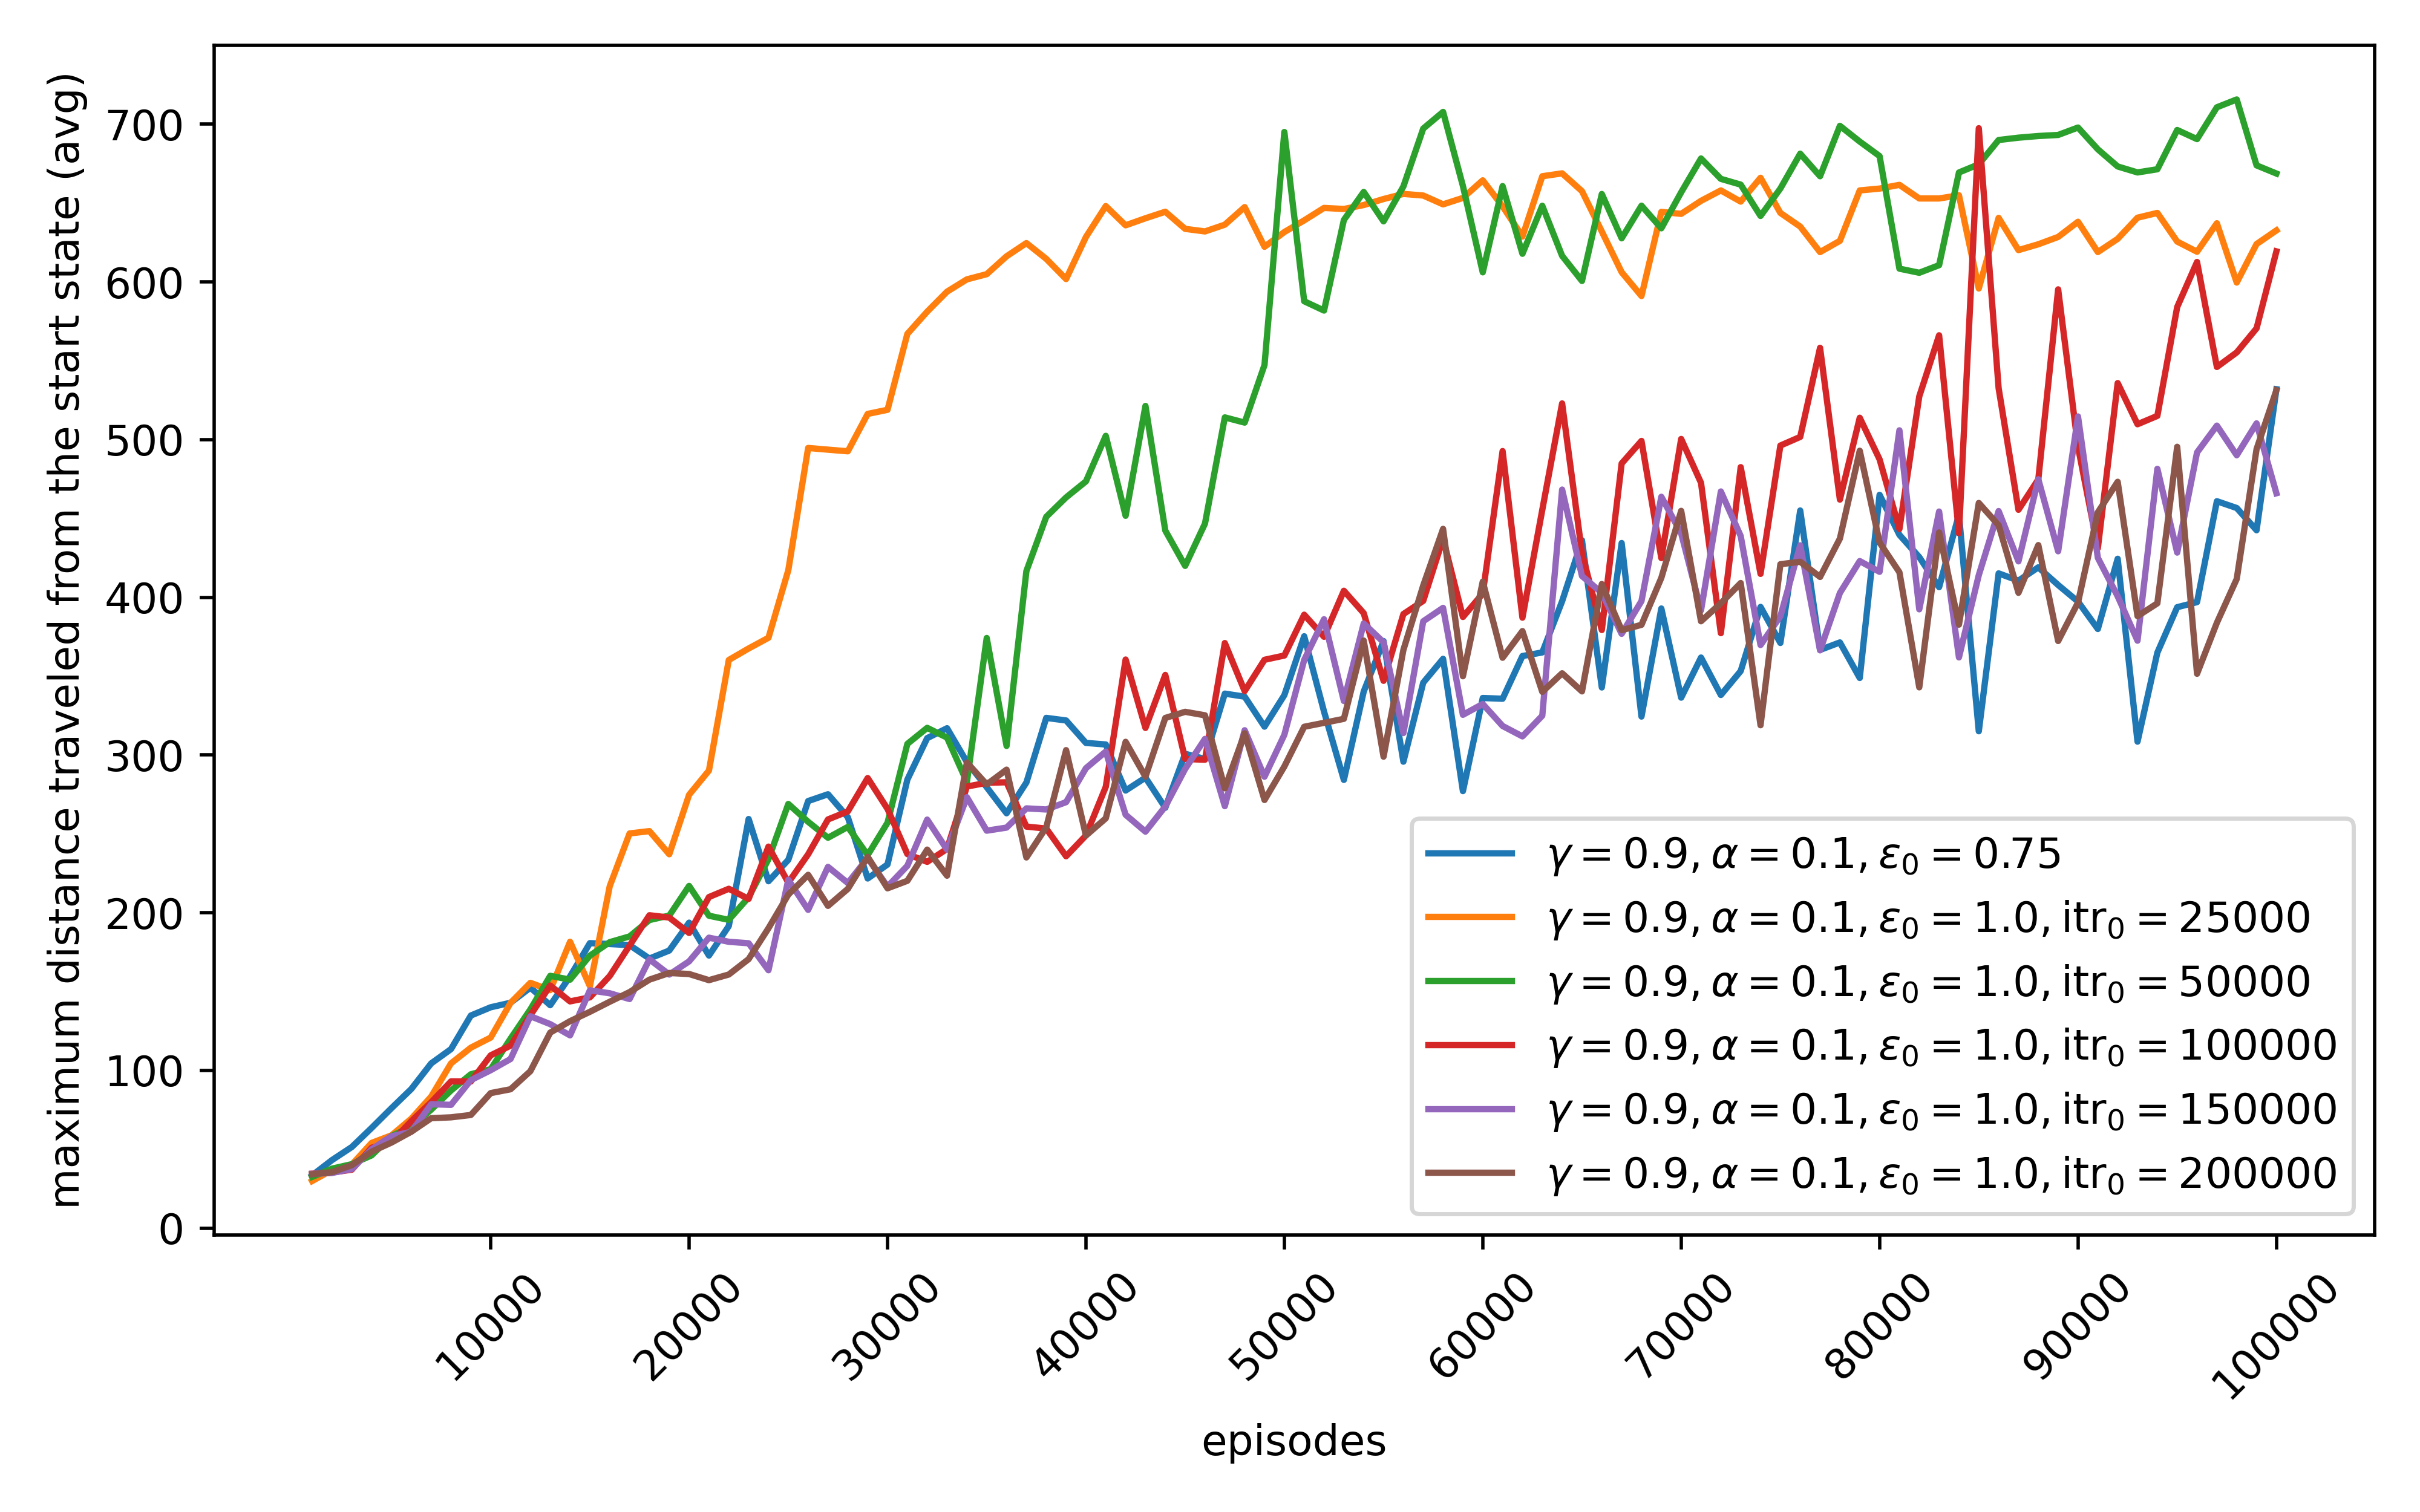
\includegraphics[width=\linewidth]{plots/part1-d.linear-distances.png}
        \caption{Distance Traveled}
    \end{minipage}
    \vspace{1em}

    % Third Row - Tables
    \begin{minipage}{0.49\linewidth}
        \centering
        \begin{tabular}{lcc}
        \hline
        $\texttt{itr}_0$ & Discounted Return & Average Distance \\
        \hline
        $25,000$ & $1.097$ & $632.68$\\ 
        $50,000$ & $1.108$ & $668.74$\\
        $100,000$ & $1.116$ & $619.39$ \\
        $150,000$ & $1.086$ & $466.01$ \\
        $200,000$ & $1.091$ & $531.35$ \\
        \hline
        \end{tabular}
        \caption{Linear Scheduling $\epsilon$}
        \label{tab:part1-d-linear}
    \end{minipage}
    \hfill
    \begin{minipage}{0.49\linewidth}
        \centering
        \begin{tabular}{lcc}
            \hline
            $\texttt{itr}_{1/2}$ & Discounted Return & Average Distance \\
            \hline
            $25,000$ & $1.097$ &  $483.09$\\
            $50,000$ & $1.099$ &  $484.38$\\
            $100,000$ & $1.103$ &  $467.94$\\
            $200,000$ & $1.094$ & $391.59$ \\
            $400,000$ & $1.096$ &  $400.47$\\
            \hline
        \end{tabular}
        \caption{Exponential Scheduling $\epsilon$}
    \end{minipage}
    \label{fig:part1-d}
    \caption{\texttt{Tabular} $100,000$ iterations, $\gamma = 0.9, \alpha = 0.1, \epsilon_0 = 1.0$} 
\end{figure}
In Linear Scheduling, Average Distance and Discounted Reward) peak at $\texttt{itr}_\texttt{0}$ $50,000$ and $100,000$ respectively. Too fast $\epsilon$ decay leads to starvation and too slow decay does not give the model enough opportunity to lean the optimum policy, given the knowledge of rewards explored. 


\section{Changing Environment}
\subsection{Overtake Reward}

\begin{figure}[H]
    \centering
    \begin{minipage}{0.49\linewidth}
        \centering
        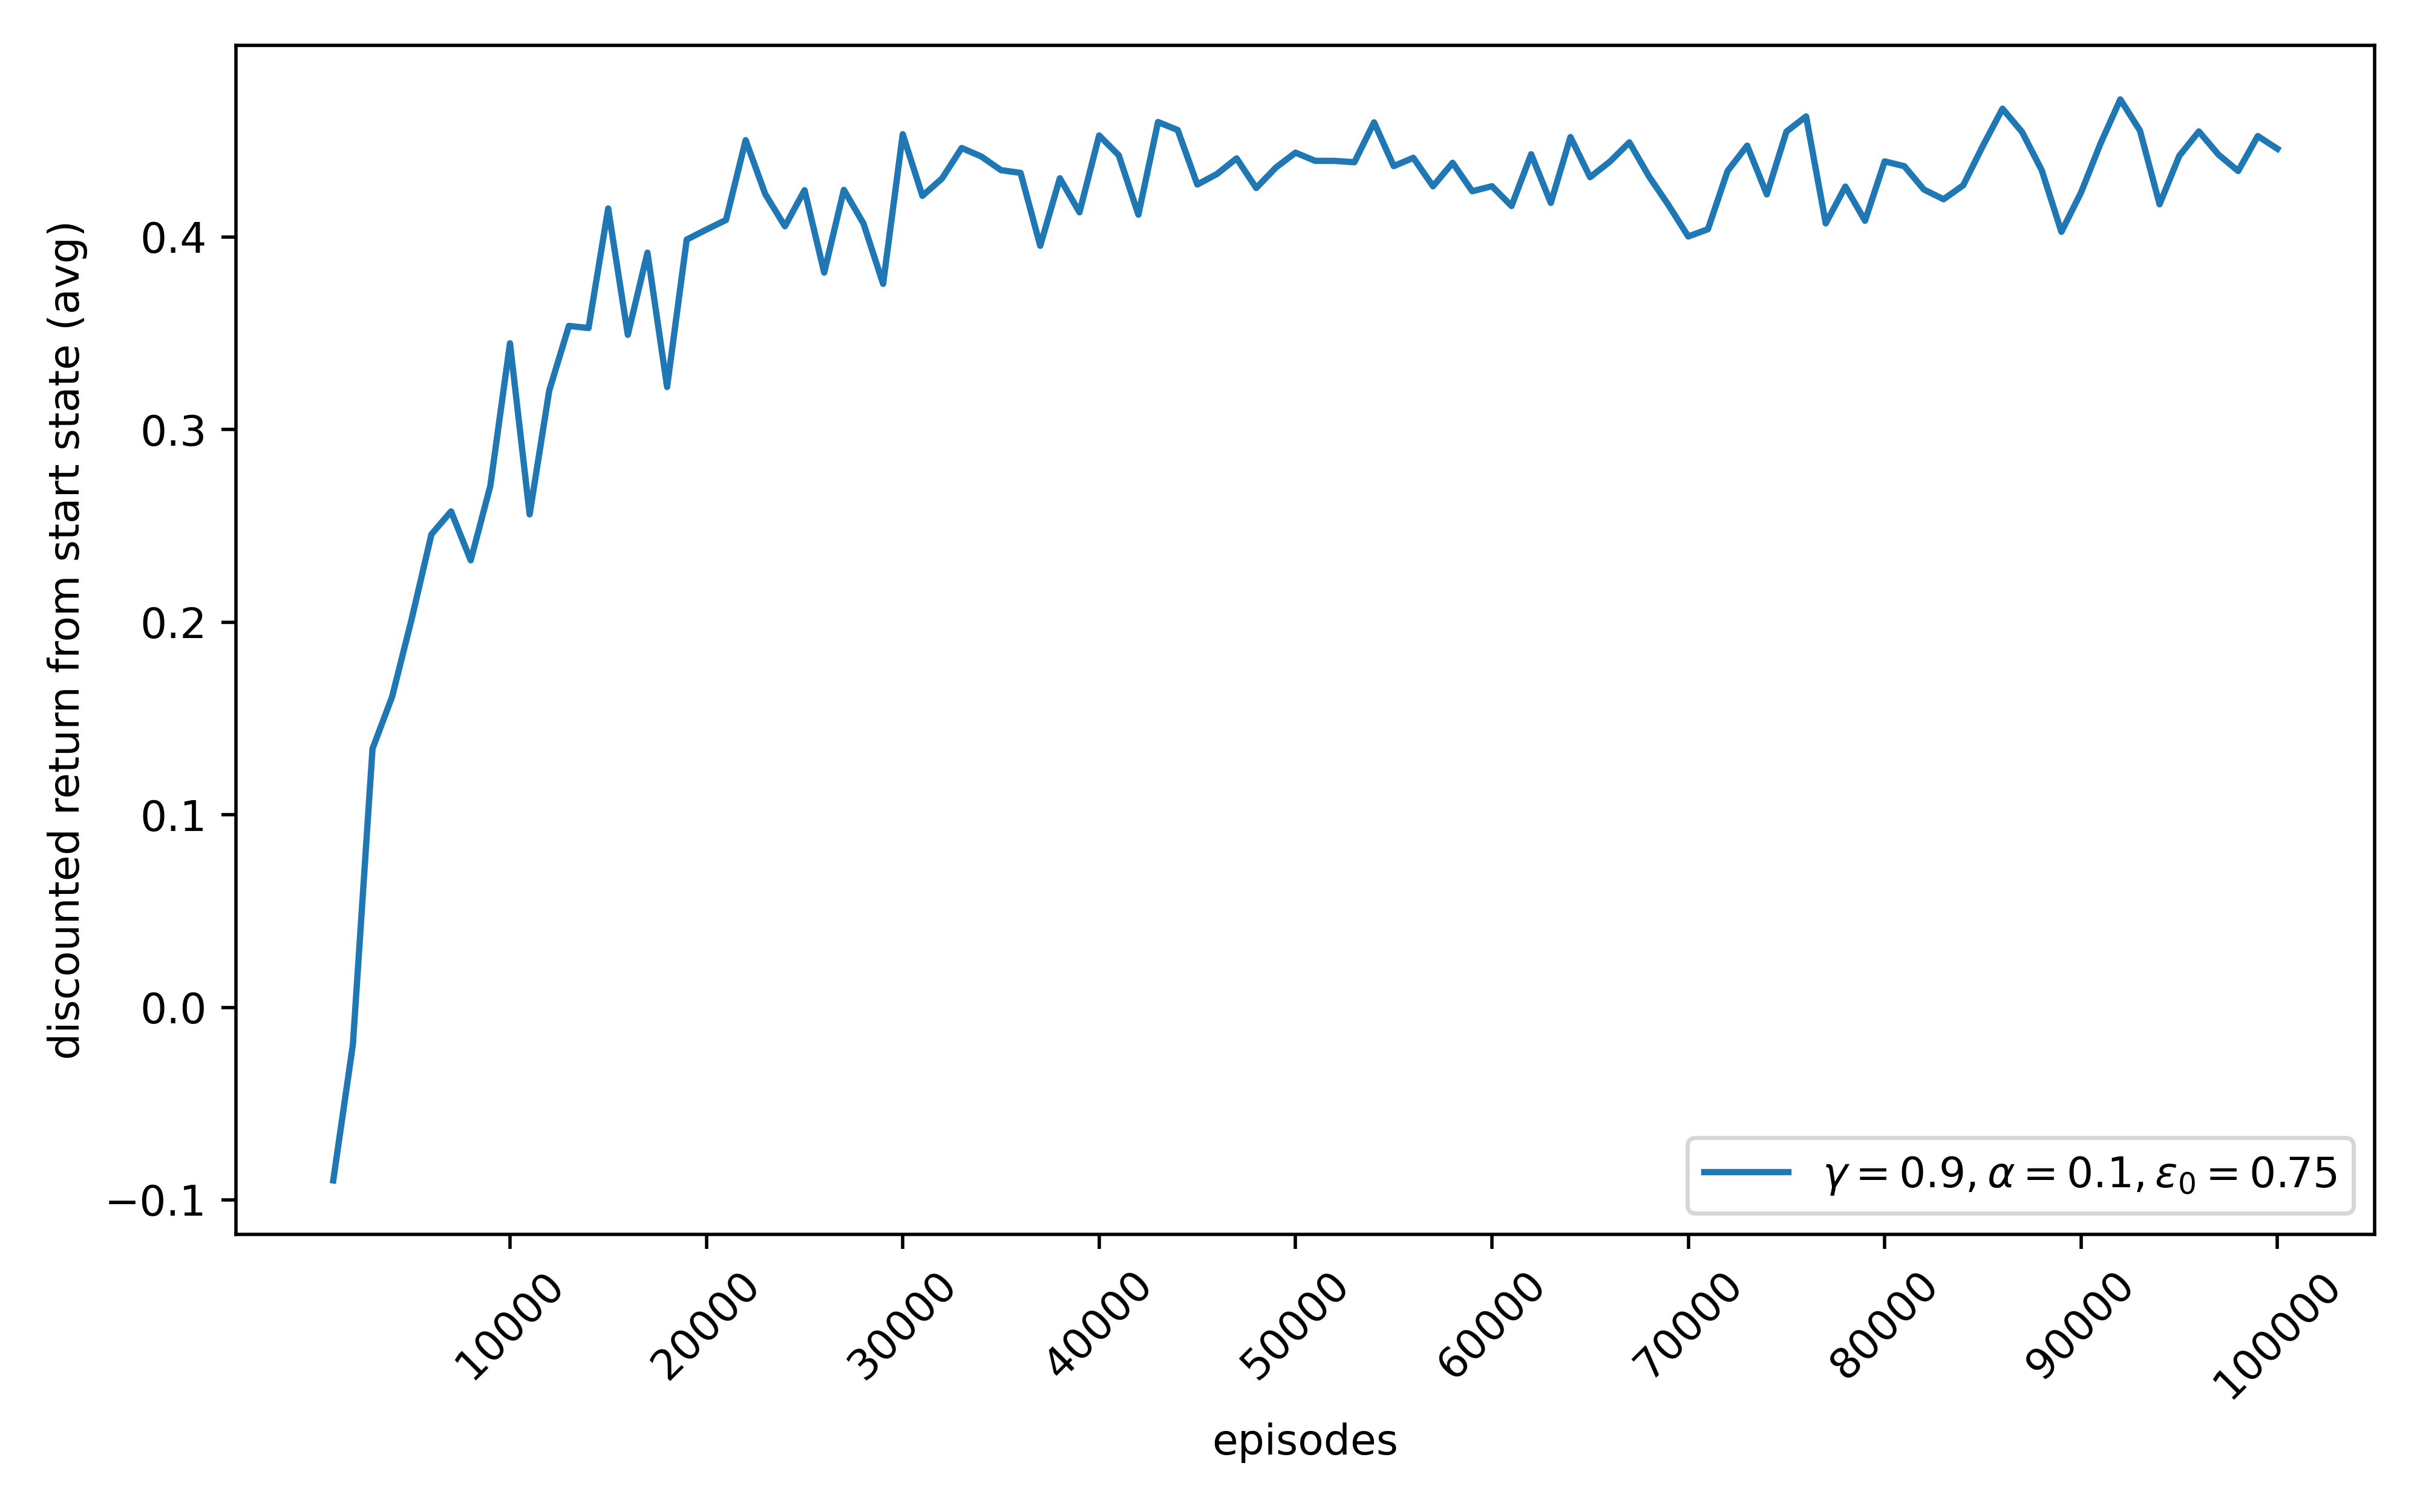
\includegraphics[width=\linewidth]{plots/part1-e.1-rewards.png}
        \caption{Discounted Return}
        
    \end{minipage}
    \hfill
    \begin{minipage}{0.49\linewidth}
        \centering
        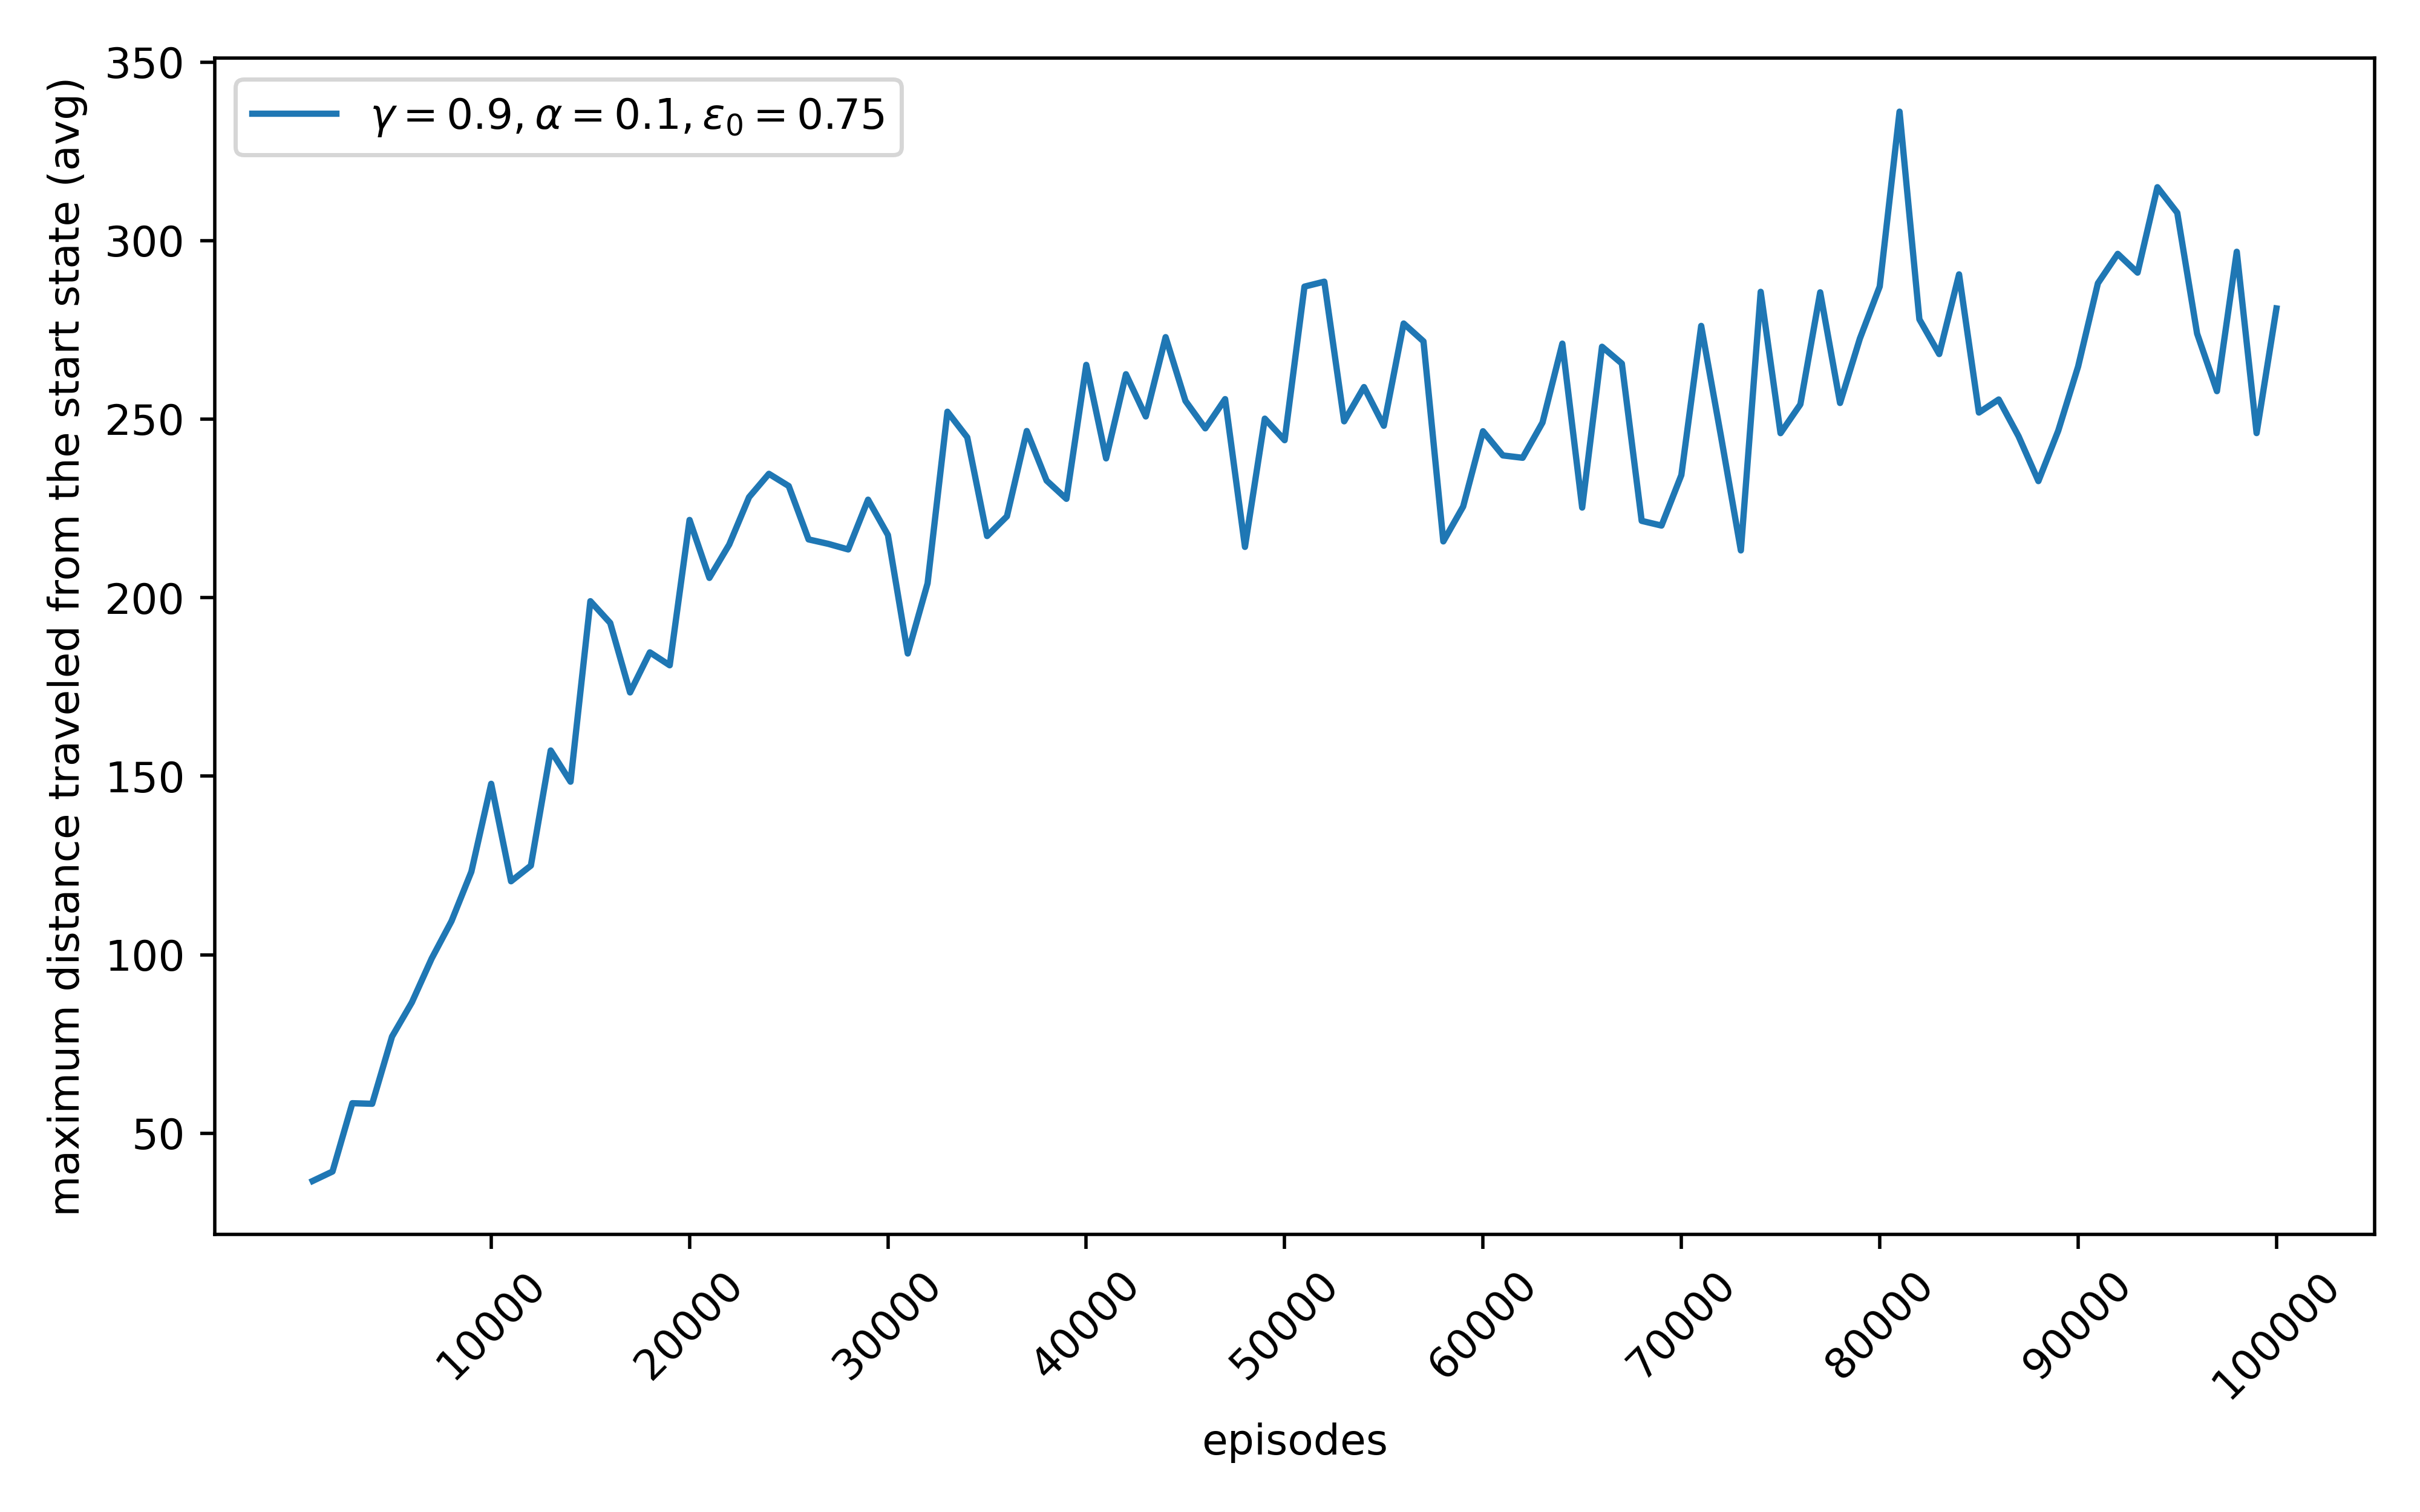
\includegraphics[width=\linewidth]{plots/part1-e.1-distances.png}
        \caption{Distance Traveled}
    \end{minipage}

    \vspace{1em}
    \begin{minipage}{\linewidth}
        \centering
        \begin{tabular}{lccc}
            \hline
            Episodes & Discounted Return & Average Distance \\
            \hline
            $98,000$ & $0.43$ & $296.87$ \\
            $99,000$ & $0.45$ & $246.07$ \\
            $100,000$ & $0.45$ & $280.99$ \\
            \hline
        \end{tabular}
        \caption{\texttt{Tabular} $\gamma = 0.9, \alpha = 0.1, \epsilon = 0.75$. Reward: \texttt{overtakes}.}
    \end{minipage}
     \label{fig:part1-e2}
\end{figure}

\begin{enumerate}
    \item From the \texttt{gifs} we observed that the agent drives faster (trying to overtake the other cars). This is in contrast to the case then reward is total distance traveled, where the agent tries to move in lanes that are empty and also reduces it's speed often in order to \textbf{remain far} from other car, to reduce chances of collisions with other cars.
\item Lane Visualization: See \autoref{fig:part1-e.1-lane-visualization}. We didn't see any clear difference from the total distance reward case. The agent prefers lanes where obstacles are farther away.
\item Speed Visualization:  See \autoref{fig:part1-e.1-speed-visualization}. The agent has a clear preference here for higher speeds, even when it is close to other cars, the agent doesn't assign higher value to slowing down, unlike when reward is total distance. 
\end{enumerate}

\begin{figure}[H]
    \centering
    \begin{minipage}{0.48\textwidth}
        \centering
        
\includegraphics[width=\linewidth]{plots/part1-e.1-lane_visualization_01_step_0420.png}
    \end{minipage}
    \hfill
    \begin{minipage}{0.48\textwidth}
        \centering
        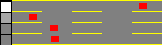
\includegraphics[width=\linewidth]{plots/part1-e.1-lane_visualization_00_step_1000.png}
    \end{minipage}
    \caption{Lane Visualization for Tabular Q-agent with \texttt{overtakes} reward}
    \label{fig:part1-e.1-lane-visualization}
\end{figure}

\begin{figure}[H]
    \centering
    \begin{minipage}{0.48\textwidth}
        \centering
        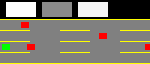
\includegraphics[width=\linewidth]{plots/part1-e.1-speed_visualization_02_step_0020.png}
    \end{minipage}
    \hfill
    \begin{minipage}{0.48\textwidth}
        \centering
        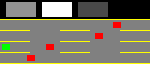
\includegraphics[width=\linewidth]{plots/part1-e.1-speed_visualization_00_step_0920.png}
    \end{minipage}
    \caption{Speed Visualization for Tabular Q-agent with \texttt{overtakes} reward}
    \label{fig:part1-e.1-speed-visualization}
\end{figure}




\subsection{Distance levels: $3$}

\begin{figure}[H]
    \centering
    \begin{minipage}{0.49\linewidth}
        \centering
        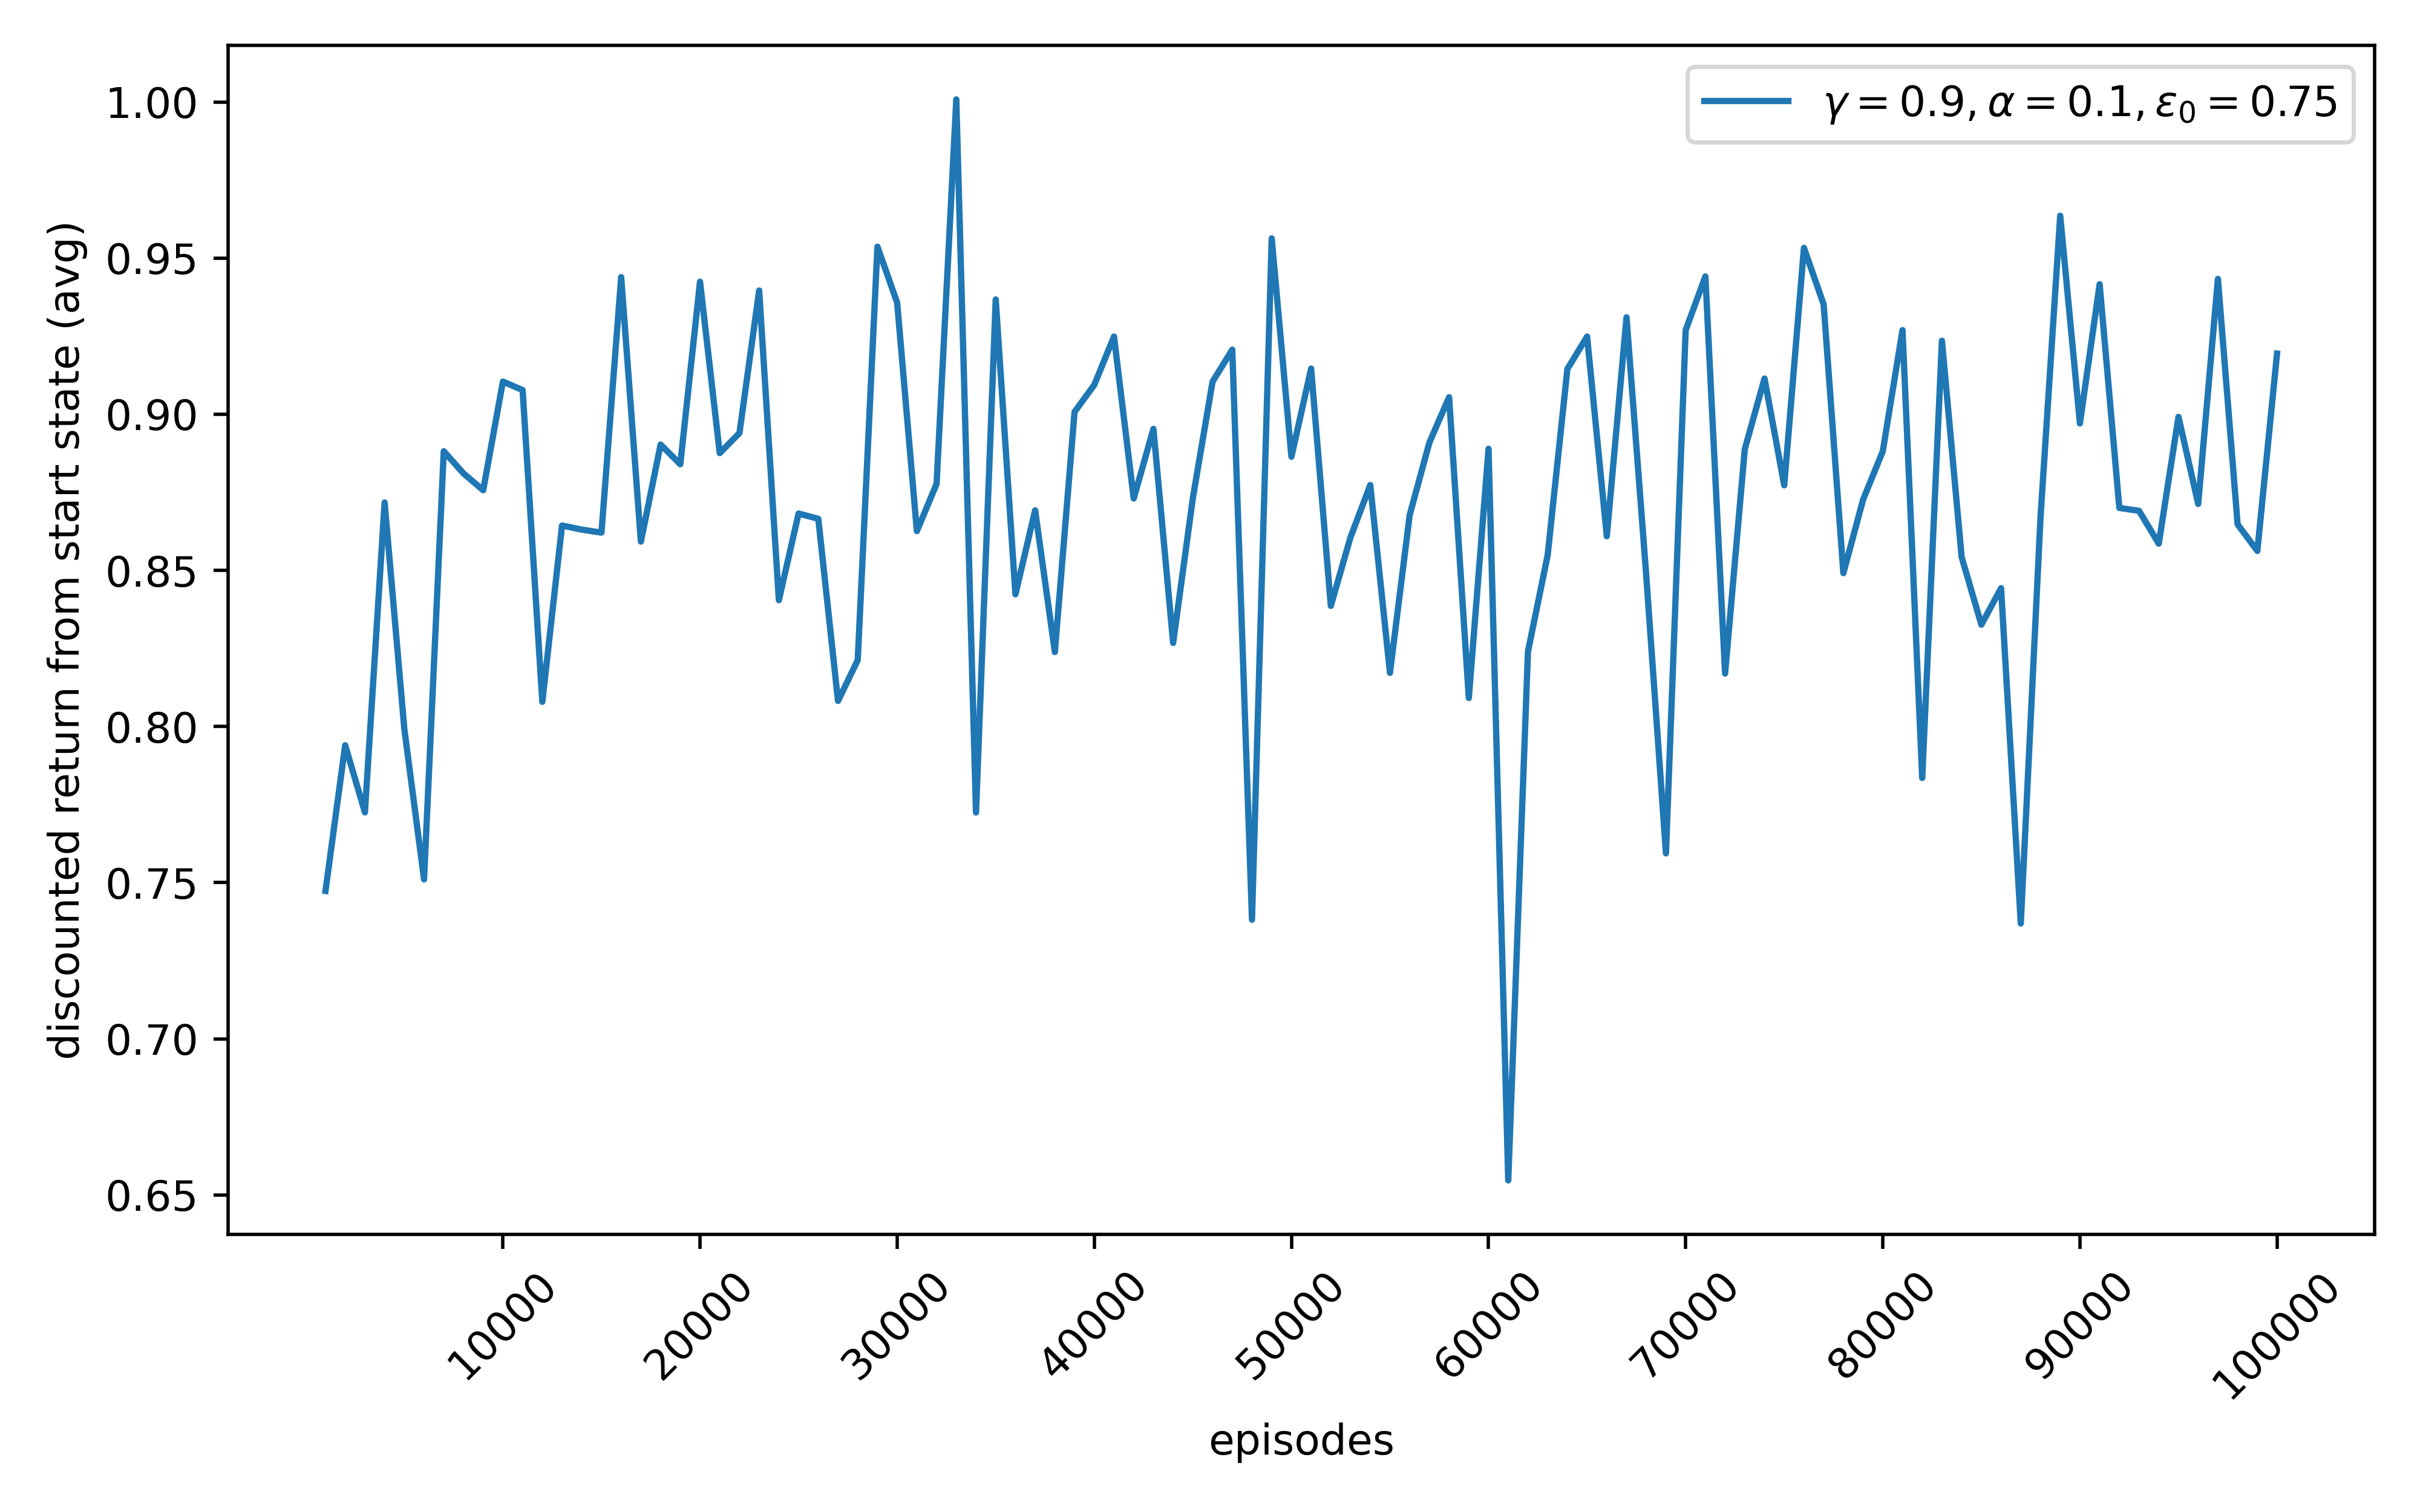
\includegraphics[width=\linewidth]{plots/part1-e.2-rewards.png}
        \caption{Discounted Return}
        
    \end{minipage}
    \hfill
    \begin{minipage}{0.49\linewidth}
        \centering
        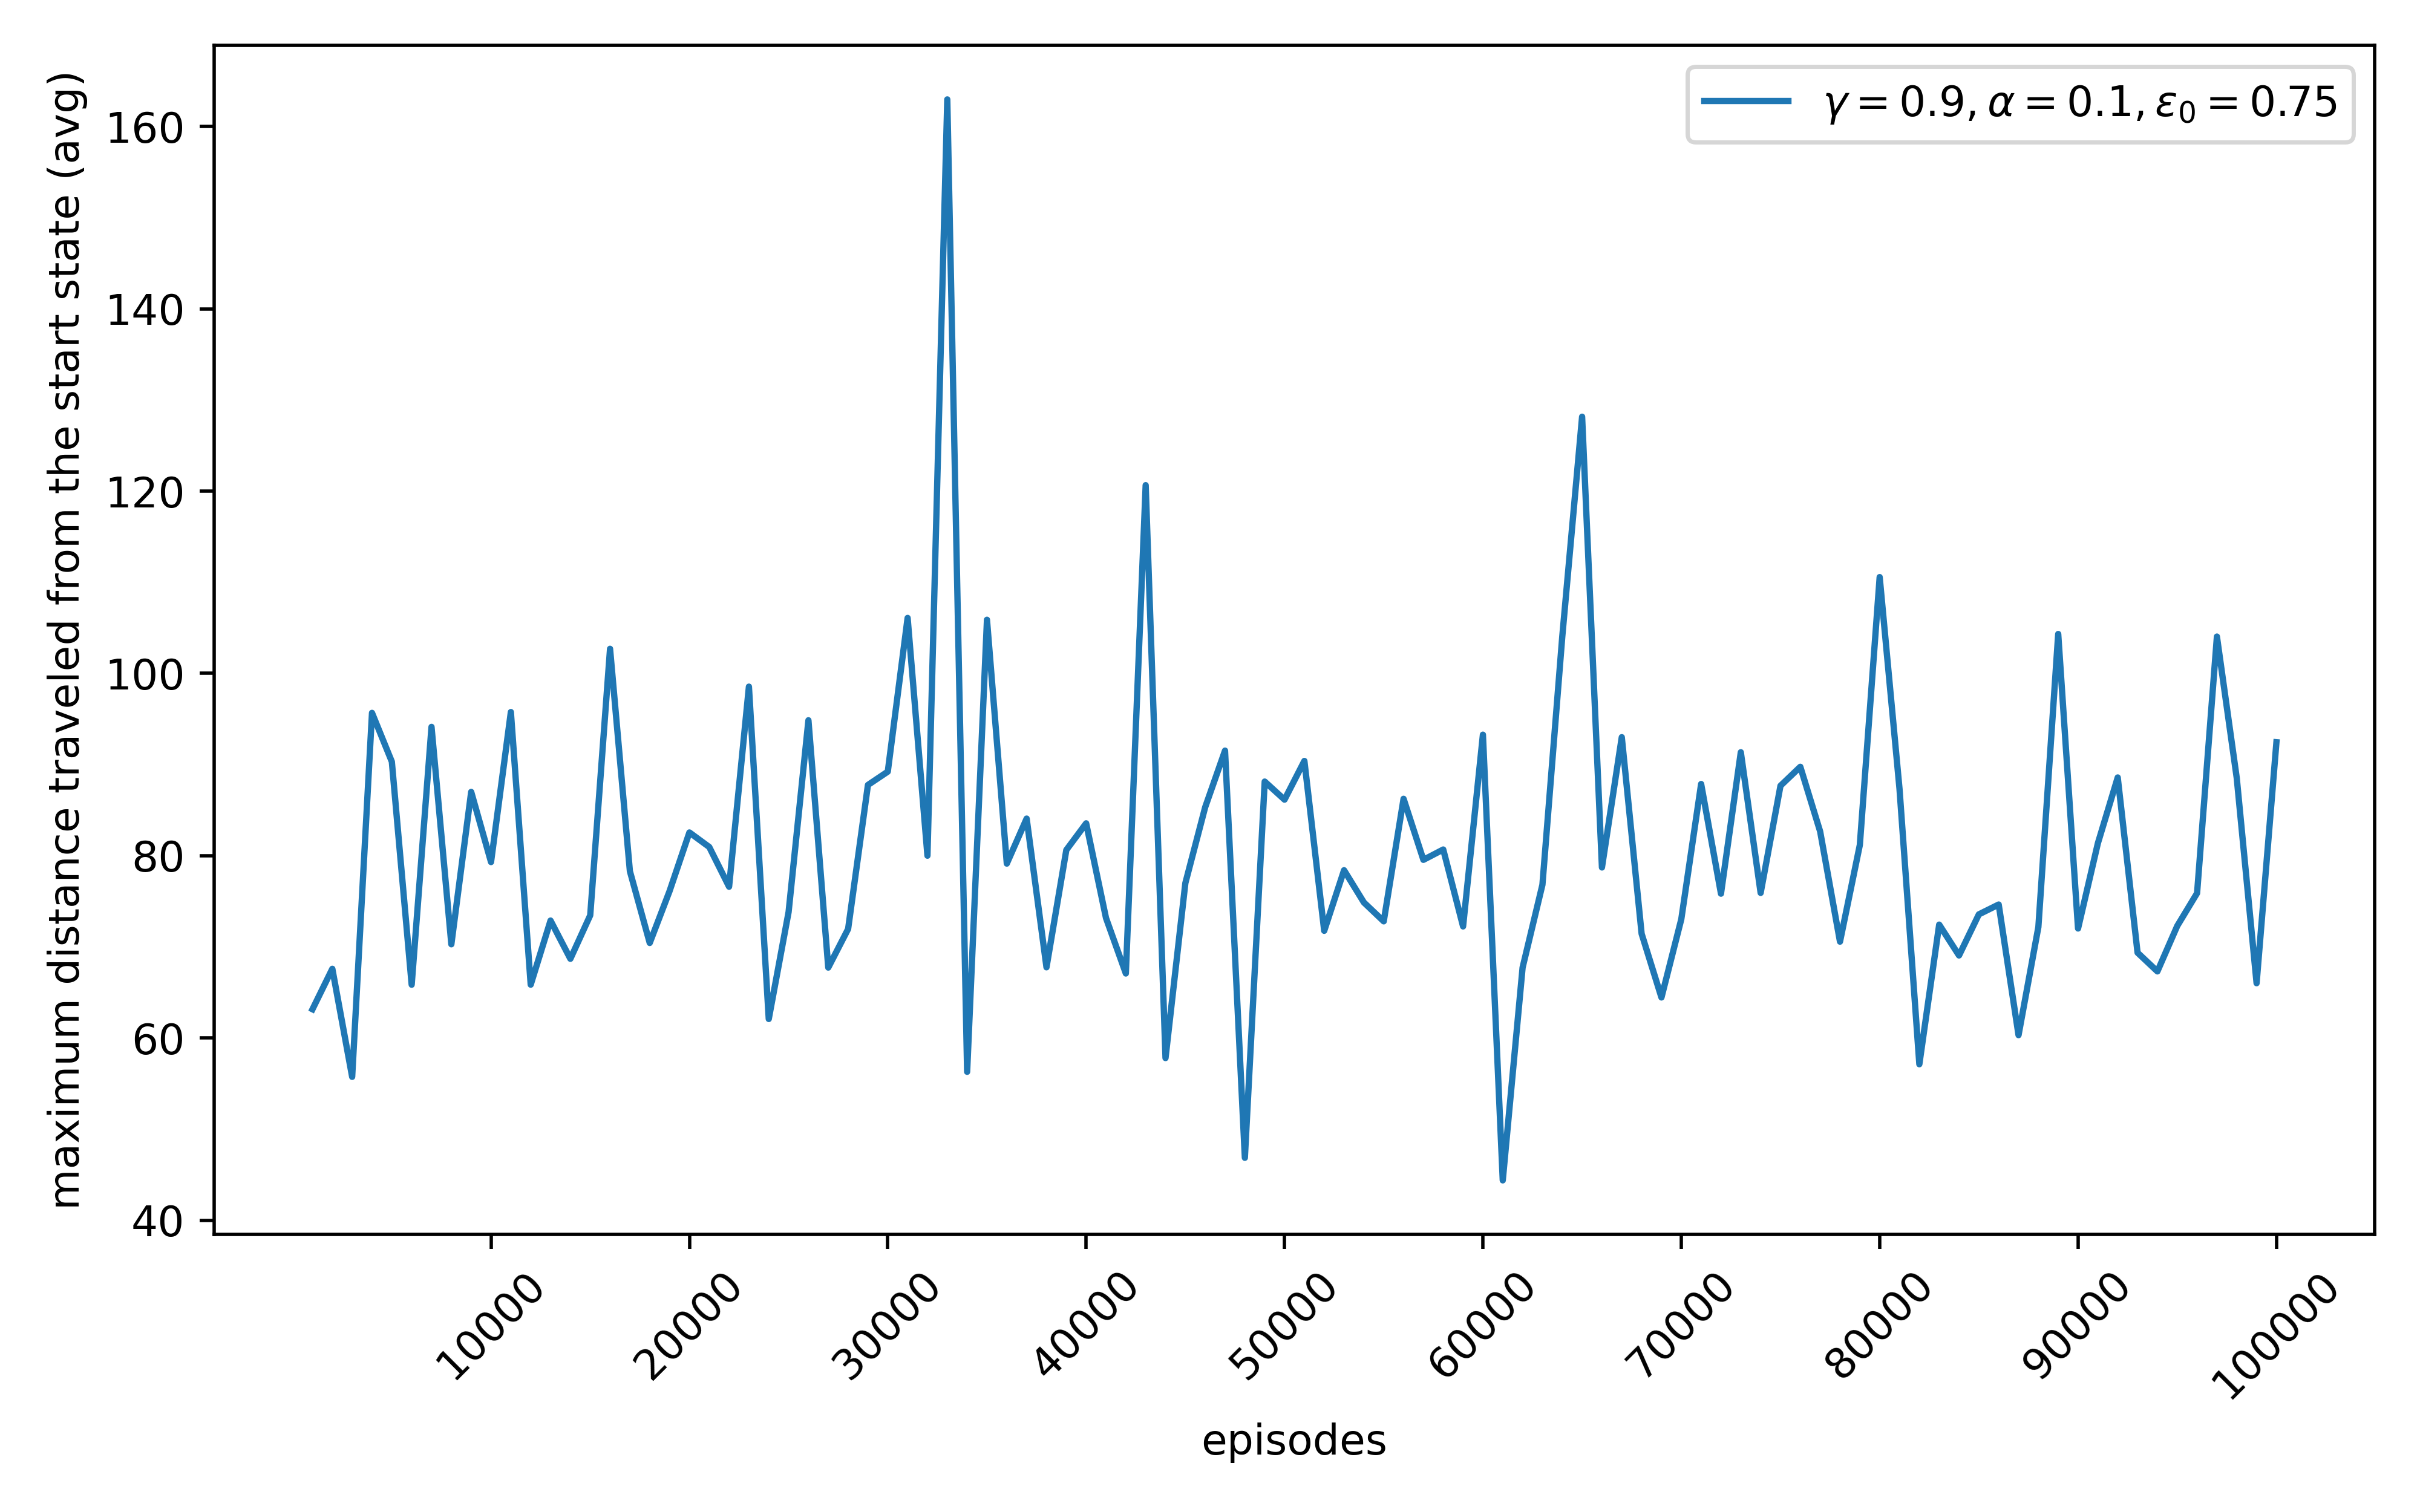
\includegraphics[width=\linewidth]{plots/part1-e.2-distances.png}
        \caption{Distance Traveled}
    \end{minipage}

    \vspace{1em}
    \begin{minipage}{\linewidth}
        \centering
        \begin{tabular}{lccc}
            \hline
            Episodes & Discounted Return & Average Distance \\
            \hline
            $98,000$ & $0.86$ & $88.52$ \\
            $99,000$ & $0.86$ & $66.02$ \\
            $100,000$ & $0.92$ & $92.46$ \\
            \hline
        \end{tabular}
        \caption{\texttt{Tabular} $\gamma = 0.9, \alpha = 0.1, \epsilon = 0.75$ and $3$ discrete levels of distance.}
    \end{minipage}
     \label{fig:part1-e2}
\end{figure}
\begin{enumerate}
\item We see that the total distance traveled is much less compared o the case of $5$ discrete levels. In the \texttt{gifs} we see that the agent starts "acting" (switching lanes) even when it is much far from the cars (compared to the $5$ levels case).

\item Lane Visualization: See \autoref{fig:part1-e.2-lane-visualization}. The agent is not able to differentiate well due to smaller level of discretization.
\item Speed Visualization:  See \autoref{fig:part1-e.2-speed-visualization}. Compared to \autoref{fig:part1-a-speed-visualization}, the difference is assigned value is lower for the similar settings. The obstacle has to come really close to the agent for it to notice.
\end{enumerate}

\begin{figure}[H]
    \centering
    \begin{minipage}{0.48\textwidth}
        \centering
        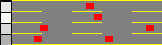
\includegraphics[width=\linewidth]{plots/part1-e.2-lane_visualization_00_step_0140.png}
    \end{minipage}
    \hfill
    \begin{minipage}{0.48\textwidth}
        \centering
        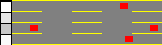
\includegraphics[width=\linewidth]{plots/part1-e.2-lane_visualization_00_step_0240.png}
    \end{minipage}
    \caption{Lane Visualization for Tabular Q-agent with $3$ levels of distance discretization}
    \label{fig:part1-e.2-lane-visualization}
\end{figure}

\begin{figure}[H]
    \centering
    \begin{minipage}{0.48\textwidth}
        \centering
        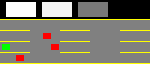
\includegraphics[width=\linewidth]{plots/part1-e.2-speed_visualization_00_step_0120.png}
    \end{minipage}
    \hfill
    \begin{minipage}{0.48\textwidth}
        \centering
        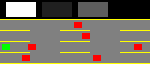
\includegraphics[width=\linewidth]{plots/part1-e.2-speed_visualization_00_step_0140.png}
    \end{minipage}
    \caption{Speed Visualization for Tabular Q-agent with $3$ levels of distance discretization}
    \label{fig:part1-e.2-speed-visualization}
\end{figure}

\section{Deep Q-Learning (Neural Network as Q-Function)}
\subsection{Architecture}\label{sec:arch}
\begin{enumerate}

\item For the Q-function, we use a Neural Network network with $2$ hidden layer of $32$ units each. The output layer has $5$ outputs , one corresponding to each action.
\item For the \texttt{discrete} case there are total 
$\texttt{n}_{\texttt{speed}} \times \texttt{n}_{\texttt{lanes}} \times  \texttt{n}_{\texttt{dist}}^{\texttt{n}_{\texttt{lanes}}} = 10,000$  states and we use embeddings of size $16$.
\item For the \texttt{discrete} case there are total 
$\texttt{n}_{\texttt{speed}} \times \texttt{n}_{\texttt{lanes}} = 16$ states and we use embeddings of size $4$. The distances $d_1, d_2, d_3, d_4$ are directly concatenated.
\end{enumerate}

\begin{figure}[H]
    \centering
    \begin{minipage}{0.49\linewidth}
        \centering
        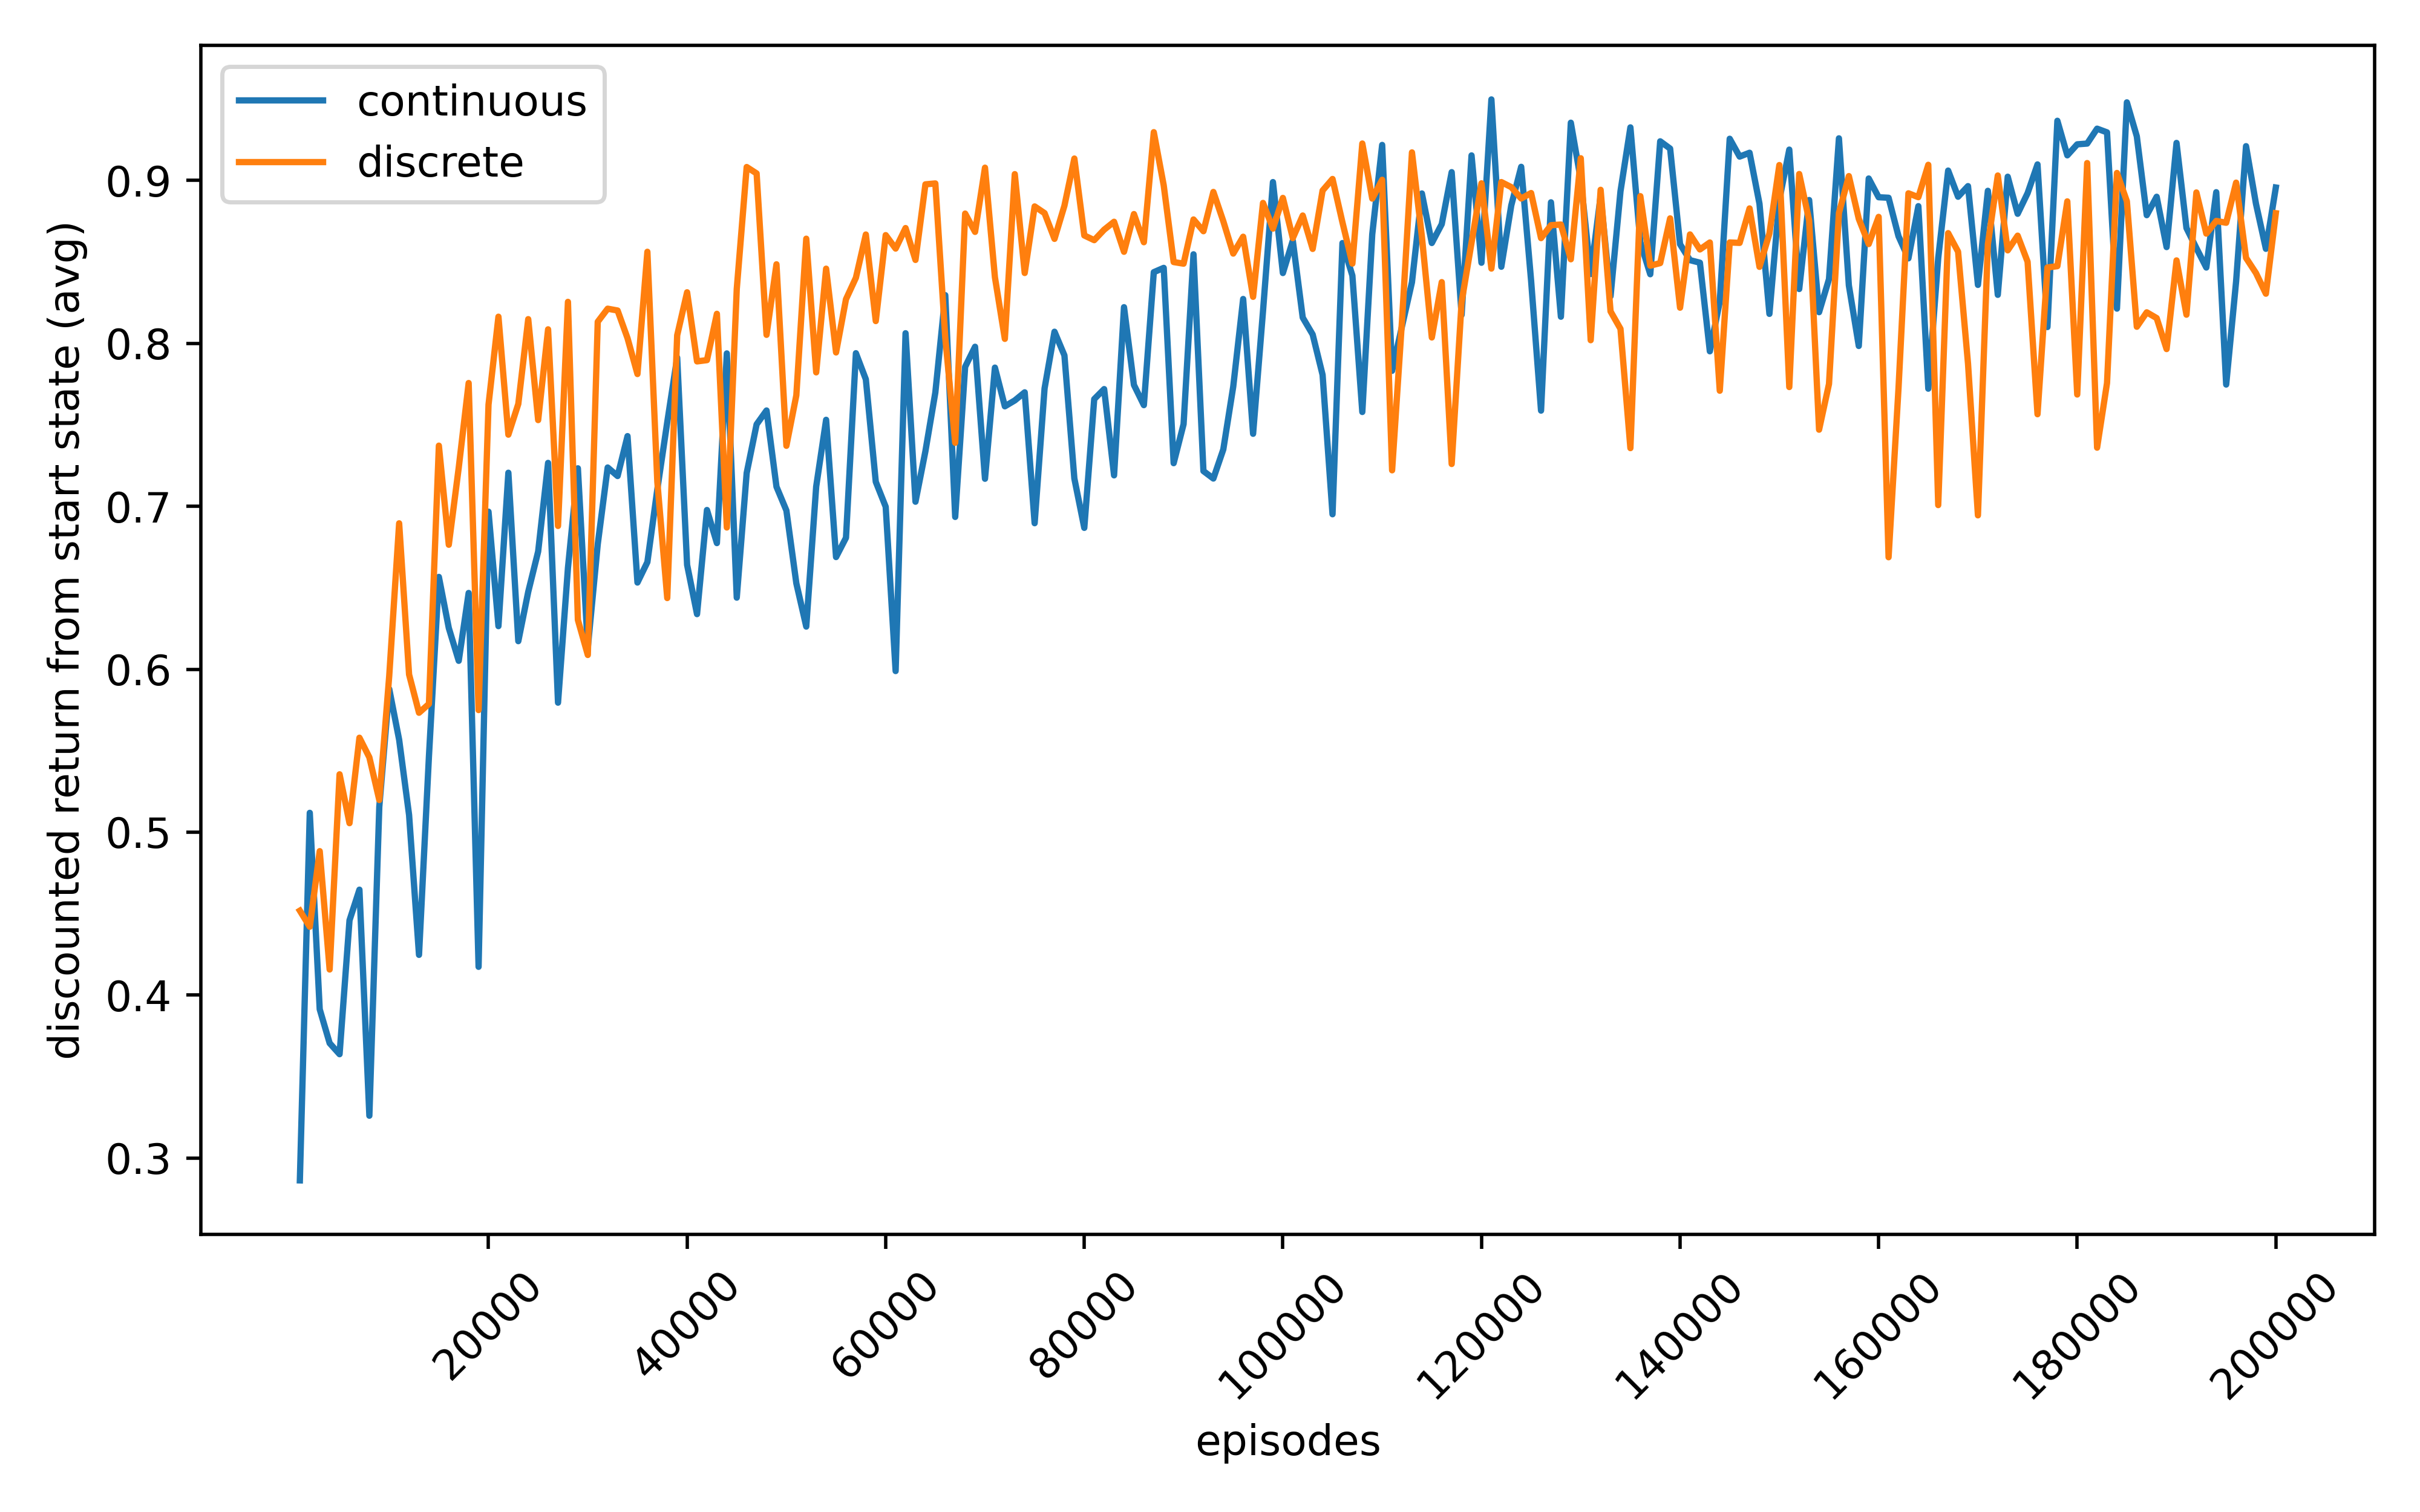
\includegraphics[width=\linewidth]{plots/part2-rewards.png}
        \caption{Discounted Return}
    \end{minipage}
    \hfill
    \begin{minipage}{0.49\linewidth}
        \centering
        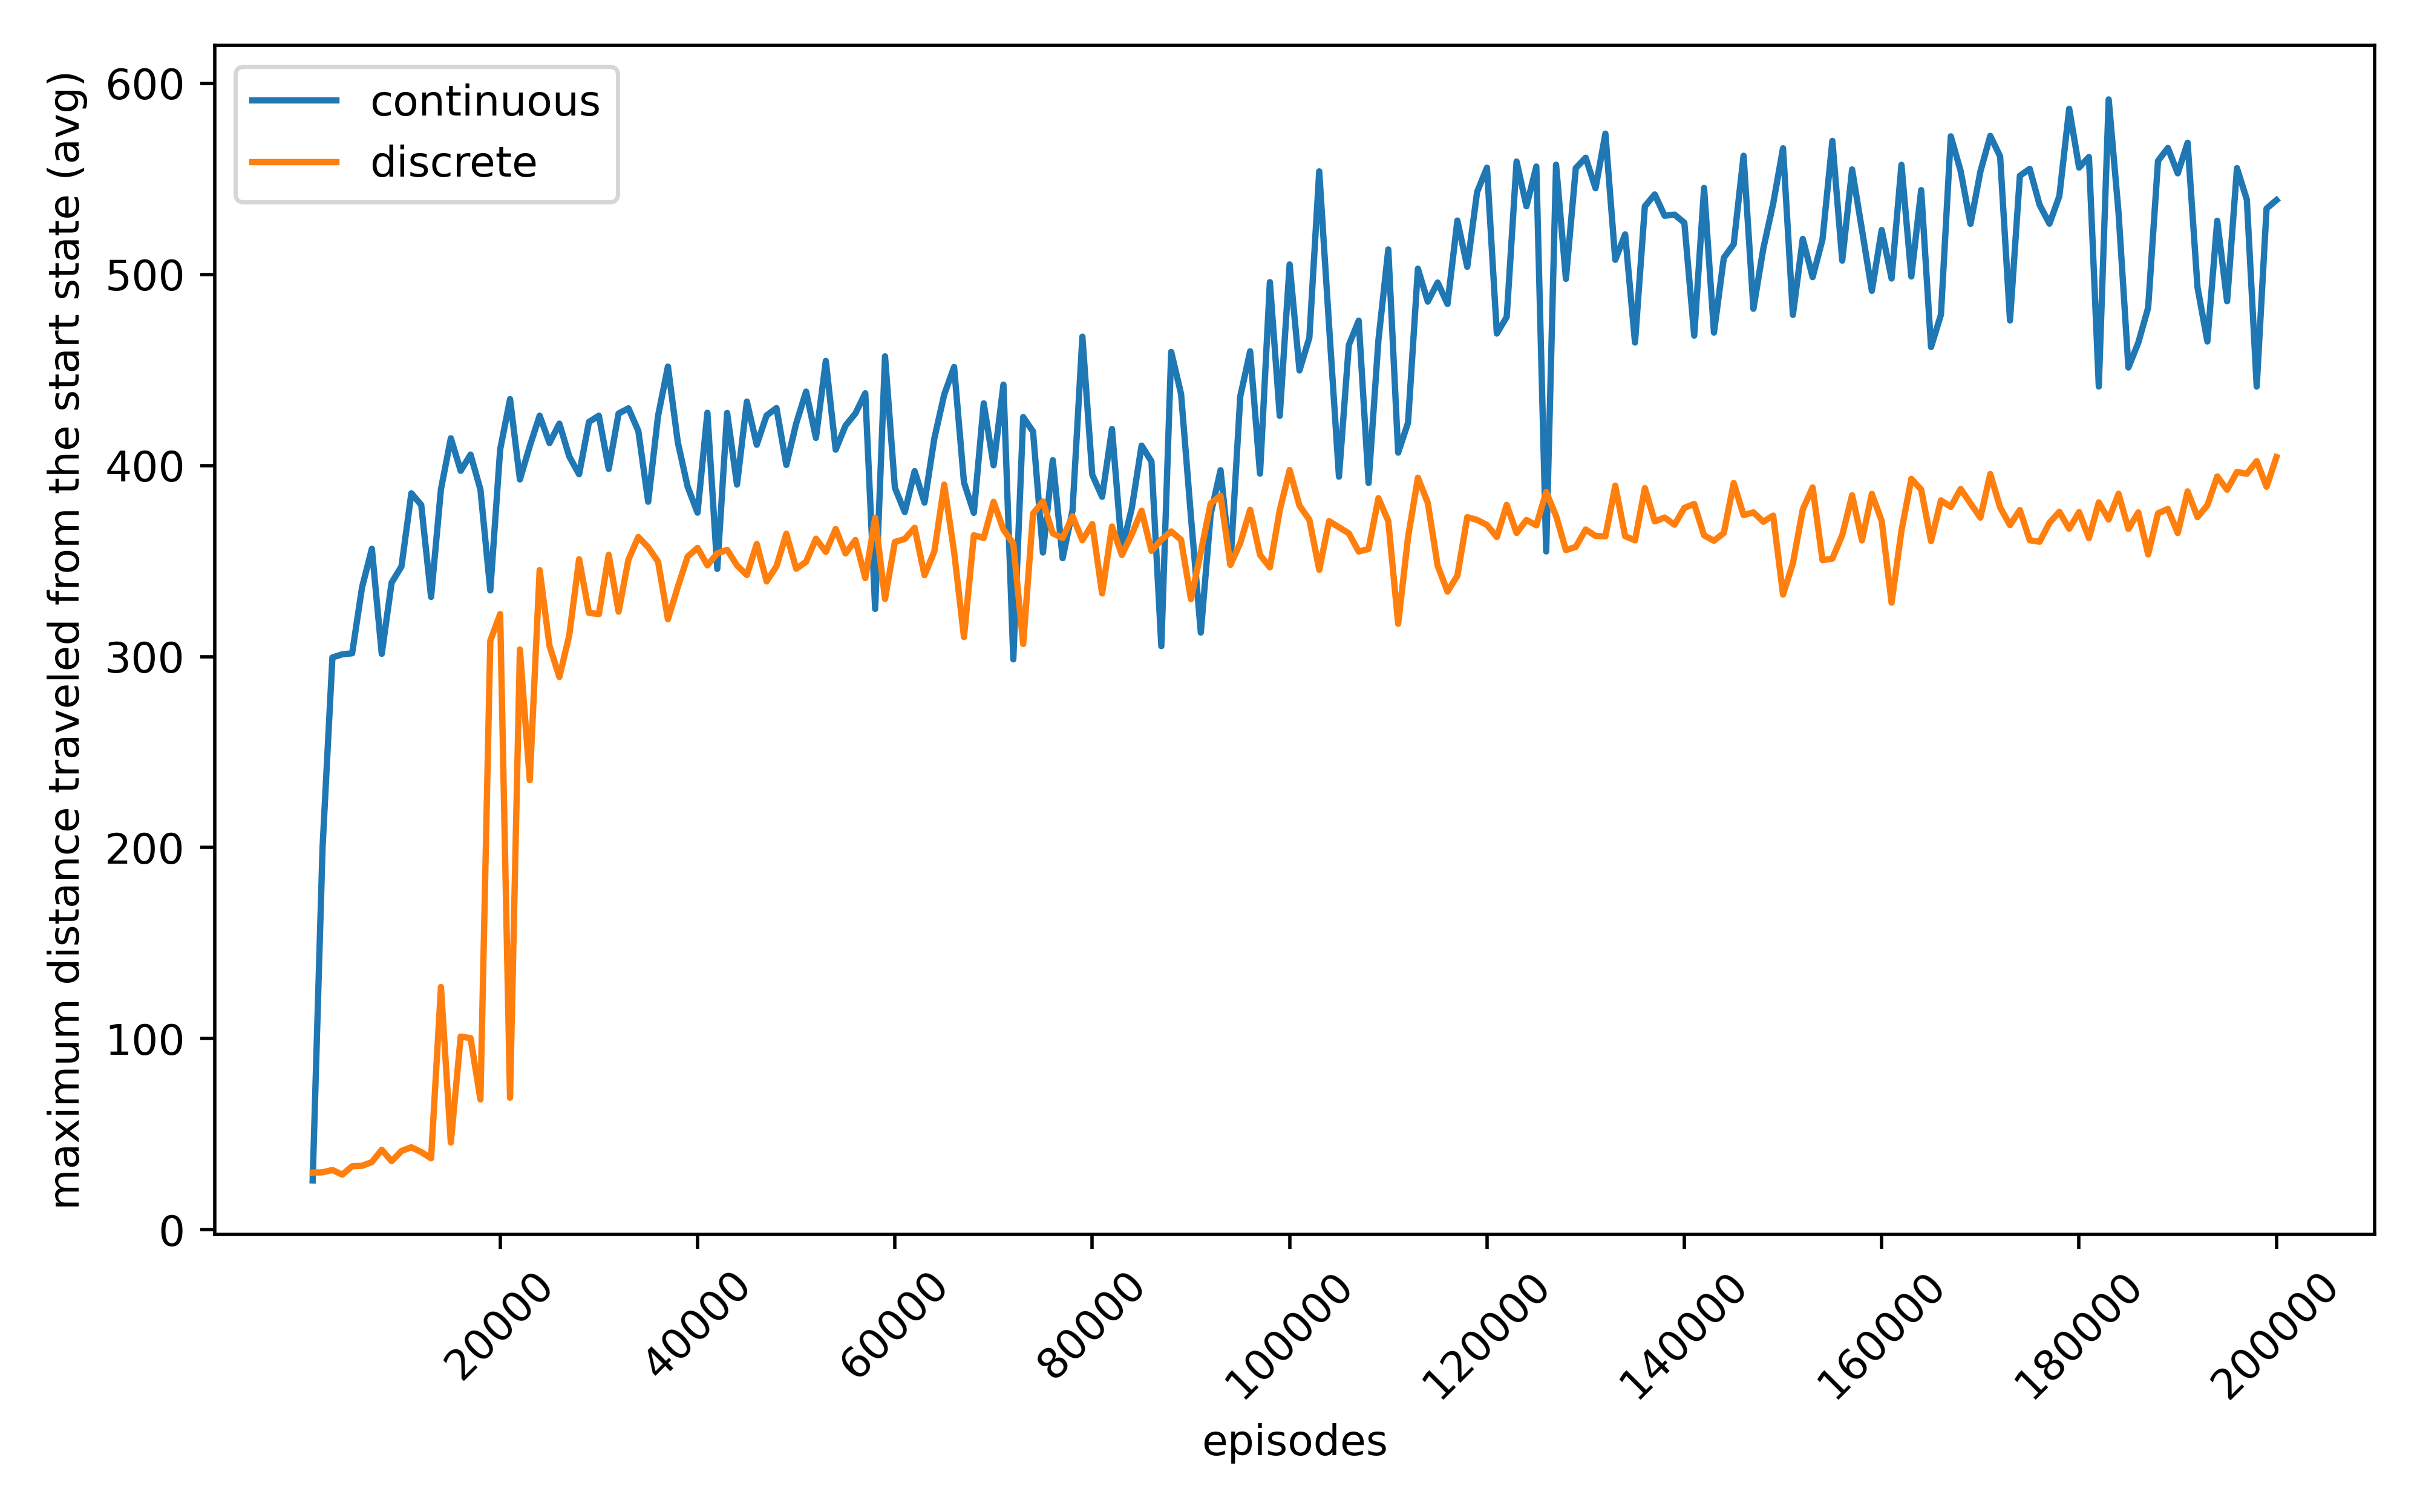
\includegraphics[width=\linewidth]{plots/part2-distances.png}
        \caption{Distance Traveled}
        \label{fig:part2-distance}
    \end{minipage}

    \vspace{1em}
    \begin{minipage}{\linewidth}
    \centering
    \begin{tabular}{lccc}
        \hline
        Model & Episodes & Discounted return & Average Distance \\
        \hline
        \texttt{Tabular} & $100,000$&$1.11$ & $531.98$ \\
        \texttt{DQN discrete}& $200,000$& $0.88$ & $404.42$ \\
        \texttt{DQN continuous} & $200,000$& $0.90$ & $538.91$ \\
        \hline
    \end{tabular}
    \caption{$\gamma = 0.9$, \texttt{Tabular} trained with $\alpha = 0.1, \epsilon = 0.75$,  \texttt{DQN} trained with \texttt{Adam} optimizer, learning rate = $10^{-4}$, batch size $256$ and replay buffer size $10,000$. For reference, maximum possible total discounted return is $1.2$.}
    \label{tab:part2}
    \end{minipage}
     \label{fig:part2}

\end{figure}
\texttt{DQN continuous} does better than \texttt{DQN discrete}. We believe this is because the $d_1, d_2, d_3, d_4$ are fed directly into the model. So the ordering, that for values of $d_1 = 0.2, 0.6, 0.9$ the order of closeness is implied. While in the discrete case, this has to be learned by the embedding layer. \texttt{DQN continuous} acts "identically" on $d_1  = 0.49$ or $d_1 = 0.51$.
\subsection{Visualization: \texttt{DQN Discrete}}
See \autoref{fig:part2.1-lane-visualization} and \autoref{fig:part2.1-speed-visualization}. The values assigned by the agent are absurd, also reflected in the low performance of the agent in \autoref{tab:part2}.


\begin{figure}[H]
    \centering
    \begin{minipage}{0.48\textwidth}
        \centering
        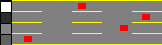
\includegraphics[width=\linewidth]{plots/part2.1-lane_visualization_00_step_0040.png}
    \end{minipage}
    \hfill
    \begin{minipage}{0.48\textwidth}
        \centering
        
\includegraphics[width=\linewidth]{plots/part2.1-lane_visualization_00_step_0200.png}
    \end{minipage}
    \caption{Lane Visualization for \texttt{DQN Discrete} agent}
    \label{fig:part2.1-lane-visualization}
\end{figure}

\begin{figure}[H]
    \centering
    \begin{minipage}{0.48\textwidth}
        \centering
        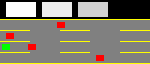
\includegraphics[width=\linewidth]{plots/part2.1-speed_visualization_00_step_0500.png}
    \end{minipage}
    \hfill
    \begin{minipage}{0.48\textwidth}
        \centering
        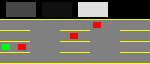
\includegraphics[width=\linewidth]{plots/part2.1-speed_visualization_00_step_0660.png}
    \end{minipage}
    \caption{Speed Visualization for    \texttt{DQN Discrete} agent}
    \label{fig:part2.1-speed-visualization}
\end{figure}


\subsection{Visualization: \texttt{DQN Continuous}}
See \autoref{fig:part2.2-lane-visualization} and \autoref{fig:part2.2-speed-visualization}. Preferences assigned are explainable, like in the Tabular-Q agent.


\begin{figure}[H]
    \centering
    \begin{minipage}{0.48\textwidth}
        \centering
        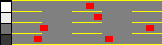
\includegraphics[width=\linewidth]{plots/part2.2-lane_visualization_00_step_0140.png}
    \end{minipage}
    \hfill
    \begin{minipage}{0.48\textwidth}
        \centering
        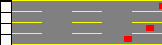
\includegraphics[width=\linewidth]{plots/part2.2-lane_visualization_00_step_0380.png}
    \end{minipage}
    \caption{Lane Visualization for \texttt{DQN Continuous} agent}
    \label{fig:part2.2-lane-visualization}
\end{figure}

\begin{figure}[H]
    \centering
    \begin{minipage}{0.48\textwidth}
        \centering
        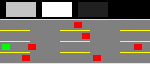
\includegraphics[width=\linewidth]{plots/part2.2-speed_visualization_00_step_0140.png}
    \end{minipage}
    \hfill
    \begin{minipage}{0.48\textwidth}
        \centering
        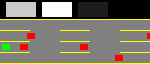
\includegraphics[width=\linewidth]{plots/part2.2-speed_visualization_01_step_0880.png}
    \end{minipage}
    \caption{Speed Visualization for    
    \texttt{DQN Continuous} agent}
    \label{fig:part2.2-speed-visualization}
\end{figure}



\section{Experimenting and Improving the Agent}
\subsection{Reward-Goal Relationship}\label{sec:reward-goal}
Out goal is to maximize the total distance traveled by the agent. The total discounted return (that the agent tries to maximize) is a proxy for the goal.

\begin{equation}\label{eqn:reward_vanilla}
r(state_t, a_t, state_{t+1}) = \begin{cases}
-5 & \texttt{if control car collides } \\
0.03*s_{t+1} & \texttt{otherwise}
 \end{cases} 
\end{equation}
\begin{align*}
\texttt{Distance} &= \Delta t (s_1 + s_2 + s_3 \dots)\\
\texttt{Discounted Return} &= 0.03 (s_1 + \gamma s_2 + \gamma^ 2 s_3 \dots)
\end{align*}

\begin{enumerate}
    \item While training, we see that sometimes the total discounted return earned increases while total distance traveled decreases. This might happen because the car prioritizes higher speeds earlier and that may lead to a crash. 

    \item As we increases $\gamma \to 1$, the total discounted return is more aligned with the total distance but training becomes unstable, often also reducing performance.
\end{enumerate}

\begin{figure}[H]
    \centering
    \begin{minipage}{0.49\linewidth}
        \centering
        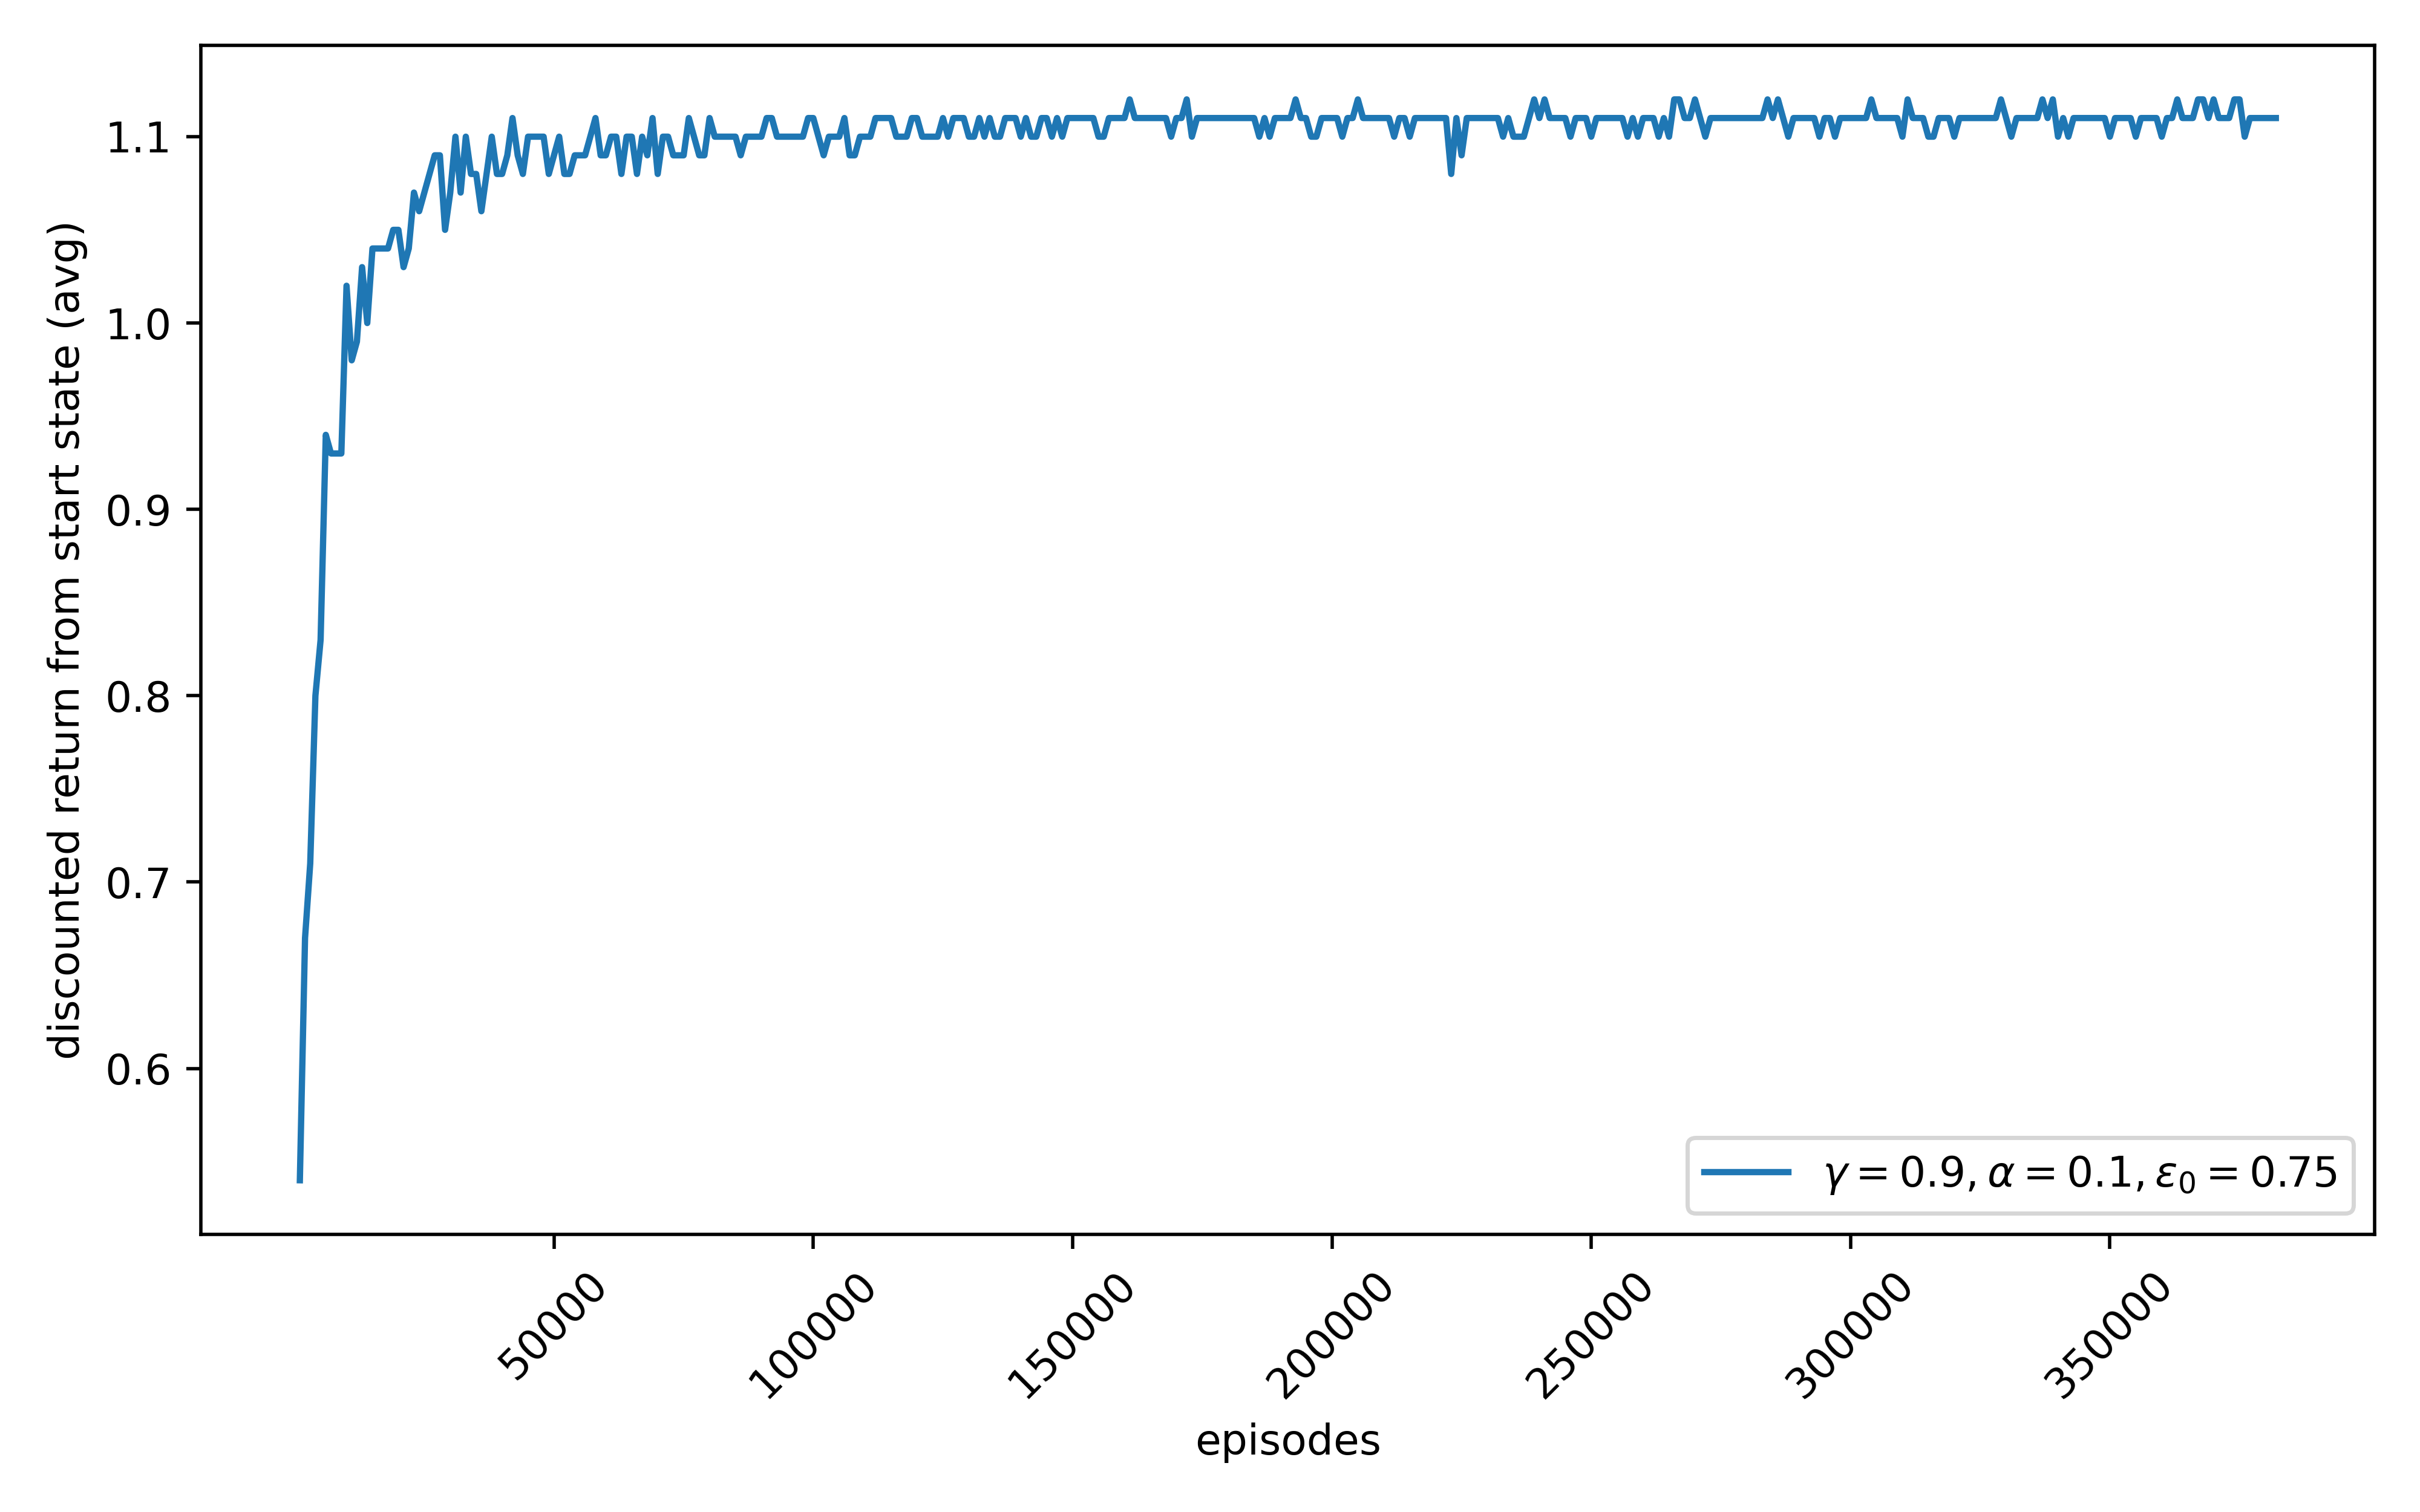
\includegraphics[width=\linewidth]{plots/part3-tabular-bad-rewards.png}
        \caption{Discounted Return}
    \end{minipage}
    \hfill
    \begin{minipage}{0.49\linewidth}
        \centering
        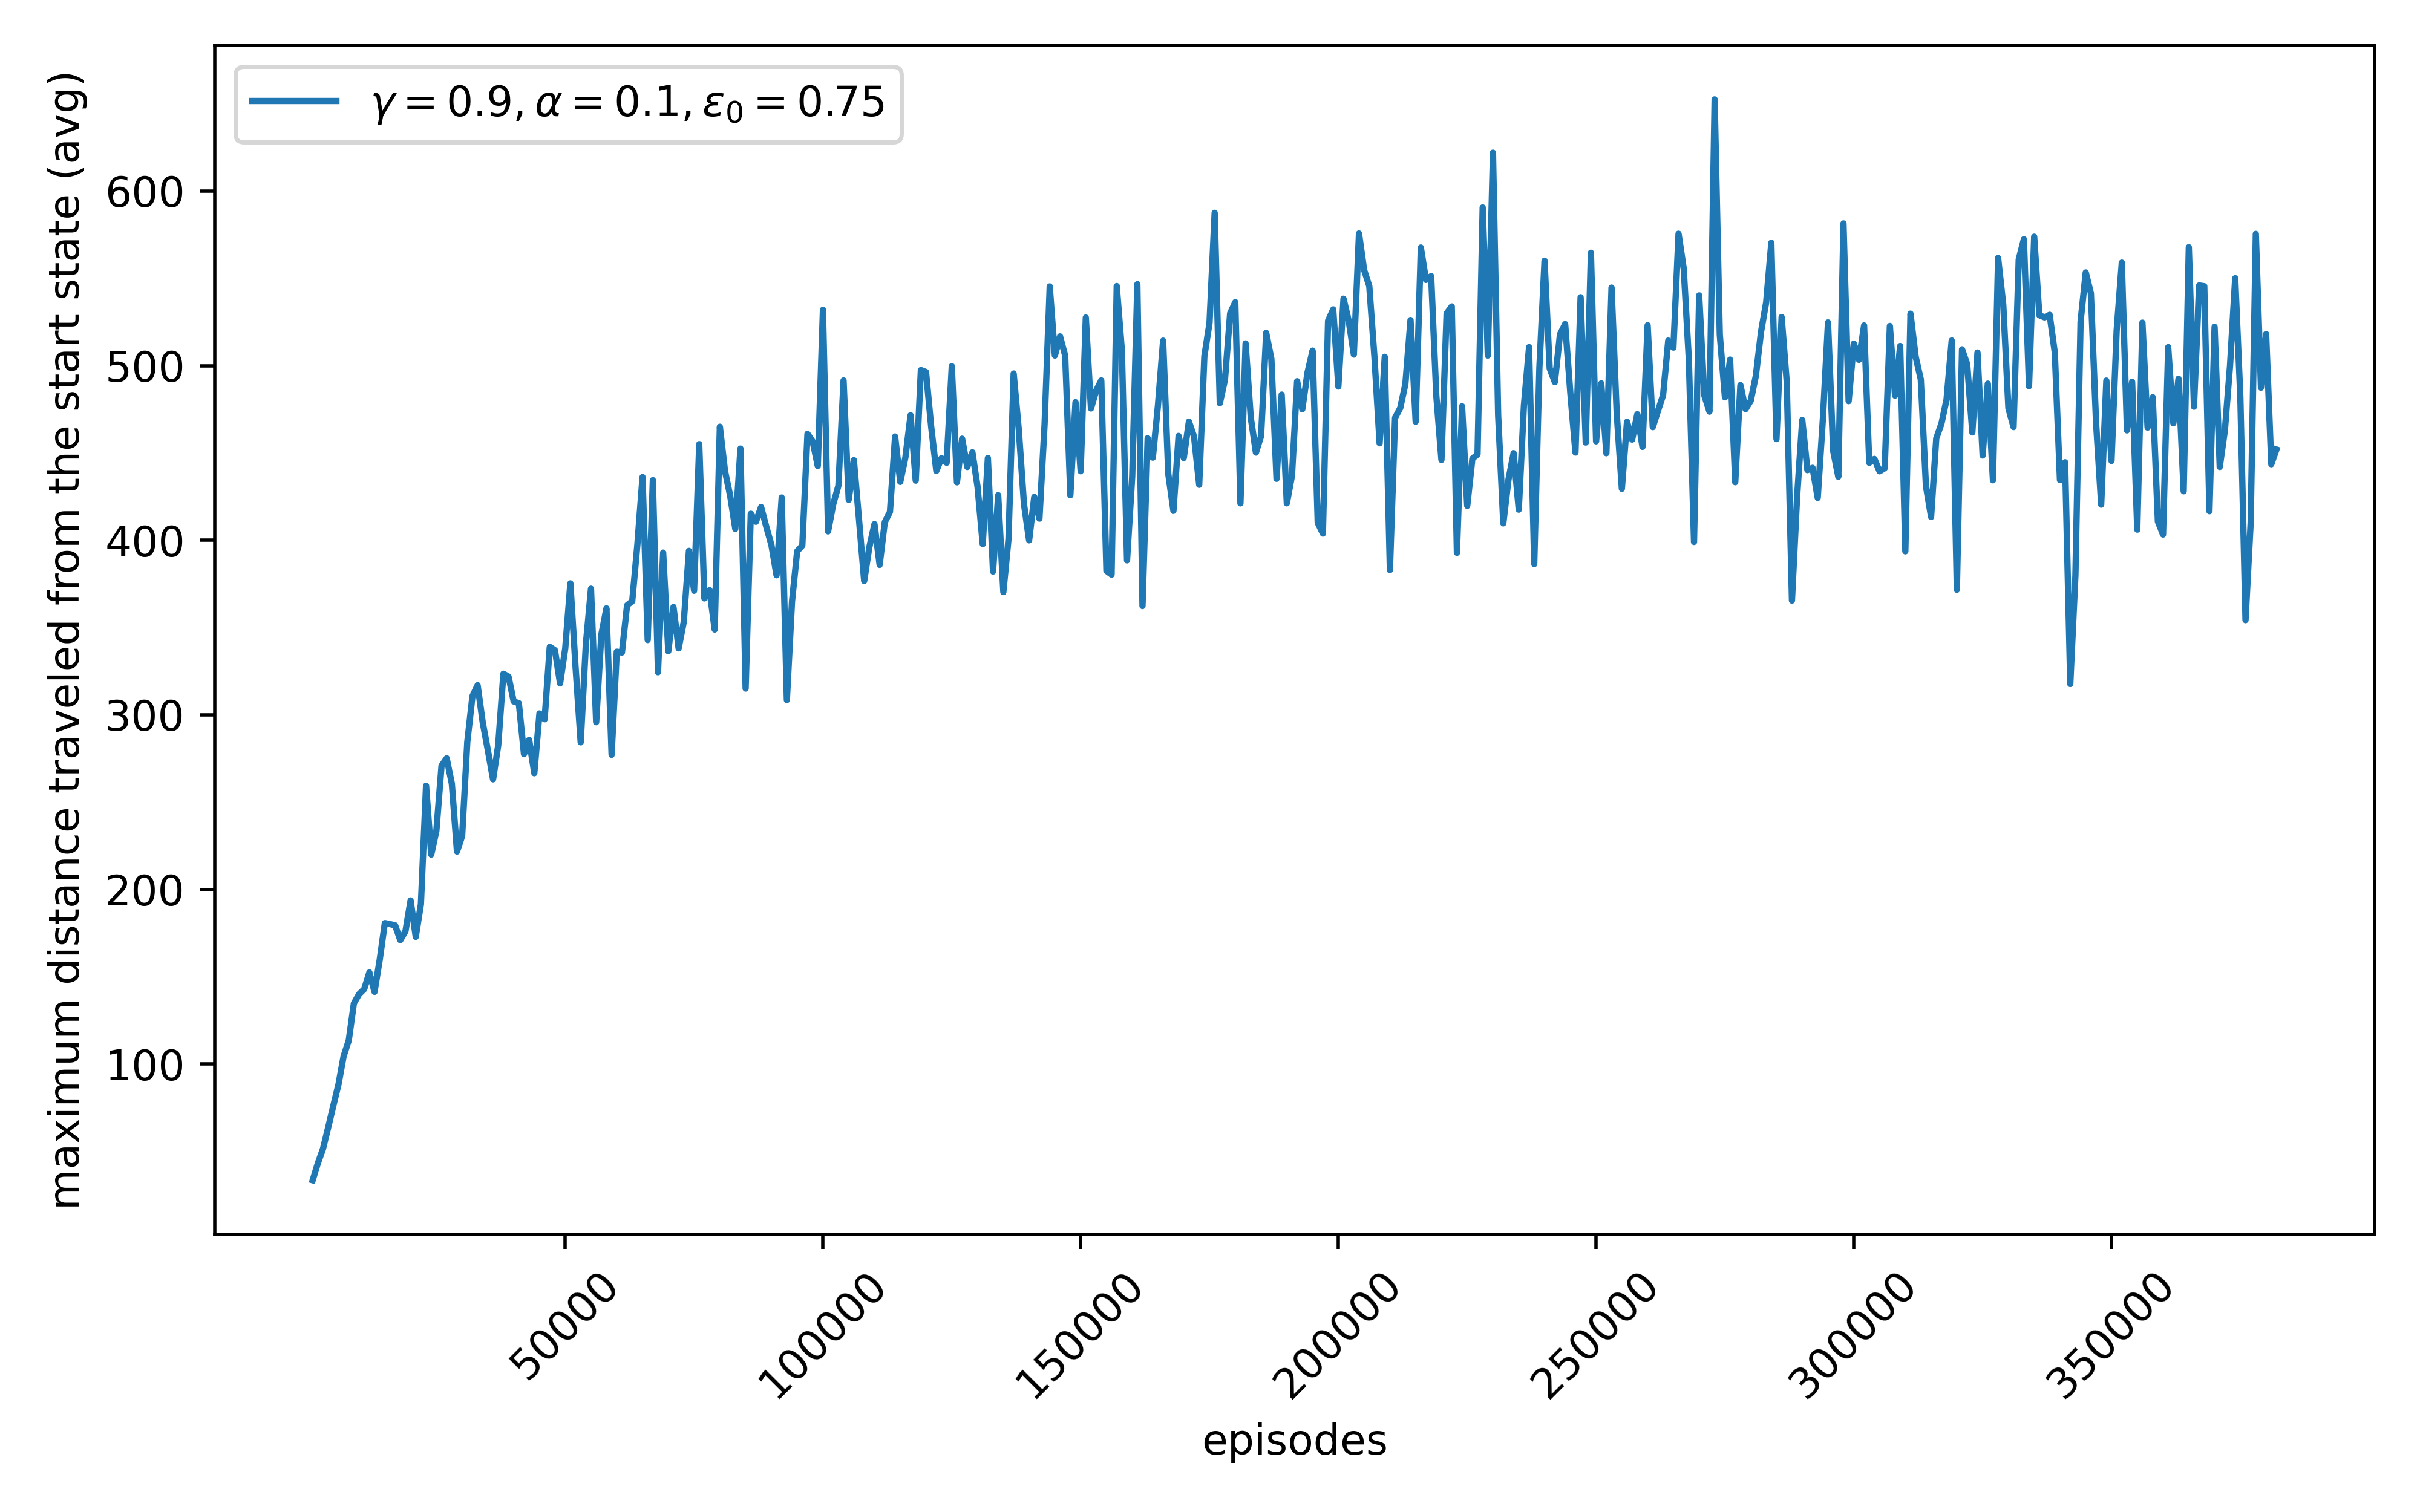
\includegraphics[width=\linewidth]{plots/part3-tabular-bad-distances.png}
        \caption{Distance Traveled}
    \end{minipage}
    \caption{\texttt{Tabular} $\gamma = 0.9, \alpha = 0.1, \epsilon = 0.75$. Further training after $100,000$ iterations does not improve performance.}
    \label{fig:part3-tabular}
\end{figure}

\subsection{Double DQN}
Here, a separate network is used for computing \texttt{target}. This network is updated "slowly". This approach aims to stabilize training. In vanilla DQN, the \texttt{prediction} and \texttt{target} networks both keep moving. 
\begin{align*}
    \texttt{target} &\gets r + \gamma \max_{a'} Q_{target}(s_{t + 1}, a')\\
    \texttt{prediction} &\gets Q_{policy}(s_t, a_t)
\end{align*}
$Q_{policy}$ is trained using gradients. $Q_{target}$ is updated as
\begin{align*}
    \theta_{target} \gets (1 - \tau)  \theta_{target} + \tau \theta_{policy}
\end{align*}
\subsection{Experiments: Optimizers}
\begin{enumerate}
    \item We experimented with \texttt{Adam} and \texttt{AdamW} optimizers with various variations of \texttt{amsgrad}, \texttt{weight\_decay} and $\gamma$ intending that more stable training would allow increasing $\gamma$. The NN architecture used was same as in \nameref{sec:arch}.
    \item We also trained with batch size $512$ but it didn't help. We then moved to a deeper network for the Q-function, described in \nameref{sec:ddqn} leading to the \texttt{DDQN-Vanilla} model.

    \item While training \texttt{DDQN-Vanilla} and \texttt{DDQN-Time-Embed} we also clip gradients to $100$.


\end{enumerate}
\subsection{Designing Reward}\label{sec:reward_design}
\begin{enumerate}
    \item Results in \autoref{tab:part1-d-linear} suggest that linearly decreasing $\epsilon$ works much better than other strategies. In the \texttt{DDQN} case we saw however that the distance traveled down starts going down later. We set a minimum on the $\epsilon$.

    \item To penalize earlier crashes more, we set the reward for crash to
    \begin{equation*}
       \texttt{reward}_{\texttt{crash}} =  -5\left(1 - \frac{\texttt{num\_steps}}{\texttt{episode\_max\_length}}
       \right)
    \end{equation*}
    \item To favor longer runs we add an increasing living reward
        \begin{equation*}
       \texttt{reward}_{\texttt{living}} =  0.15 \frac{\texttt{num\_steps}}{\texttt{episode\_max\_length}}
    \end{equation*}
    \item For the above reward to work, we also add the current timestep as $\left(\frac{\texttt{num\_steps}}{\texttt{episode\_max\_length}}\right)$ to the state. 
\end{enumerate}


\begin{figure}[H]
    \centering
    % First Row - Plots
    \begin{minipage}{0.32\linewidth}
        \centering
        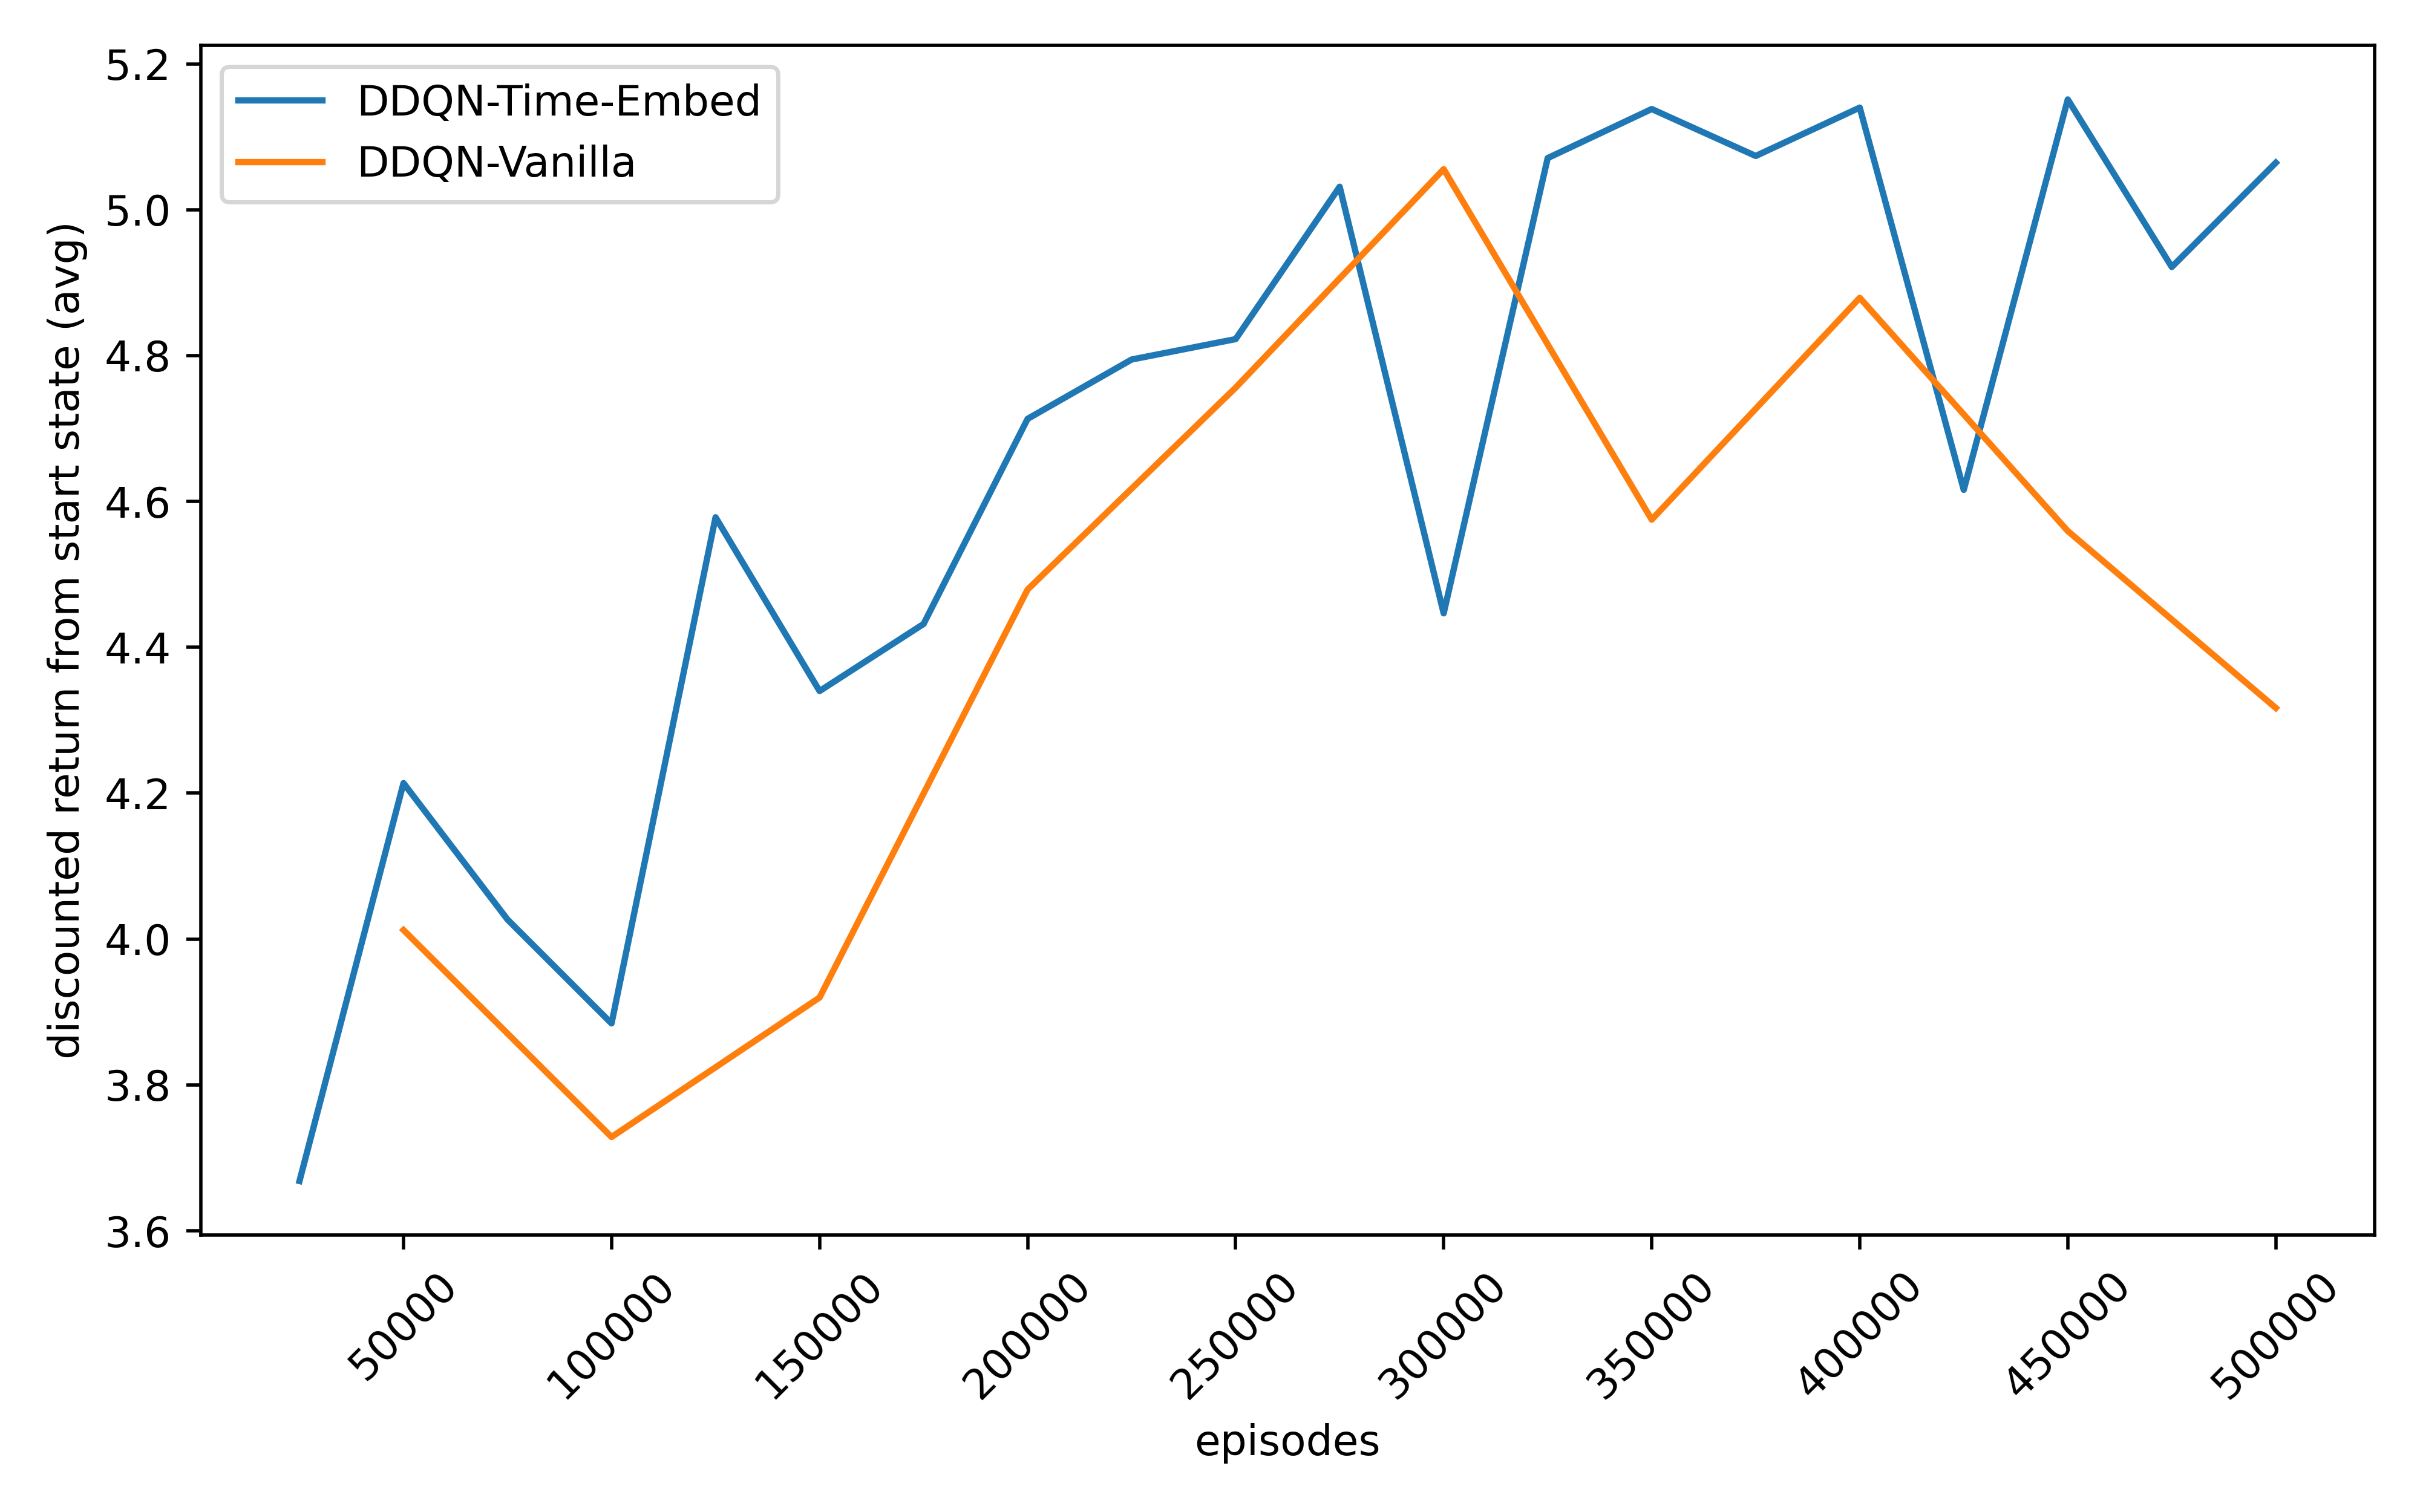
\includegraphics[width=\linewidth]{plots/part3-ddqn-rewards.png}
        \caption{Discounted Return}
    \end{minipage}
    \hfill
    \begin{minipage}{0.32\linewidth}
        \centering
        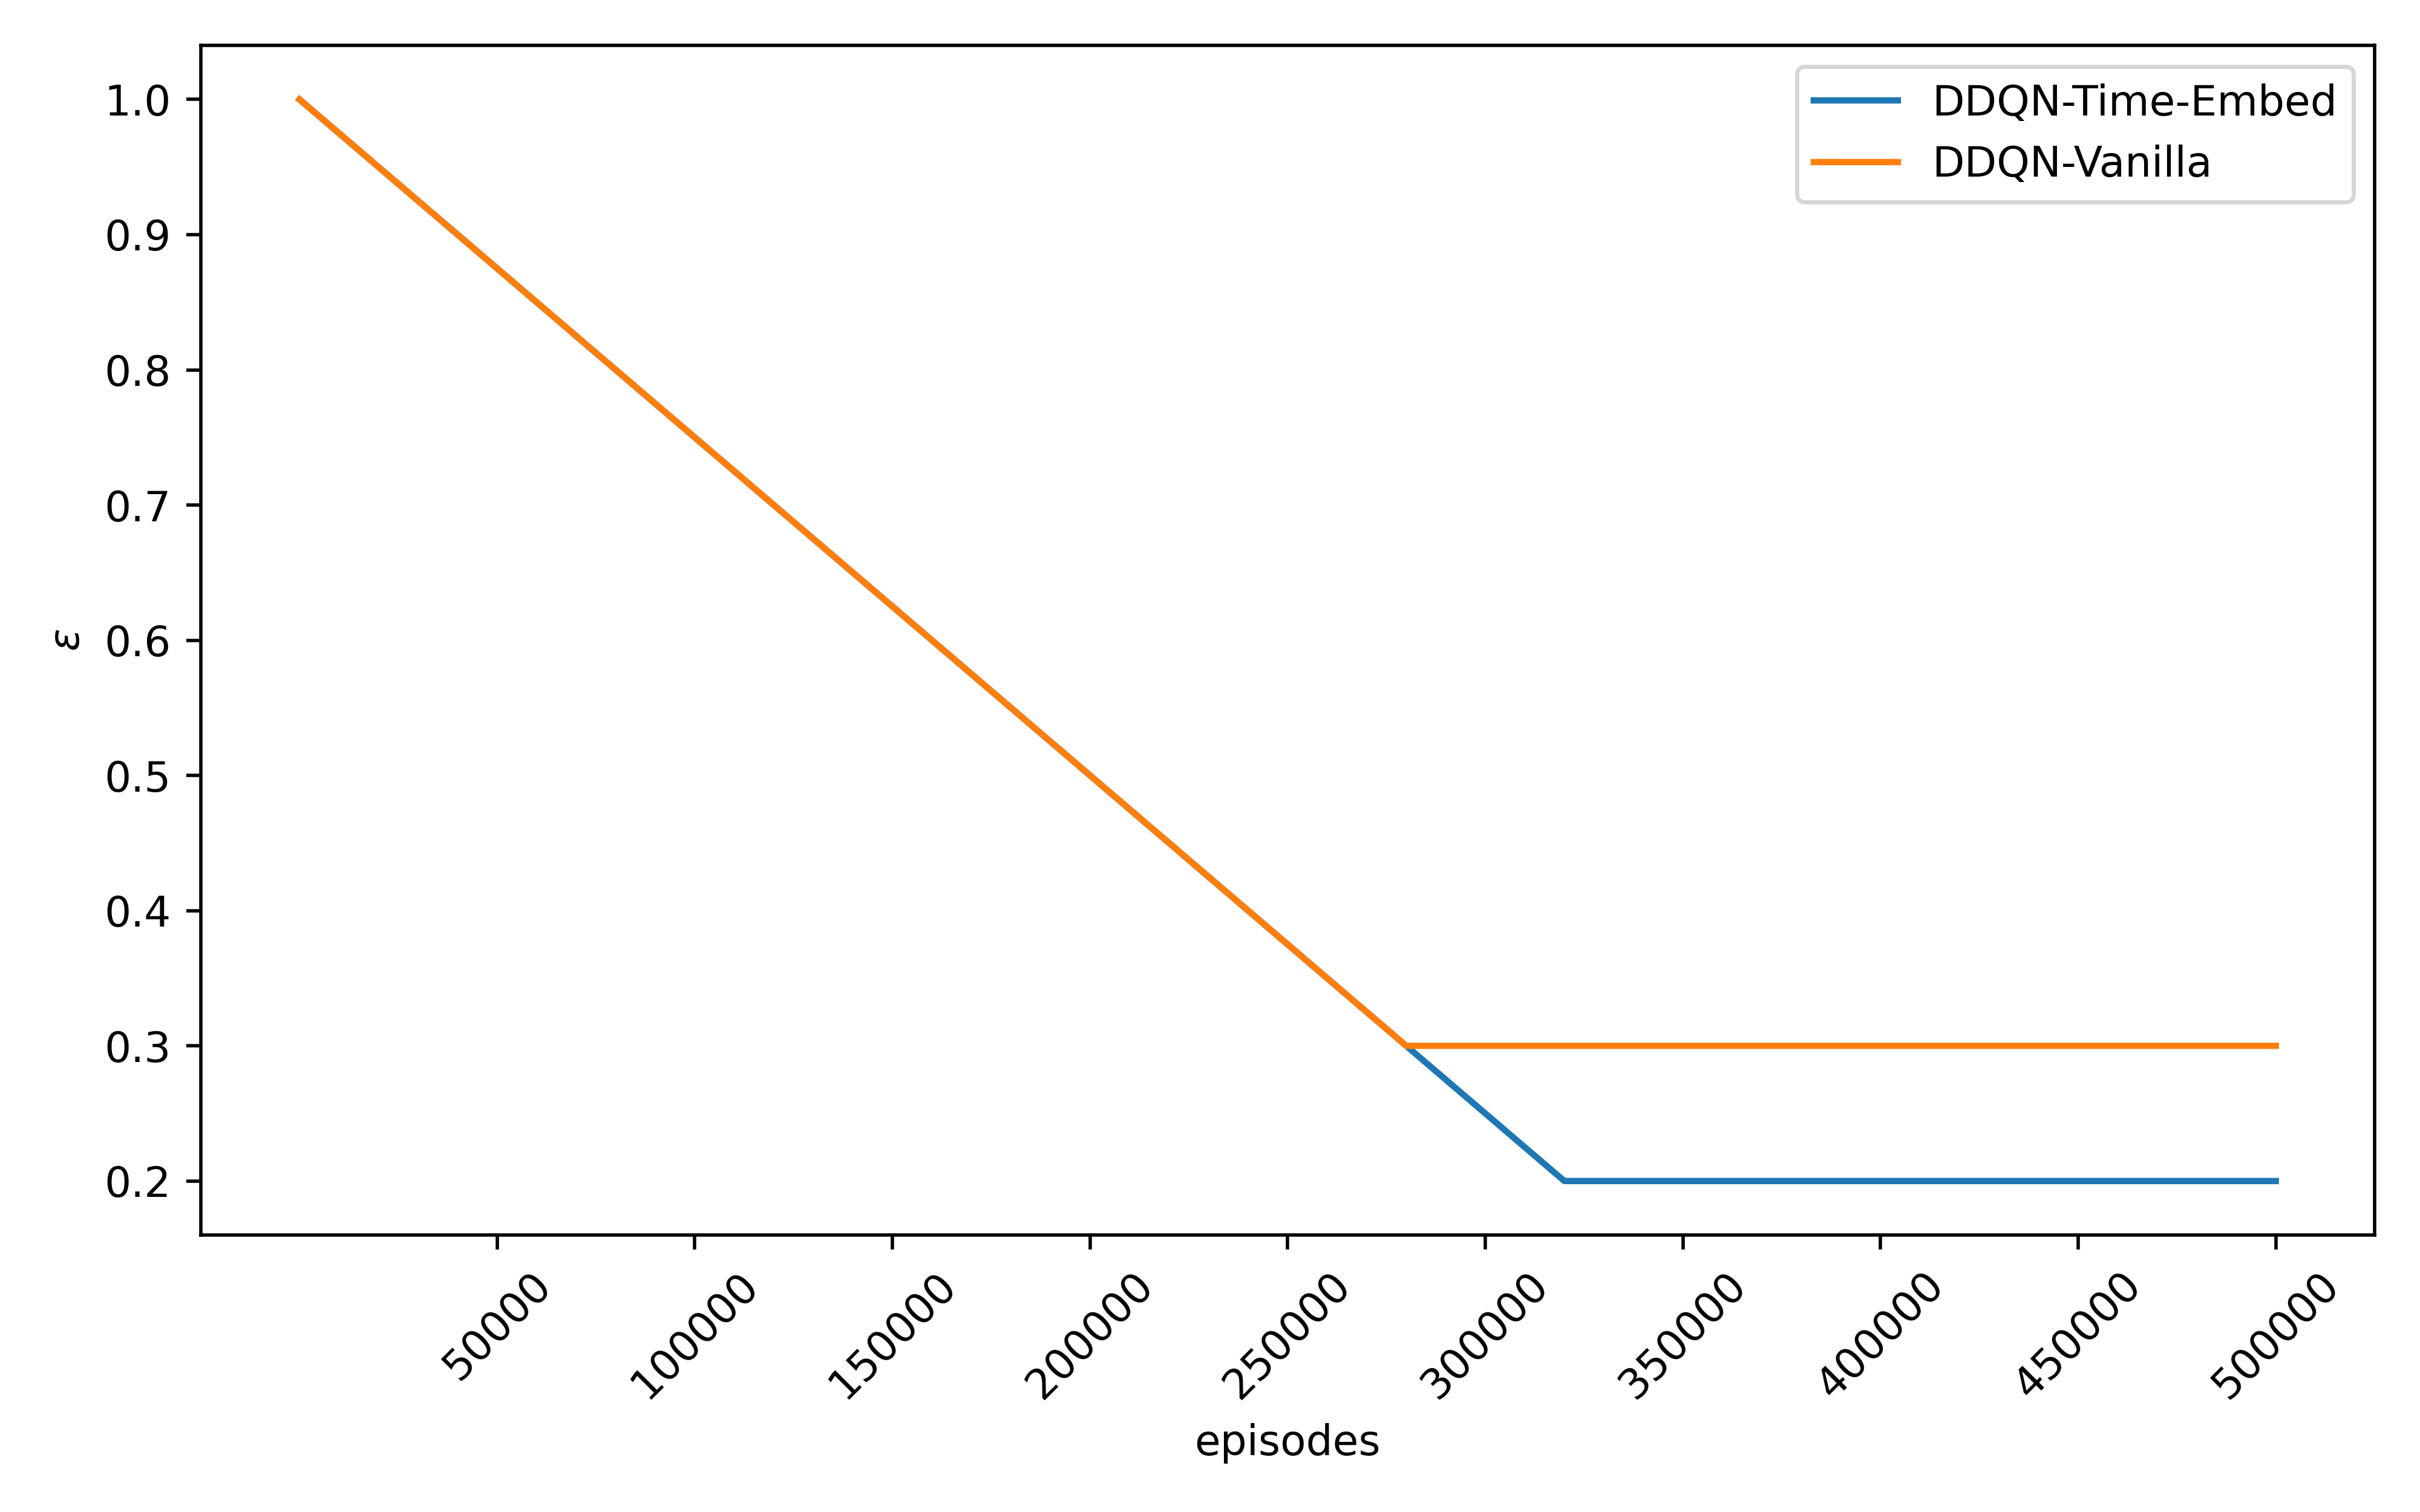
\includegraphics[width=\linewidth]{plots/part3-ddqn-epsilons.png}
        \caption{$\epsilon$ during training}
    \end{minipage}
    \hfill
    \begin{minipage}{0.32\linewidth}
        \centering
        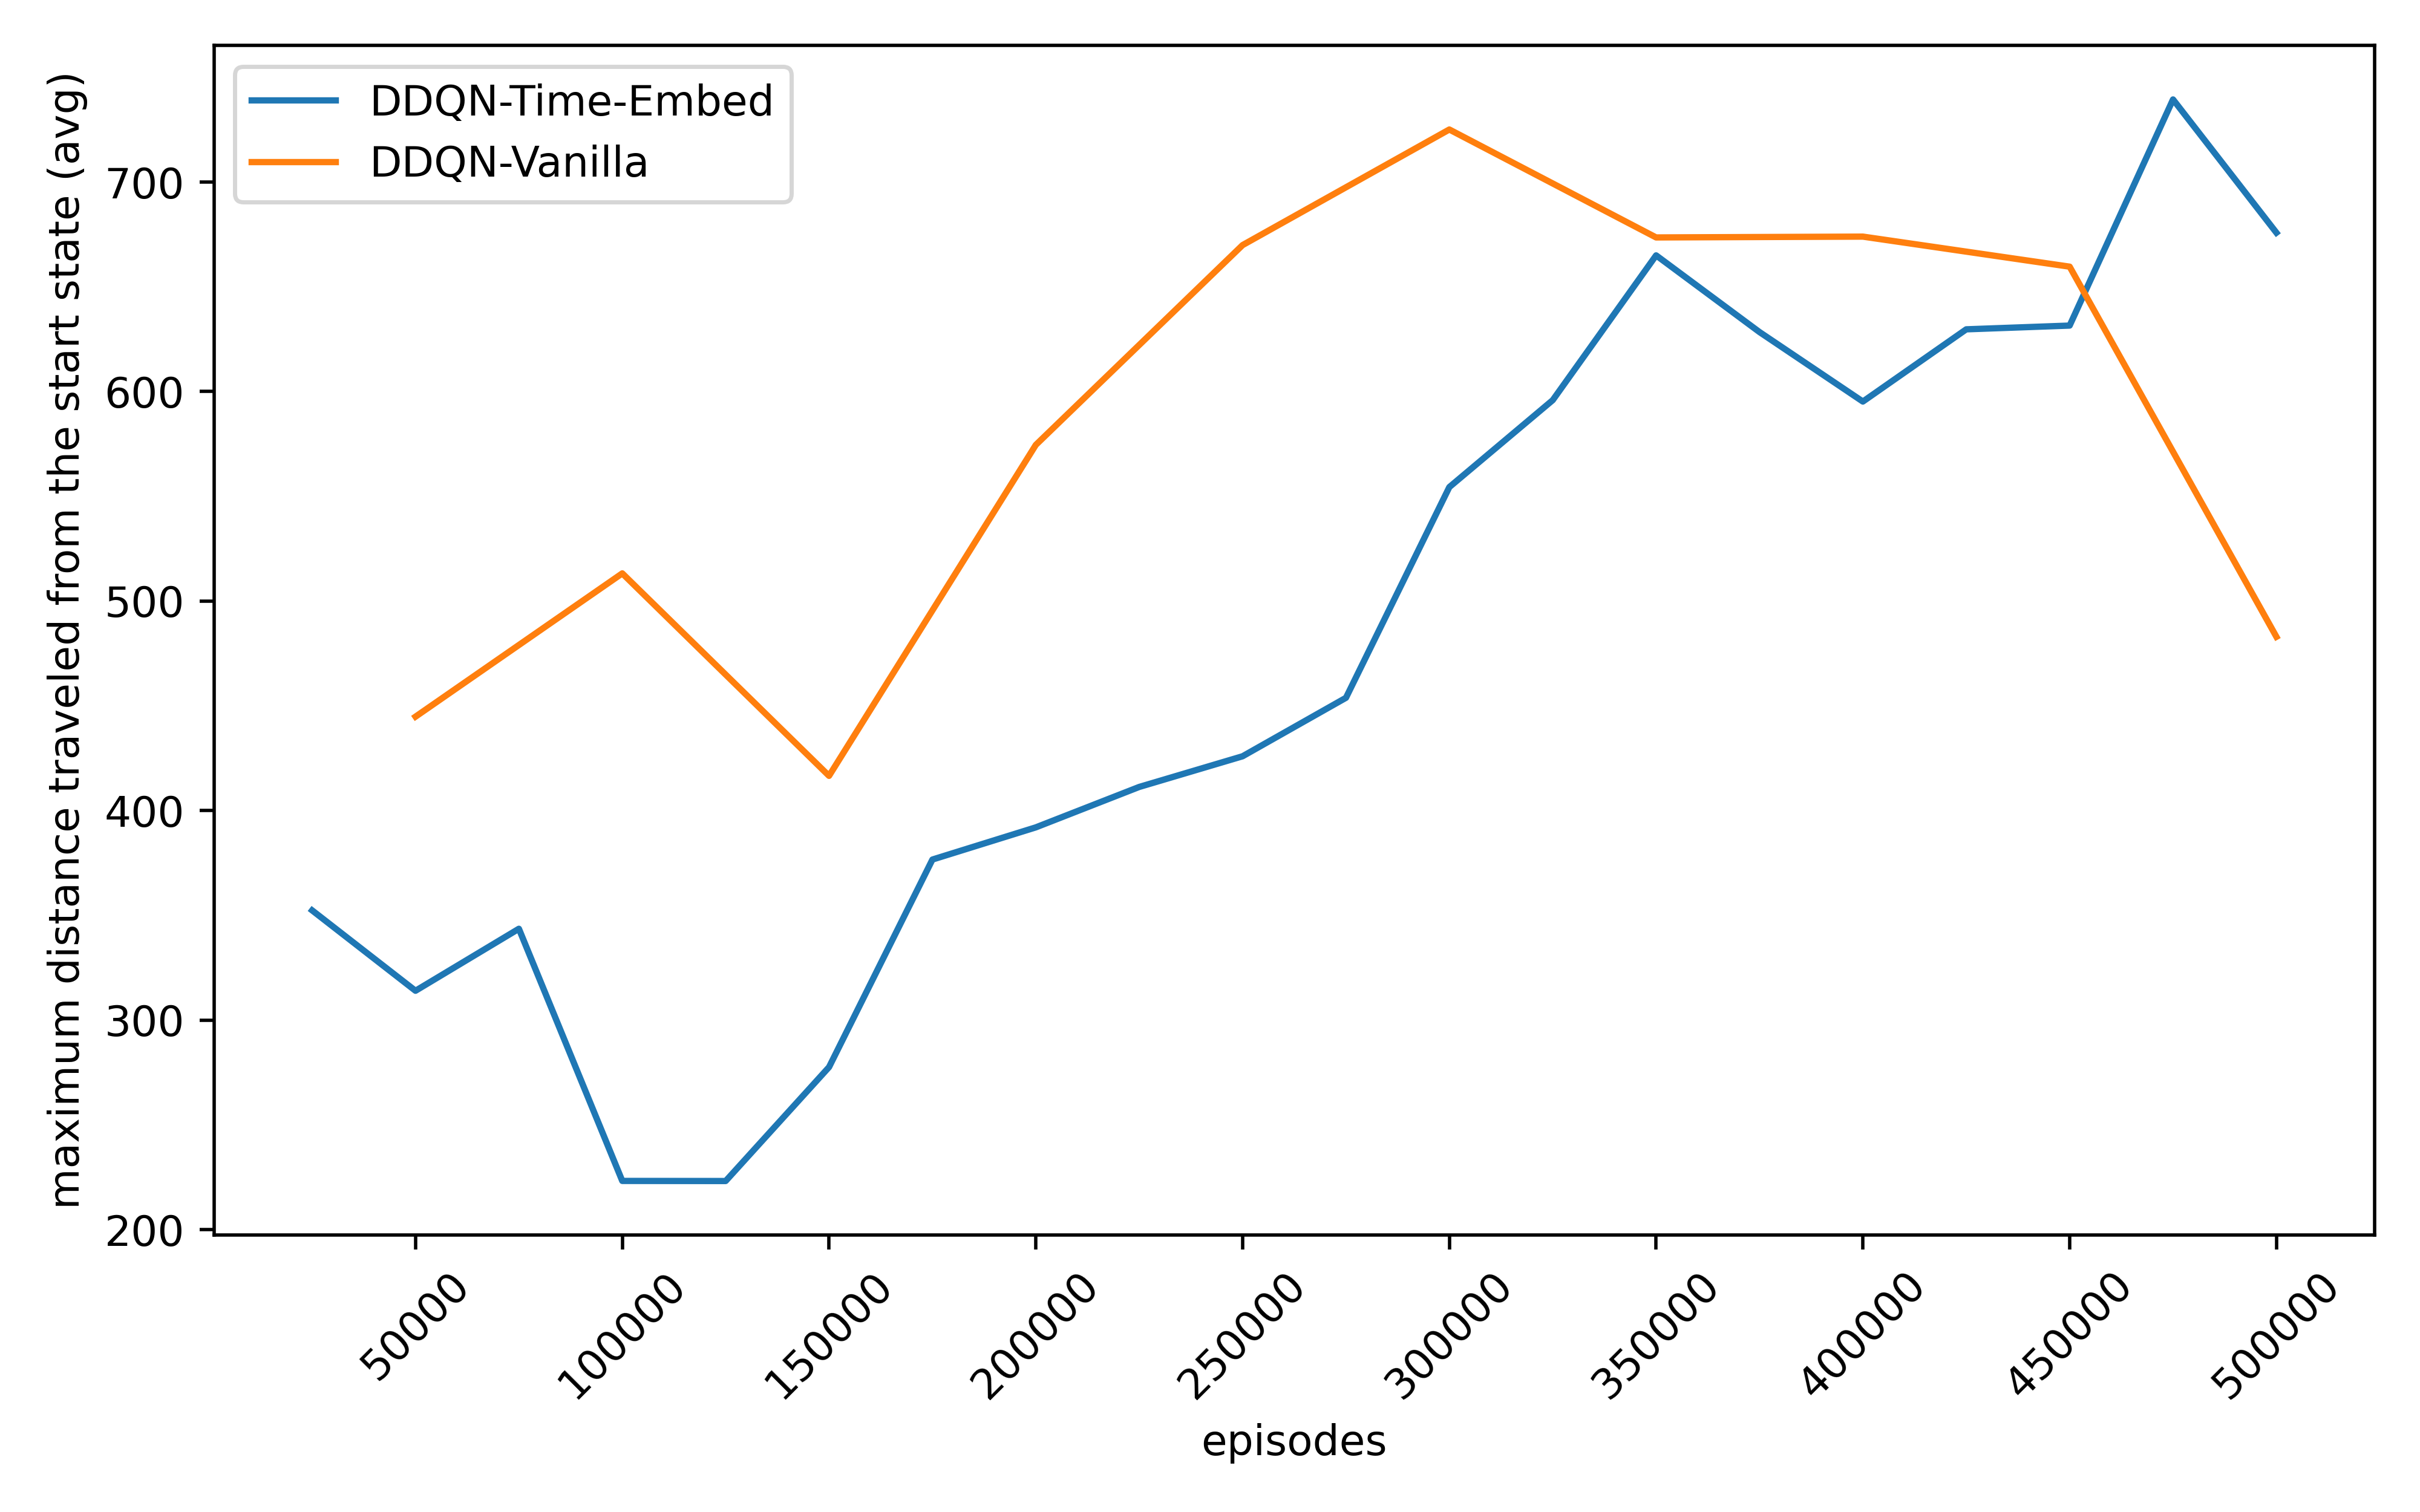
\includegraphics[width=\linewidth]{plots/part3-ddqn-distances.png}
        \caption{Distance Traveled}
    \end{minipage}

    \vspace{0.5em}

    % Second Row - Plots
    \begin{minipage}{0.32\linewidth}
        \centering
        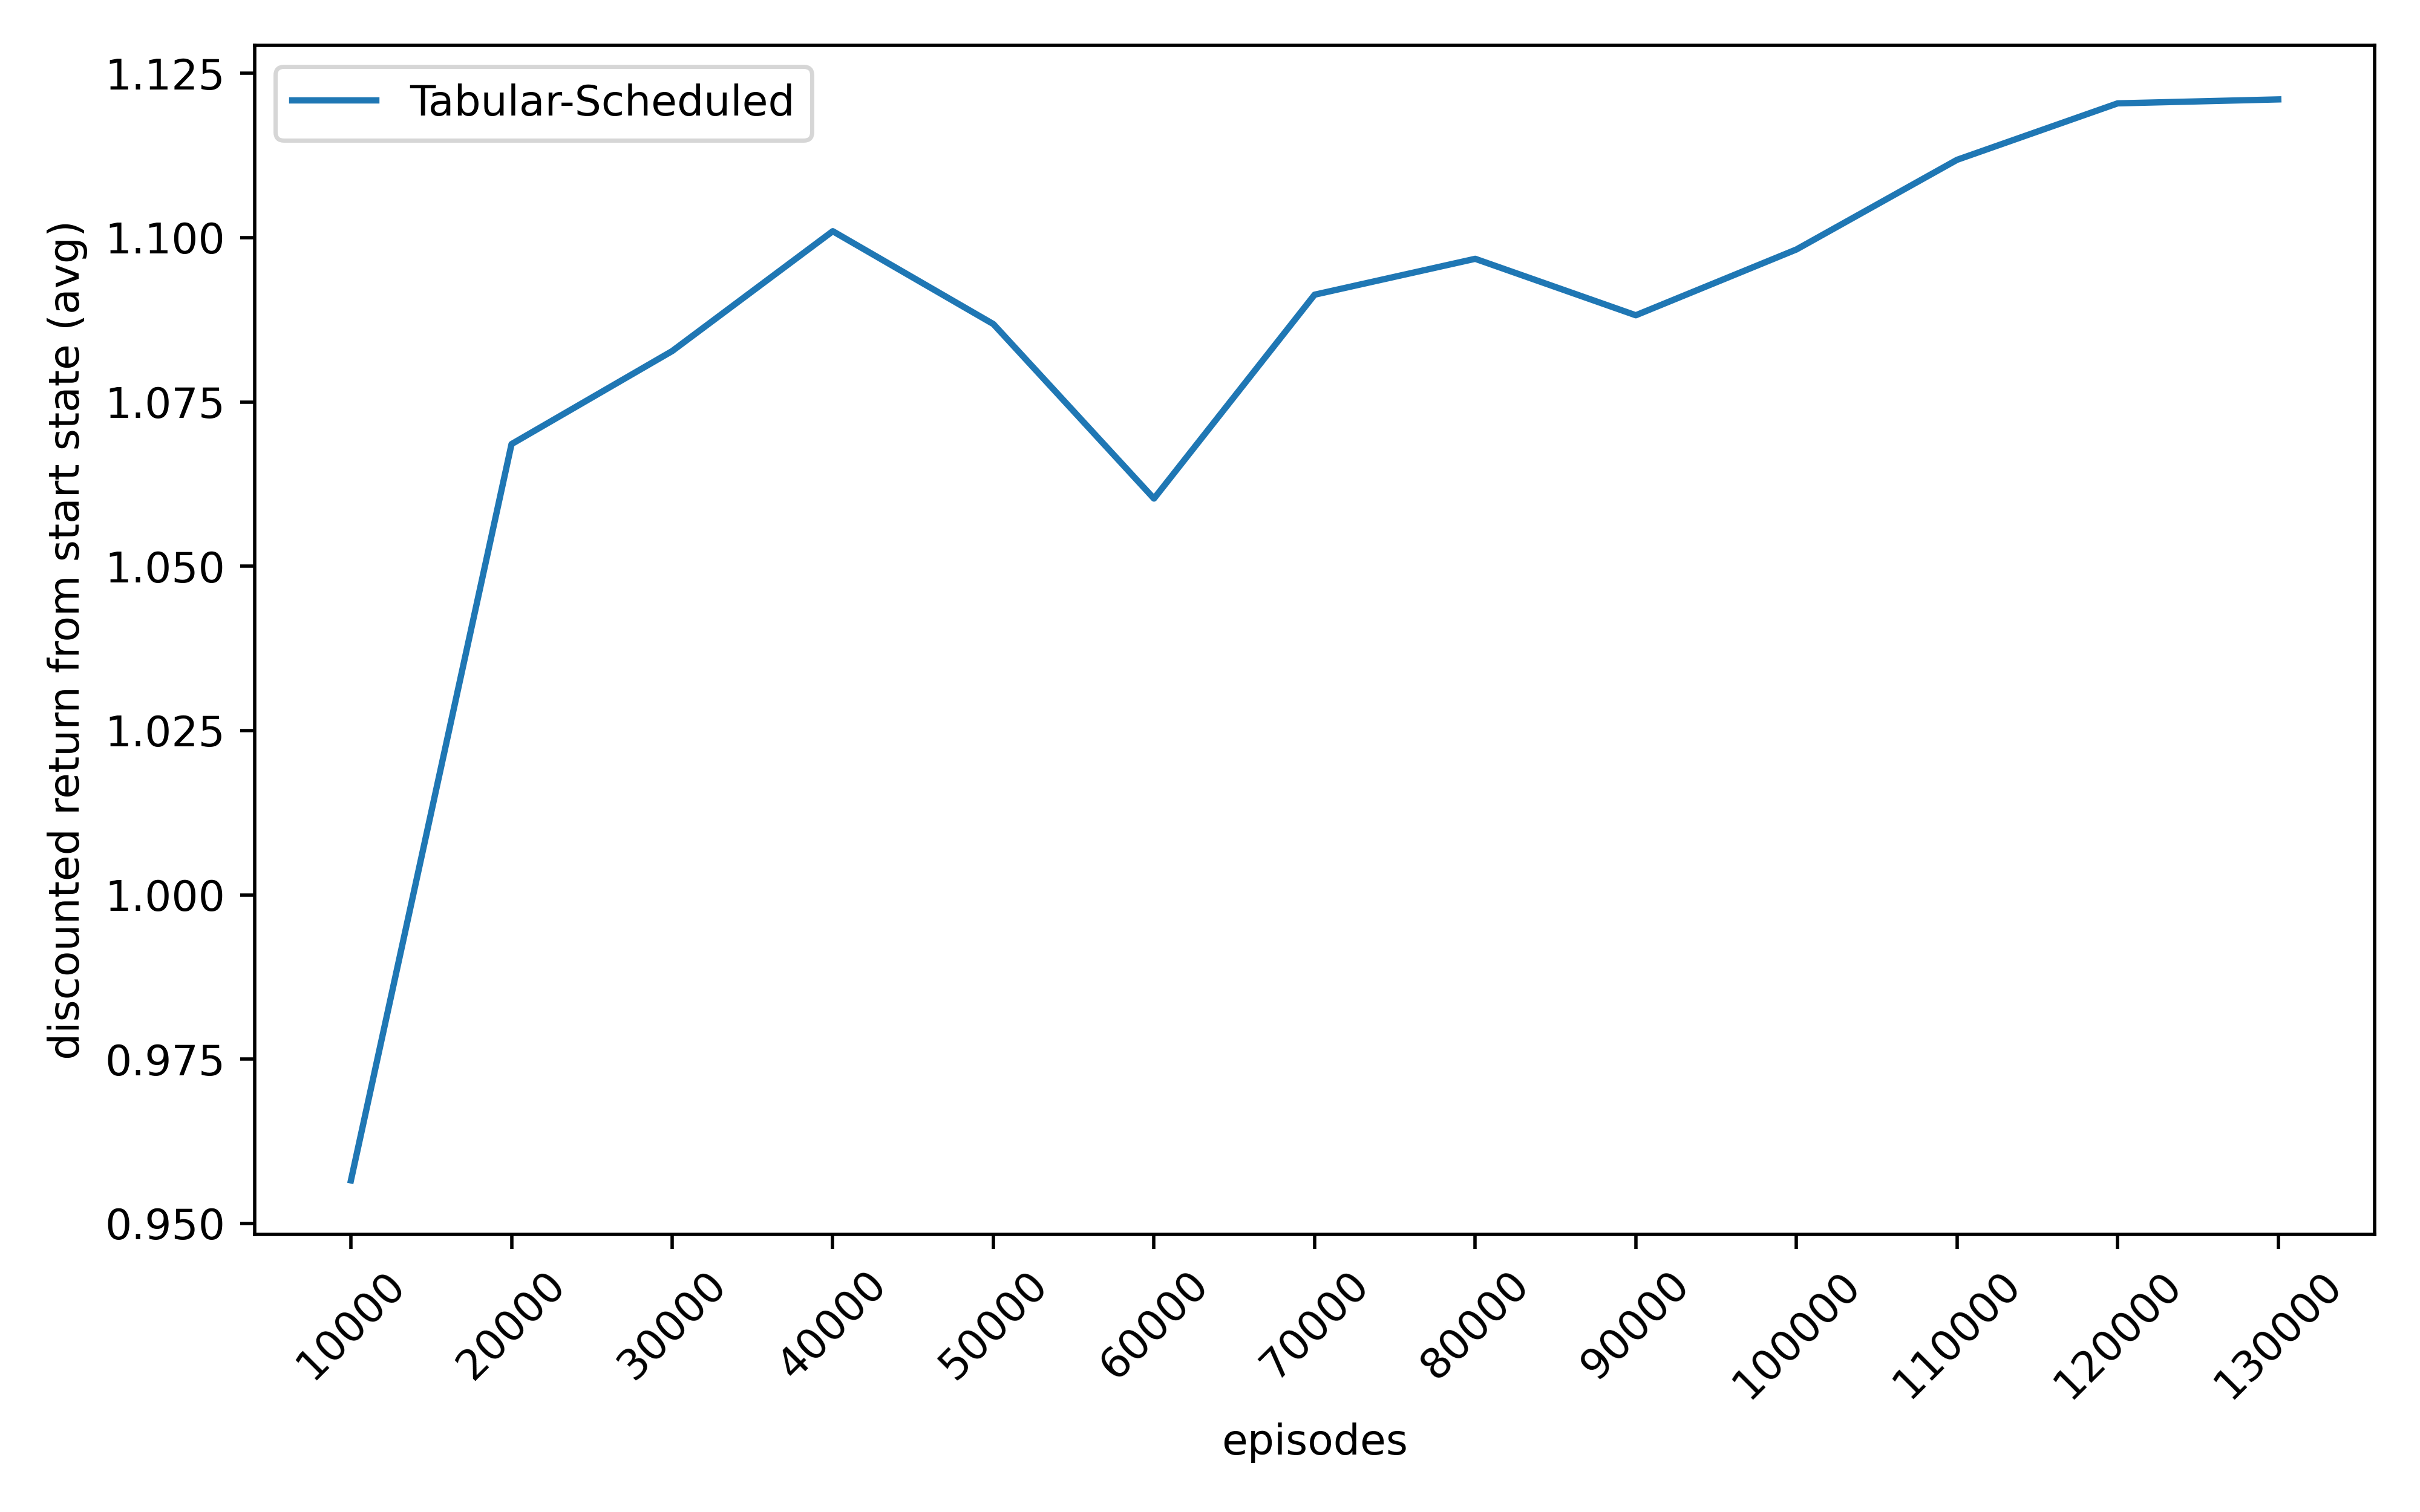
\includegraphics[width=\linewidth]{plots/part3-tabular-rewards.png}
        \caption{Discounted Return}
    \end{minipage}
    \hfill
    \begin{minipage}{0.32\linewidth}
        \centering
        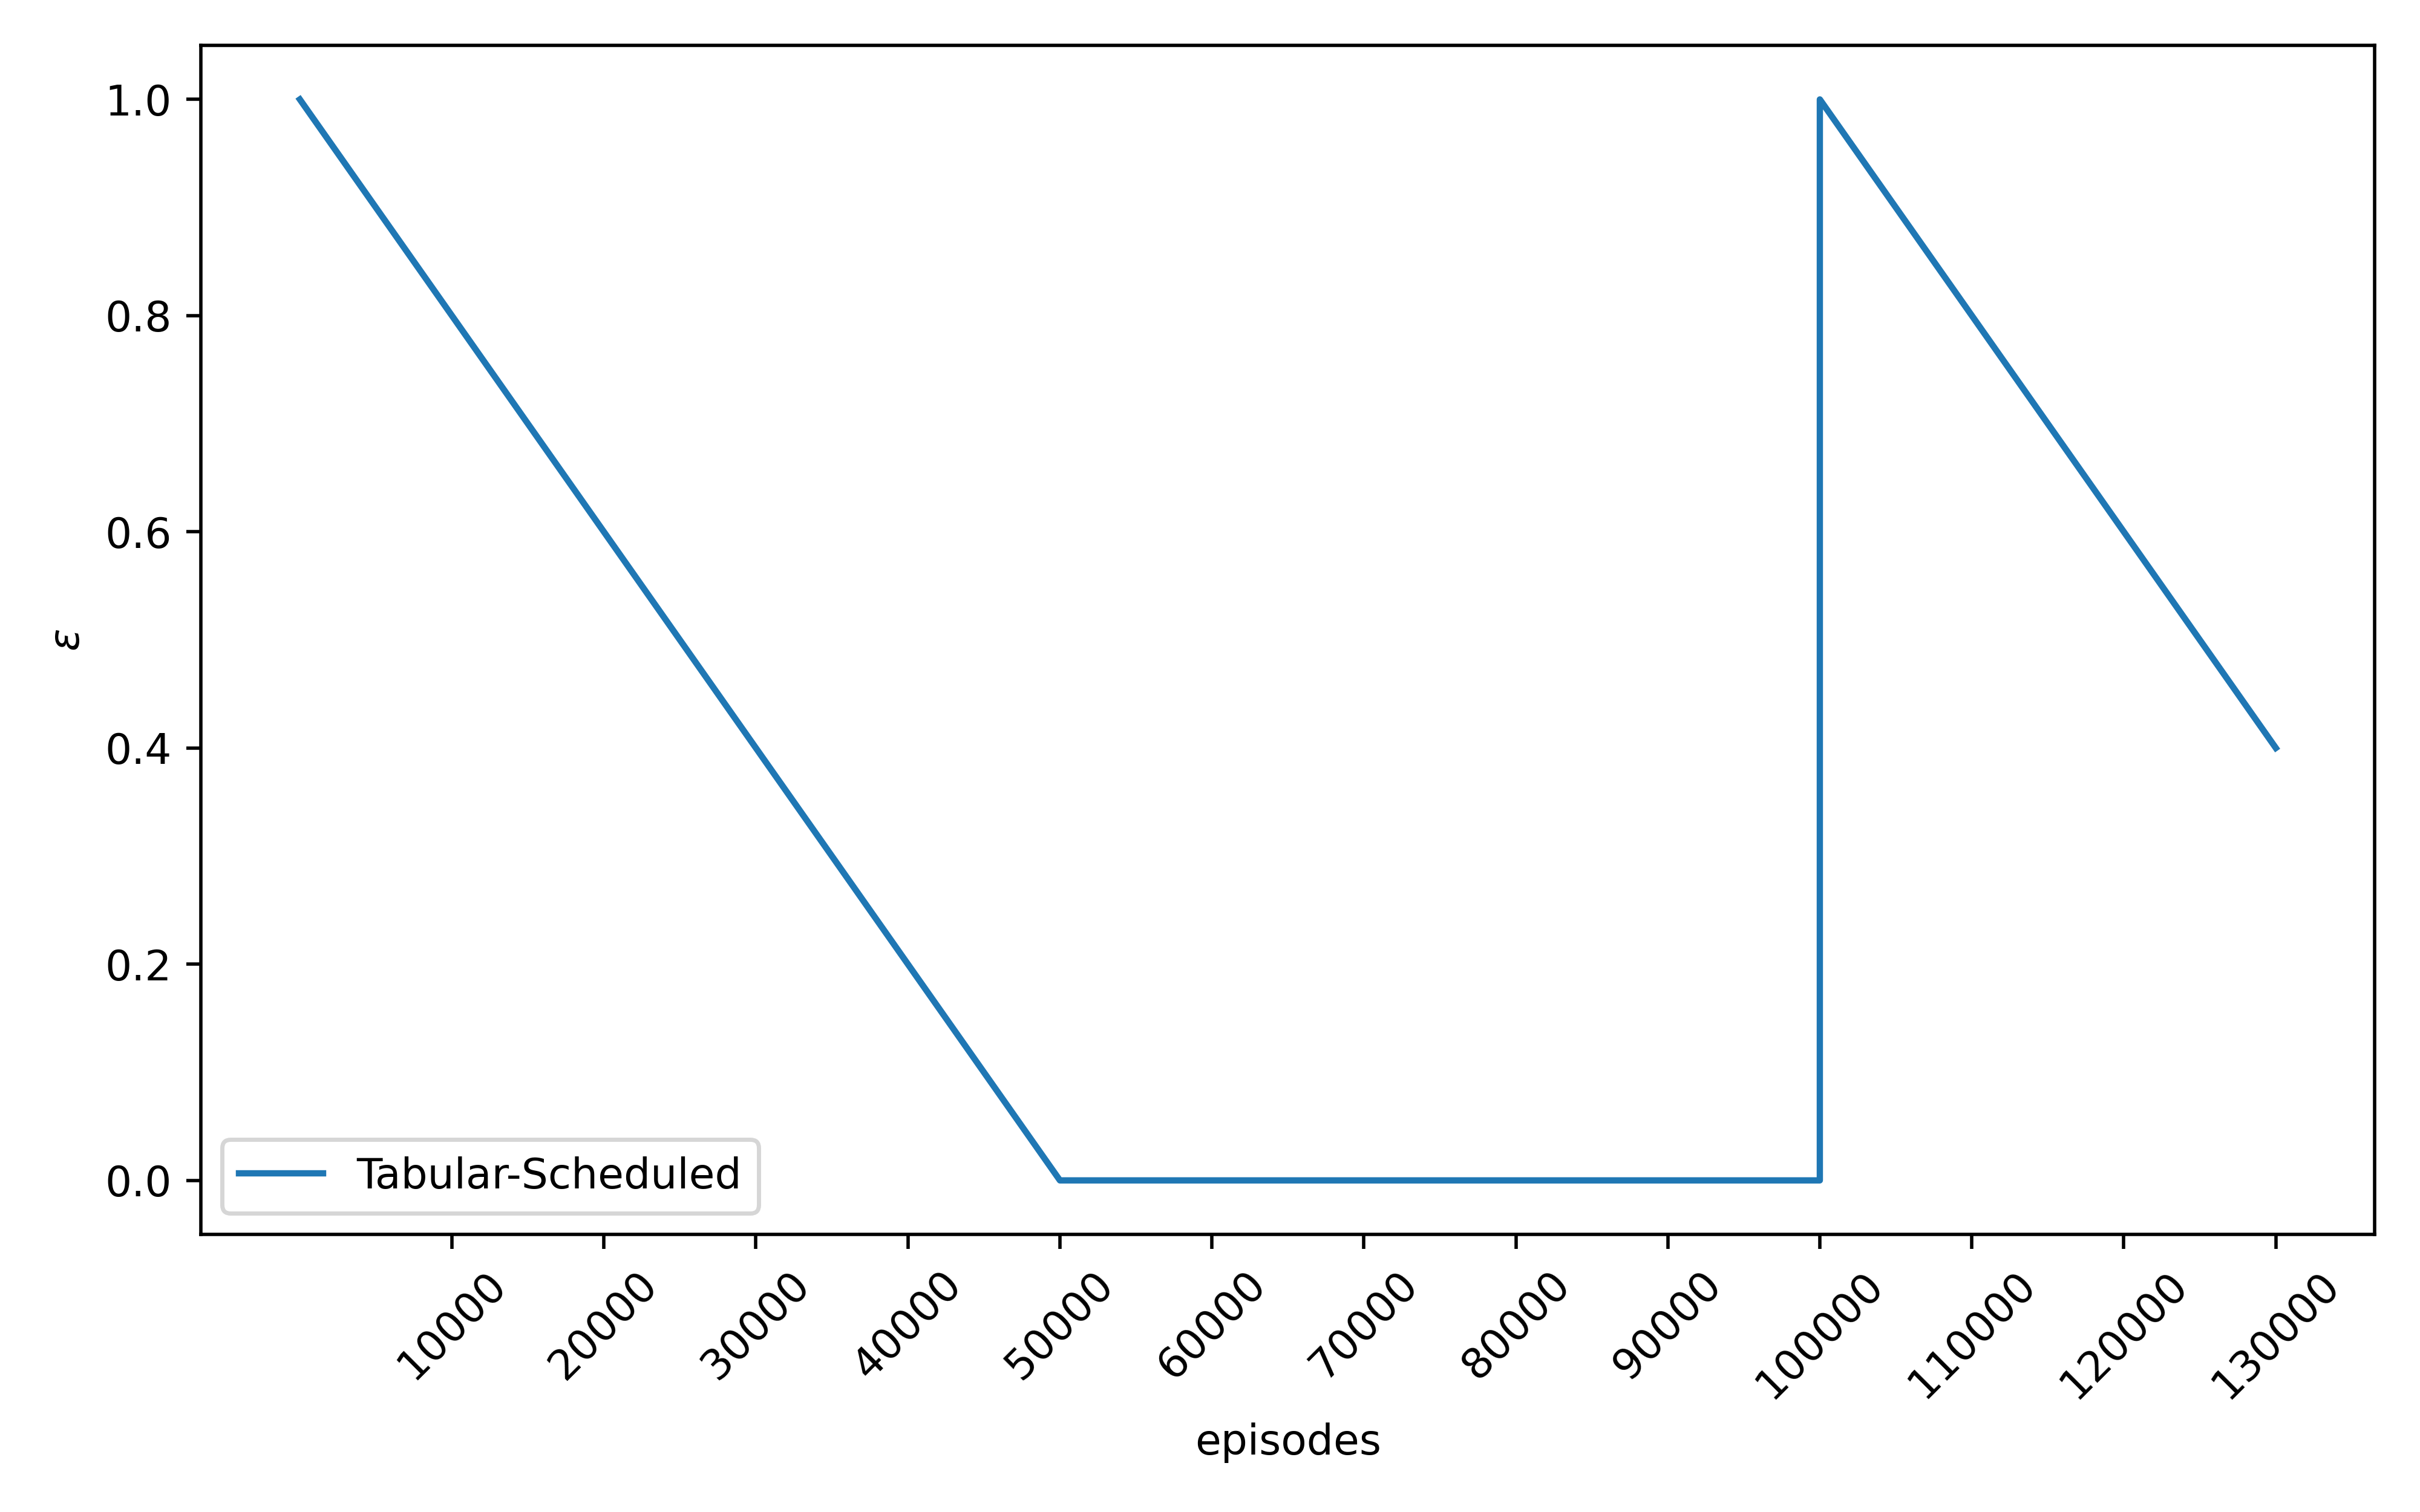
\includegraphics[width=\linewidth]{plots/part3-tabular-epsilons.png}
        \caption{$\epsilon$ during training}

    \end{minipage}
    \hfill
    \begin{minipage}{0.32\linewidth}
        \centering
        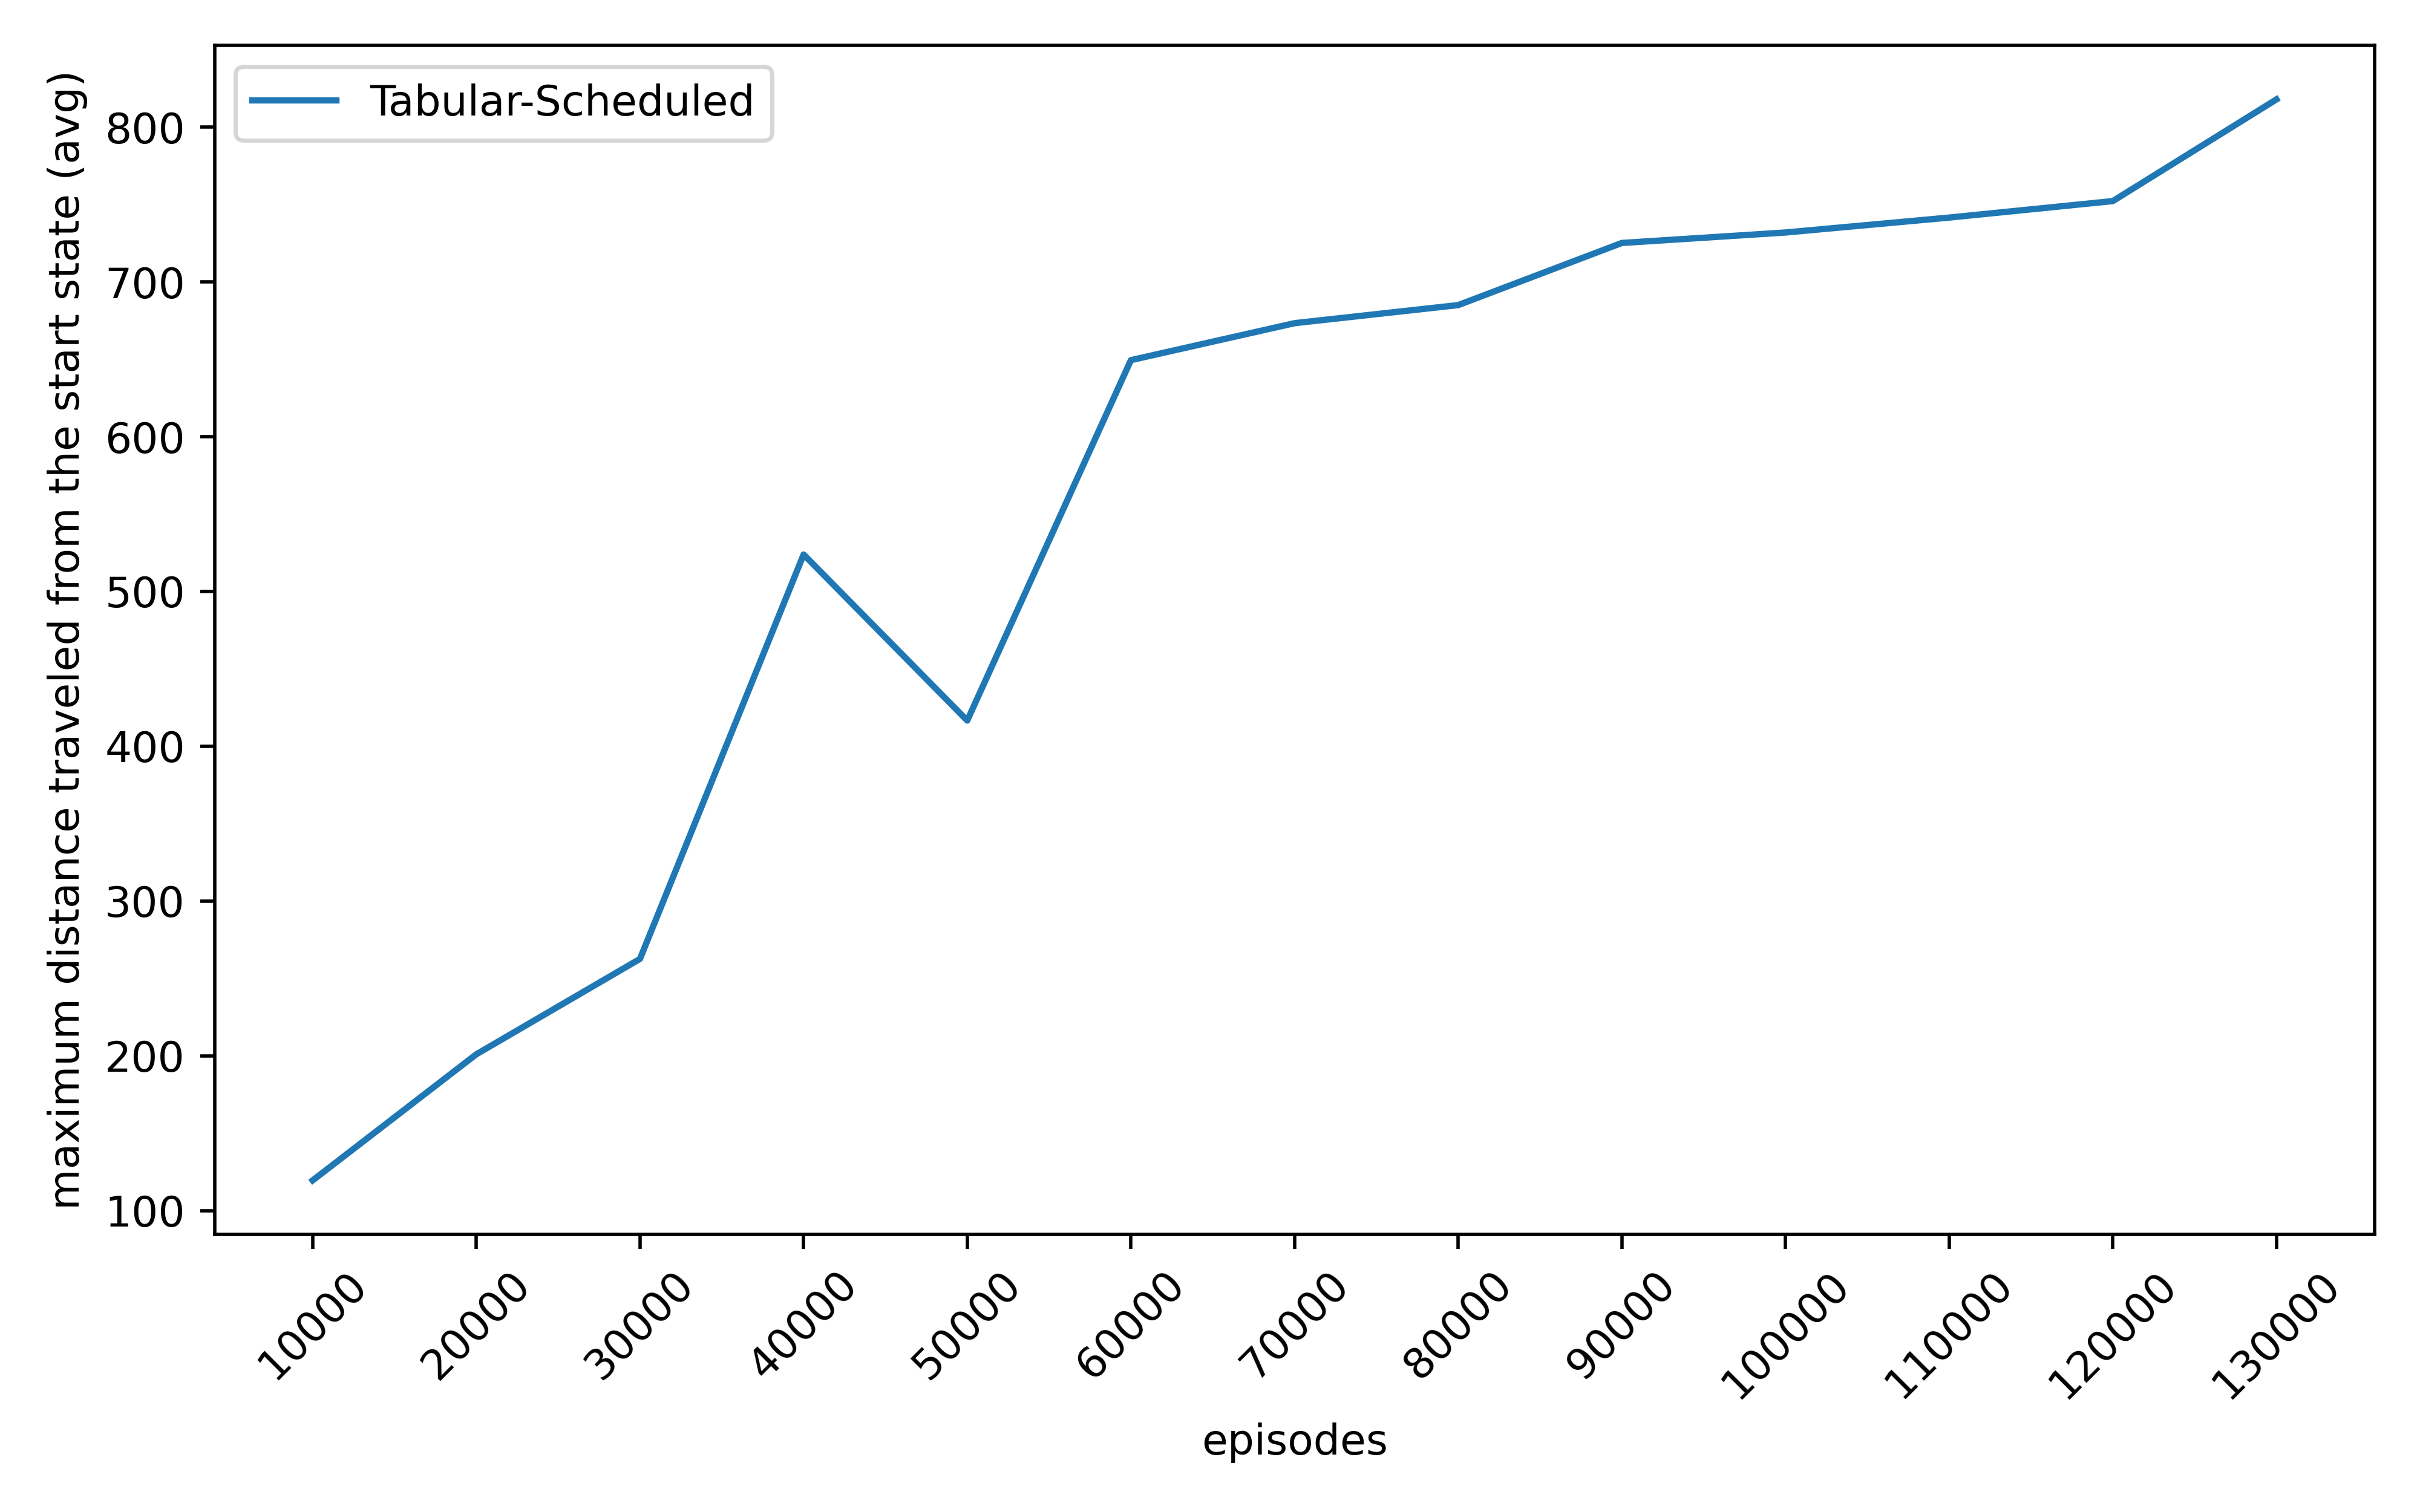
\includegraphics[width=\linewidth]{plots/part3-tabular-distances.png}
        \caption{Distance Traveled}
    \end{minipage}
\end{figure}


\begin{figure}[H]
    \centering

    % Three Tables Side by Side
    \begin{minipage}{0.32\linewidth}
        \centering
        \begin{tabular}{lcc}
            \hline
            Episodes & Discounted & Distance \\
             & Return & Traveled \\
            \hline
            $400,000$ & $5.14$ & $595.23$ \\
            $475,000$ & $4.92$ & $739.43$ \\
            $500,000$ & $5.06$ & $675.82$ \\
            \hline
        \end{tabular}
        \caption{\texttt{DDQN-Time-Embed}}
    \end{minipage}
    \hfill
    \begin{minipage}{0.32\linewidth}
        \centering
        \begin{tabular}{lcc}
            \hline
            Episodes & Discounted & Distance \\
             & Return & Traveled \\
            
            \hline
            $300,000$ & $5.06$ & $725.08$ \\
            $400,000$ & $4.88$ & $673.96$ \\
            $500,000$ & $4.32$ & $482.94$ \\
            \hline
        \end{tabular}
        \caption{\texttt{DDQN-Vanilla}}
    \end{minipage}
    \hfill
    \begin{minipage}{0.32\linewidth}
        \centering
        \begin{tabular}{lcc}
            \hline
            Episodes & Discounted & Distance \\
             & Return & Traveled \\
            \hline
            $50,000$ & $1.09$ & $416.63$ \\
            $100,000$ & $1.10$ & $731.93$ \\
            $130,000$ & $1.12$ & $817.92$ \\
            \hline
        \end{tabular}
        \caption{\texttt{Tabular-Scheduled}}
    \end{minipage}
    \label{fig:part3-time}
\end{figure}

\subsection{Experiments: \texttt{DDQN}}\label{sec:ddqn}
\begin{enumerate}
    \item Both \texttt{DDQN} trained with $\gamma = 0.98, \alpha = 0.1$. \texttt{continuous} observations. The architecture used has the same embedding described in \nameref{sec:arch} but $$64 \texttt{ (input layer)} \to 128 \to 128 \to 64 \to 5 \texttt{ (action layer)}$$ units  respectively in the Neural Network. \texttt{AdamW(lr = 0.0001, amsgrad = True)} is used for training with batch size $512$ and $\tau = 0.005$.

    
    \item \texttt{DDQN-Time-Embed} Reward described in \nameref{sec:reward_design} and $\epsilon$ decreased linearly from $1.0$ to $0.2$ in $320,000$ iterations then kept constant. 
    \item \texttt{DDQN-Vanilla} Reward same as original, \autoref{eqn:reward_vanilla} and $\epsilon$ decreased linearly from $1.0$ to $0.3$ in $280,000$ iterations then kept constant.

    \item Neither of these models would fit in the $2$-hours time limit, and the training time also make it difficult to discover hyper-parameters.
\end{enumerate}
\subsection{\texttt{BestAgent: Tabular-Scheduled}}
\begin{enumerate}
\item We trained the \texttt{Tabular} agent for $100,000$ episodes with $\gamma =  0.90, \alpha = 0.1$ and $\epsilon$ decreased linearly from $1.0$ to $0.0$ in $50,000$ episodes. After $100,000$ episodes we train it with $\gamma = 0.90, \alpha = 0.01$ for $30,000$ episodes. $\epsilon$ follows the same schedule as before.
\item Over $100,000$ seeds from $0$ to $99,999$, the \texttt{Tabular-Scheduled} policy gave an average distance $812.11$ with standard deviation $276.30$. 
\end{enumerate}
\section{Viva Feedback}
\begin{enumerate}
\item 
The \texttt{discrete DQN} implementation is not ideal. The speed levels and distance levels are discretized but have an inherent ordering. Using an embedding layer introduces entanglement into otherwise ordered and separable states, increasing the data requirement for effective learning.

\item This is reflected in the lower performance of \texttt{DQN discrete} and slower initial learning (see \autoref{fig:part2-distance}).

\item A naive strategy is to keep driving at speed~$1$. Other cars have speed~$1$ or~$2$. Over a total of $1000$ episodes, the distance traveled is $0.3 \times 1000 \times 1 = 300$, where $0.3$ is the time per step. The agent does not need to switch any lanes and will not collide.
\end{enumerate}

\end{document}
